% Options for packages loaded elsewhere
\PassOptionsToPackage{unicode}{hyperref}
\PassOptionsToPackage{hyphens}{url}
%
\documentclass[
  12pt,
]{article}
\usepackage{amsmath,amssymb}
\usepackage{iftex}
\ifPDFTeX
  \usepackage[T1]{fontenc}
  \usepackage[utf8]{inputenc}
  \usepackage{textcomp} % provide euro and other symbols
\else % if luatex or xetex
  \usepackage{unicode-math} % this also loads fontspec
  \defaultfontfeatures{Scale=MatchLowercase}
  \defaultfontfeatures[\rmfamily]{Ligatures=TeX,Scale=1}
\fi
\usepackage{lmodern}
\ifPDFTeX\else
  % xetex/luatex font selection
\fi
% Use upquote if available, for straight quotes in verbatim environments
\IfFileExists{upquote.sty}{\usepackage{upquote}}{}
\IfFileExists{microtype.sty}{% use microtype if available
  \usepackage[]{microtype}
  \UseMicrotypeSet[protrusion]{basicmath} % disable protrusion for tt fonts
}{}
\usepackage{xcolor}
\usepackage[margin=1in]{geometry}
\usepackage{color}
\usepackage{fancyvrb}
\newcommand{\VerbBar}{|}
\newcommand{\VERB}{\Verb[commandchars=\\\{\}]}
\DefineVerbatimEnvironment{Highlighting}{Verbatim}{commandchars=\\\{\}}
% Add ',fontsize=\small' for more characters per line
\usepackage{framed}
\definecolor{shadecolor}{RGB}{248,248,248}
\newenvironment{Shaded}{\begin{snugshade}}{\end{snugshade}}
\newcommand{\AlertTok}[1]{\textcolor[rgb]{0.94,0.16,0.16}{#1}}
\newcommand{\AnnotationTok}[1]{\textcolor[rgb]{0.56,0.35,0.01}{\textbf{\textit{#1}}}}
\newcommand{\AttributeTok}[1]{\textcolor[rgb]{0.13,0.29,0.53}{#1}}
\newcommand{\BaseNTok}[1]{\textcolor[rgb]{0.00,0.00,0.81}{#1}}
\newcommand{\BuiltInTok}[1]{#1}
\newcommand{\CharTok}[1]{\textcolor[rgb]{0.31,0.60,0.02}{#1}}
\newcommand{\CommentTok}[1]{\textcolor[rgb]{0.56,0.35,0.01}{\textit{#1}}}
\newcommand{\CommentVarTok}[1]{\textcolor[rgb]{0.56,0.35,0.01}{\textbf{\textit{#1}}}}
\newcommand{\ConstantTok}[1]{\textcolor[rgb]{0.56,0.35,0.01}{#1}}
\newcommand{\ControlFlowTok}[1]{\textcolor[rgb]{0.13,0.29,0.53}{\textbf{#1}}}
\newcommand{\DataTypeTok}[1]{\textcolor[rgb]{0.13,0.29,0.53}{#1}}
\newcommand{\DecValTok}[1]{\textcolor[rgb]{0.00,0.00,0.81}{#1}}
\newcommand{\DocumentationTok}[1]{\textcolor[rgb]{0.56,0.35,0.01}{\textbf{\textit{#1}}}}
\newcommand{\ErrorTok}[1]{\textcolor[rgb]{0.64,0.00,0.00}{\textbf{#1}}}
\newcommand{\ExtensionTok}[1]{#1}
\newcommand{\FloatTok}[1]{\textcolor[rgb]{0.00,0.00,0.81}{#1}}
\newcommand{\FunctionTok}[1]{\textcolor[rgb]{0.13,0.29,0.53}{\textbf{#1}}}
\newcommand{\ImportTok}[1]{#1}
\newcommand{\InformationTok}[1]{\textcolor[rgb]{0.56,0.35,0.01}{\textbf{\textit{#1}}}}
\newcommand{\KeywordTok}[1]{\textcolor[rgb]{0.13,0.29,0.53}{\textbf{#1}}}
\newcommand{\NormalTok}[1]{#1}
\newcommand{\OperatorTok}[1]{\textcolor[rgb]{0.81,0.36,0.00}{\textbf{#1}}}
\newcommand{\OtherTok}[1]{\textcolor[rgb]{0.56,0.35,0.01}{#1}}
\newcommand{\PreprocessorTok}[1]{\textcolor[rgb]{0.56,0.35,0.01}{\textit{#1}}}
\newcommand{\RegionMarkerTok}[1]{#1}
\newcommand{\SpecialCharTok}[1]{\textcolor[rgb]{0.81,0.36,0.00}{\textbf{#1}}}
\newcommand{\SpecialStringTok}[1]{\textcolor[rgb]{0.31,0.60,0.02}{#1}}
\newcommand{\StringTok}[1]{\textcolor[rgb]{0.31,0.60,0.02}{#1}}
\newcommand{\VariableTok}[1]{\textcolor[rgb]{0.00,0.00,0.00}{#1}}
\newcommand{\VerbatimStringTok}[1]{\textcolor[rgb]{0.31,0.60,0.02}{#1}}
\newcommand{\WarningTok}[1]{\textcolor[rgb]{0.56,0.35,0.01}{\textbf{\textit{#1}}}}
\usepackage{longtable,booktabs,array}
\usepackage{calc} % for calculating minipage widths
% Correct order of tables after \paragraph or \subparagraph
\usepackage{etoolbox}
\makeatletter
\patchcmd\longtable{\par}{\if@noskipsec\mbox{}\fi\par}{}{}
\makeatother
% Allow footnotes in longtable head/foot
\IfFileExists{footnotehyper.sty}{\usepackage{footnotehyper}}{\usepackage{footnote}}
\makesavenoteenv{longtable}
\usepackage{graphicx}
\makeatletter
\def\maxwidth{\ifdim\Gin@nat@width>\linewidth\linewidth\else\Gin@nat@width\fi}
\def\maxheight{\ifdim\Gin@nat@height>\textheight\textheight\else\Gin@nat@height\fi}
\makeatother
% Scale images if necessary, so that they will not overflow the page
% margins by default, and it is still possible to overwrite the defaults
% using explicit options in \includegraphics[width, height, ...]{}
\setkeys{Gin}{width=\maxwidth,height=\maxheight,keepaspectratio}
% Set default figure placement to htbp
\makeatletter
\def\fps@figure{htbp}
\makeatother
\setlength{\emergencystretch}{3em} % prevent overfull lines
\providecommand{\tightlist}{%
  \setlength{\itemsep}{0pt}\setlength{\parskip}{0pt}}
\setcounter{secnumdepth}{-\maxdimen} % remove section numbering
% definitions for citeproc citations
\NewDocumentCommand\citeproctext{}{}
\NewDocumentCommand\citeproc{mm}{%
  \begingroup\def\citeproctext{#2}\cite{#1}\endgroup}
\makeatletter
 % allow citations to break across lines
 \let\@cite@ofmt\@firstofone
 % avoid brackets around text for \cite:
 \def\@biblabel#1{}
 \def\@cite#1#2{{#1\if@tempswa , #2\fi}}
\makeatother
\newlength{\cslhangindent}
\setlength{\cslhangindent}{1.5em}
\newlength{\csllabelwidth}
\setlength{\csllabelwidth}{3em}
\newenvironment{CSLReferences}[2] % #1 hanging-indent, #2 entry-spacing
 {\begin{list}{}{%
  \setlength{\itemindent}{0pt}
  \setlength{\leftmargin}{0pt}
  \setlength{\parsep}{0pt}
  % turn on hanging indent if param 1 is 1
  \ifodd #1
   \setlength{\leftmargin}{\cslhangindent}
   \setlength{\itemindent}{-1\cslhangindent}
  \fi
  % set entry spacing
  \setlength{\itemsep}{#2\baselineskip}}}
 {\end{list}}
\usepackage{calc}
\newcommand{\CSLBlock}[1]{\hfill\break\parbox[t]{\linewidth}{\strut\ignorespaces#1\strut}}
\newcommand{\CSLLeftMargin}[1]{\parbox[t]{\csllabelwidth}{\strut#1\strut}}
\newcommand{\CSLRightInline}[1]{\parbox[t]{\linewidth - \csllabelwidth}{\strut#1\strut}}
\newcommand{\CSLIndent}[1]{\hspace{\cslhangindent}#1}
\usepackage{titling}
\usepackage{savesym}
\usepackage{amsmath}
\savesymbol{arrowvert}
\usepackage{amsthm}
\usepackage{newtx}
\restoresymbol{NTX}{arrowvert}
\usepackage{rotating}
\usepackage{setspace}
\usepackage{indentfirst}
\usepackage{changepage}
\doublespacing
\pretitle{\begin{center}\fontsize{12pt}{14pt}\selectfont\rmfamily\bfseries}
\posttitle{\par\end{center}\vspace{2cm}}
\preauthor{\begin{center}\fontsize{12pt}{14pt}\selectfont\rmfamily}
\postauthor{\par\end{center}}
\predate{\begin{center}\fontsize{12pt}{14pt}\selectfont\rmfamily}
\postdate{\par\end{center}\vspace{5cm}}
\pagenumbering{gobble}
\usepackage{float}
\usepackage{wrapfig}
\usepackage{sectsty}
\sectionfont{\normalsize}
\subsectionfont{\normalsize}
\subsubsectionfont{\normalsize}
\usepackage{booktabs}
\usepackage{longtable}
\usepackage{array}
\usepackage{multirow}
\usepackage{wrapfig}
\usepackage{float}
\usepackage{colortbl}
\usepackage{pdflscape}
\usepackage{tabu}
\usepackage{threeparttable}
\usepackage{threeparttablex}
\usepackage[normalem]{ulem}
\usepackage{makecell}
\usepackage{xcolor}
\ifLuaTeX
  \usepackage{selnolig}  % disable illegal ligatures
\fi
\usepackage{bookmark}
\IfFileExists{xurl.sty}{\usepackage{xurl}}{} % add URL line breaks if available
\urlstyle{same}
\hypersetup{
  pdftitle={Modeling the Effect of the RapidRide Program on Bus Reliability in Seattle, WA, Using Regression and Bayesian Additive Regression Trees},
  pdfauthor={Peter Silverstein},
  hidelinks,
  pdfcreator={LaTeX via pandoc}}

\title{Modeling the Effect of the RapidRide Program on Bus Reliability
in Seattle, WA, Using Regression and Bayesian Additive Regression Trees}
\author{Peter Silverstein}
\date{}

\begin{document}
\maketitle

\begin{adjustwidth}{1.5in}{1.5in}
\begin{center}
    \fontsize{12pt}{14pt}\selectfont
    {Submitted in partial fulfillment of the requirements for the degree of Master of   Arts under the Executive Committee of the Graduate School of Arts and Sciences}\\[1cm]
    {COLUMBIA UNIVERSITY}\\[1cm]
    {Advisor: Dr. Edwin Grimsley}\\[0.5cm]
    {2025}
\end{center}
\end{adjustwidth}

\newpage

\vspace*{\fill}
\begin{center}
    \fontsize{12pt}{14pt}\selectfont
    {© 2025}\\[0.5cm]
    {Peter Silverstein}\\[0.5cm]
    {All Rights Reserved}\\
\end{center}
\newpage

\tableofcontents

\newpage
\pagenumbering{arabic}

\section{0. Abstract}\label{abstract}

Mass transit systems are a crucial piece in the fabric of any urban
environment. They allow people who do not own cars to access the far
reaches of a city and provide a more sustainable alternative to single
occupancy vehicle traffic. In large part, the success of a transit system
is dependent on its ability to get people where they want to go and do
so with reliability. The present research examines a transit
intervention, the RapidRide bus route upgrade program in Seattle,
Washington, and seeks to determine whether it has a positive effect on
bus reliability. Linear regression models and a Bayesian Additive
Regression Trees model are applied in a causal inference setting to
estimate the average treatment effect of the RapidRide treatment on the
bus routes that have been upgraded. All models find that the RapidRide
treatment improves reliability. Median estimates for this treatment
effect vary by model, and range from a 15 second improvement to a nearly
60 second improvement as a result of the intervention. Further,
different models provide different uncertainty associated with this
effect, indicating that the variability of the treatment effect is also
an interesting point of study. Because reliability is an attribute that
is highly valued by mass transit riders and because better reliability
is associated with a greater ability to make transfers and travel
efficiently, these models point to the RapidRide upgrade program being a
success.

\section{1. Introduction}\label{introduction}

Public transit systems shape urban environments by providing residents
with affordable, sustainable, and efficient mobility options. A key
factor determining the effectiveness of transit systems is
accessibility---the ease with which riders can reach desired
destinations within a city. Accessibility is often operationalized
through the concept of the Space-Time Prism (STP), which measures the
range of feasible destinations that individuals can reach in a specific
timeframe given constraints such as travel speed, wait times, and
transfers. Within this framework, transit reliability---the consistency
and predictability of service schedules---is critically important.
Unreliable service, characterized by late or early arrivals, negatively
impacts riders' ability to successfully transfer between routes, thereby
reducing overall accessibility.

To address reliability issues without incurring the substantial costs
and timelines associated with major infrastructure projects like subway
or light rail systems, many cities have turned to Bus Rapid Transit
(BRT). BRT encompasses operational strategies such as bus-only lanes,
off-board fare collection, traffic signal priority, and active headway
management to enhance bus service speed and reliability. Seattle's
RapidRide program exemplifies a ``BRT-lite'' approach, implementing only
selected BRT features on high-demand bus routes to improve service
quality at relatively lower costs.

Despite ongoing investments in RapidRide upgrades across Seattle's
transit network, empirical evidence regarding their effectiveness
remains limited. This paper seeks to fill this gap by evaluating whether
routes upgraded under the RapidRide program exhibit improved reliability
compared to comparable routes without such upgrades. Using King County
Metro real-time arrival data and Bayesian Additive Regression Trees
(BART), this study estimates the causal effect of RapidRide upgrades on
schedule reliability. By rigorously accounting for multilevel data
structures and potential confounding variables such as traffic
conditions and ridership demand, the analysis aims to provide robust
insights into the effectiveness of targeted transit interventions in
enhancing urban accessibility through improved schedule adherence.

\section{2. Literature Review}\label{literature-review}

\subsection{2.1 Accessibility and Transit
Reliability}\label{accessibility-and-transit-reliability}

Cities are complex spatial relationships between people, places, and
services. To a large degree, where an individual is within a city may
determine their ability to access various other people, places, and
services within that city. The related concepts of access and
accessibility (Hansen, 1959) are central to the field of urban planning
and represent the extent to which a location/service/opportunity is
available to an individual that exists at a given location. The central
goal within designing an urban environment with access in mind is to
maximize an individual's ability to get where they want or need to go
(Levinson \& Wu, 2020). This may be done in different ways---land use
planning would seek to place relevant zones (e.g., retail, industrial,
residential, etc.) in useful places, and it may be a further goal of an
urban planner to ensure equity in access between individuals of
different social backgrounds (Hansen, 1959). However, it is the case
that cities are not set up equitably, with equal and consistent
opportunities available to all people that live there (Gregory, 2024).
Because of this, it is necessary to improve accessibility through
mobility---using transportation solutions to allow people to easily
navigate through the city, enable interactions between people from
different areas, and ensure that opportunities for employment and
recreation are available to everyone, regardless of race, socioeconomic
status, or some other categorization (Antipova et al., 2020).

Within the framework of urban transportation, mass transit systems
provide key benefits that make them important and relevant subjects of
study and evaluation. Mass transit systems allow people to more easily
traverse an urban environment without the need for a personal motor
vehicle. This has important socioeconomic ramifications---personal
vehicle ownership typically entails higher costs than public transit and
the use of mass transit by economically disadvantaged people has been
empirically shown (Anderson \& Galaskiewicz, 2021). Additionally, mass
transit is a more environmentally sustainable transportation solution
than personal vehicles, and increased adoption is associated with lower
traffic congestion (Dutta, 2013). As such, a well-functioning transit
system is crucial to the fabric of an urban environment, and maximizing
accessibility (i.e., the extent to which a rider can travel from a
starting point to any given end point) is an important aspect of the
transit system.

When operationalizing accessibility in a mass transit setting, the
conceptual basis is to consider an individual rider at a starting point.
From this starting point, there exists a set of possible destinations
that the rider can go to, but only a subset of these possible
destinations is considered to be accessible to the rider. The subset may
be defined in a variety of ways, but the most common definition of
transit accessibility is the STP. The STP is a time geography concept
that models the extent to which someone can travel, considering a
limited time window and various other limiting factors such as available
paths and maximum speed (Hägerstrand, 1970). Analyzing accessibility
through the STP involves considering route speed, wait times at stops,
number of transfers, etc. (Liu et al., 2023). Comprehensive analyses of
the mass transit system accessibility would also account for the
desirability of various destinations in the network (i.e., can riders
get to where they want or need to go, not just how far can they travel),
but this is outside the scope of the present research (Handy, 2020). The
analysis in this paper assumes that the transit network is designed with
destination desirability in mind (e.g., routes tend to converge in urban
centers), and that the goal is simply to improve the accessibility of
the network.

An important aspect of transit accessibility is the extent to which
pieces of the system interact well with each other. Transfers (moving
from one bus route to another) are necessary parts of transit systems.
The ease and consistency with which a rider can successfully perform
these transfers is essential to STP-based accessibility. That is,
needing to wait 15 minutes at a stop during a transfer (compared with 5
minutes) has a detrimental impact on the size of the STP. Schedule-based
accessibility uses publicly-available schedules to construct an STP that
accounts for bus arrival times and possible wait times between
transfers, though this approach is somewhat rudimentary as it does not
account for real-time variation in bus arrival times Wessel et al.
(2017). Liu et al. (2023) point out that accounting for this real-time
variation would produce more accurate estimates of accessibility in
their proposal for an STP calculated using ``realizable real-time
accessibility.'' They conclude that accounting for real-time uncertainty
in their calculations tends to decrease the scope of the STP---that is,
uncertainty and deviation from schedule worsen accessibility.

It is intuitive to think about how small changes in reliability can
propagate through a trip, causing a rider to arrive at their destination
substantially later than planned. The rider may plan on using two routes
connected by a transfer. If the gap between the first bus's arrival at
the transfer stop and the second bus's departure is small (say, less
than 5 minutes), then unreliability from the first bus (e.g., arriving 5
minutes late) can cause the rider to miss the transfer. This exacerbates
the effect of the late bus further, especially if the second bus route
has relatively infrequent arrivals (there are many routes in Seattle
that arrive once every 30 minutes) (Metro, 2025). Missing a bus or a
transfer because of service unreliability is incredibly frustrating.
This has been captured in survey research of transit riders, where
service reliability is prioritized over raw speed of service (Pulugurtha
et al., 2022). That is, riders would prefer a slower, more predictable
system over one that is relatively faster but more unpredictable.

The present research proceeds with the assumptions that (a) transit
accessibility should be improved, (b) accessibility can be improved
through the improvement of the STP, and (c) the STP may be improved
through an improvement to schedule adherence. Reliability is the
construct that measures schedule adherence: to what extent does a bus
arrive on-time? For the purposes of this project, early and late
arrivals are considered to be the same---the occurrence of either one
can directly cause a missed transfer. Thus, schedule adherence is
measured in terms of absolute deviation (AD), the number of seconds that
a bus's actual arrival time is different from its scheduled arrival
time.

\subsection{2.2 Antecedents of
Reliability}\label{antecedents-of-reliability}

Empirical research has tackled the idea of transit reliability in an
effort to better understand its component parts. That is, what makes a
transit system unreliable? Factors such as route length, number of
intersections with traffic lights, day of the week, time of day, number
of prior stops, dwell time (the amount of time buses sit at a stop
between arrival and departure), the presence of bus-only lanes, and
traffic conditions have all been found to be related to reliability and
some combination of these factors are included in most models seeking to
explain variation in arrival times or travel times within mass transit
literature (Chen, 2024; Huang et al., 2021; Mohamed et al., 2021).

Another important factor in bus reliability is the bunching phenomenon.
``Bunching'' occurs when a delay of one bus along a route causes later,
on-time buses to be delayed when they get stuck behind the original late
bus (Diab et al., 2015). Bus bunching propagates lateness through a
route (and sometimes a system) in a series of spillover effects. Much of
modern transit management is focused on reducing bus bunching through
headway management, or the amount of time between consecutive buses on a
route (Diab et al., 2015).

It is important to understand that many of the aforementioned
antecedents to reliability may be correlated with each other and/or
contain interaction effects. For example, Monday morning rush hour
likely reflects increased traffic congestion, which also magnifies the
effects of road features like signalized intersections. Additionally,
rush hour traffic may increase the relative effect of a busy road or
number of signalized intersections on reliability (Mohamed et al.,
2021). Further care will be taken in the methods section of this paper
to design an analysis strategy that can easily deal with these issues.

\subsection{2.3 Bus Rapid Transit and RapidRide
Service}\label{bus-rapid-transit-and-rapidride-service}

With the antecedents of transit reliability in mind, transit agencies
can identify strategies and infrastructure choices that directly address
these common issues. A simple and common (though expensive) solution is
to remove mass transit service from the roads in an effort to mitigate
the effects of signalized intersections and traffic congestion. Examples
of this are subway systems and light rail lines that are either elevated
above street level or tunnel beneath street level. As excellent as these
solutions are from the perspective of mitigation of street-level
effects, they are associated with astronomical investment in new
infrastructure and extended timelines for implementation. In Seattle,
for example, the initial construction of the Central Link light rail
line (called the ``1 Line'') took from 2003 to 2009 and cost well over
\$2 billion (further extensions have taken more time and cost more
billions of dollars) (Transit, 2011). Additionally, the in-progress West
Seattle Link project has estimated costs of over \$5 billion and an
expected completion date of 2033 (Packer, 2024). These figures should
not be taken as a negative value judgement on light rail transit, but
merely that cheaper, more agile options provide a good counterbalance
for any transit agency looking to improve service.

Bus Rapid Transit (BRT) offers a suite of operation-management
strategies designed to upgrade bus service in terms of speed and
reliability. BRT is a rather generic term---there are many strategies
that may be considered by a transit agency, and the exact choice will
depend on the idiosyncrasies of the locality in question (Muňoz Abogabir
\& Paget-Seekins, 2016). Some key elements of BRT are bus-only lanes,
off-board fare payment (riders pay fares at the stop before the bus
arrives and then may board through any door), raised platforms for level
boarding (i.e., no need for the bus to kneel for riders to board),
traffic signal priority (the bus receives priority at signalized
intersections) and active management of headway between buses (Muňoz
Abogabir \& Paget-Seekins, 2016).

\begin{wrapfigure}[24]{l}{0.5\textwidth}
  \vspace{-10pt}
  \centering
  \textbf{Figure 1}\\
  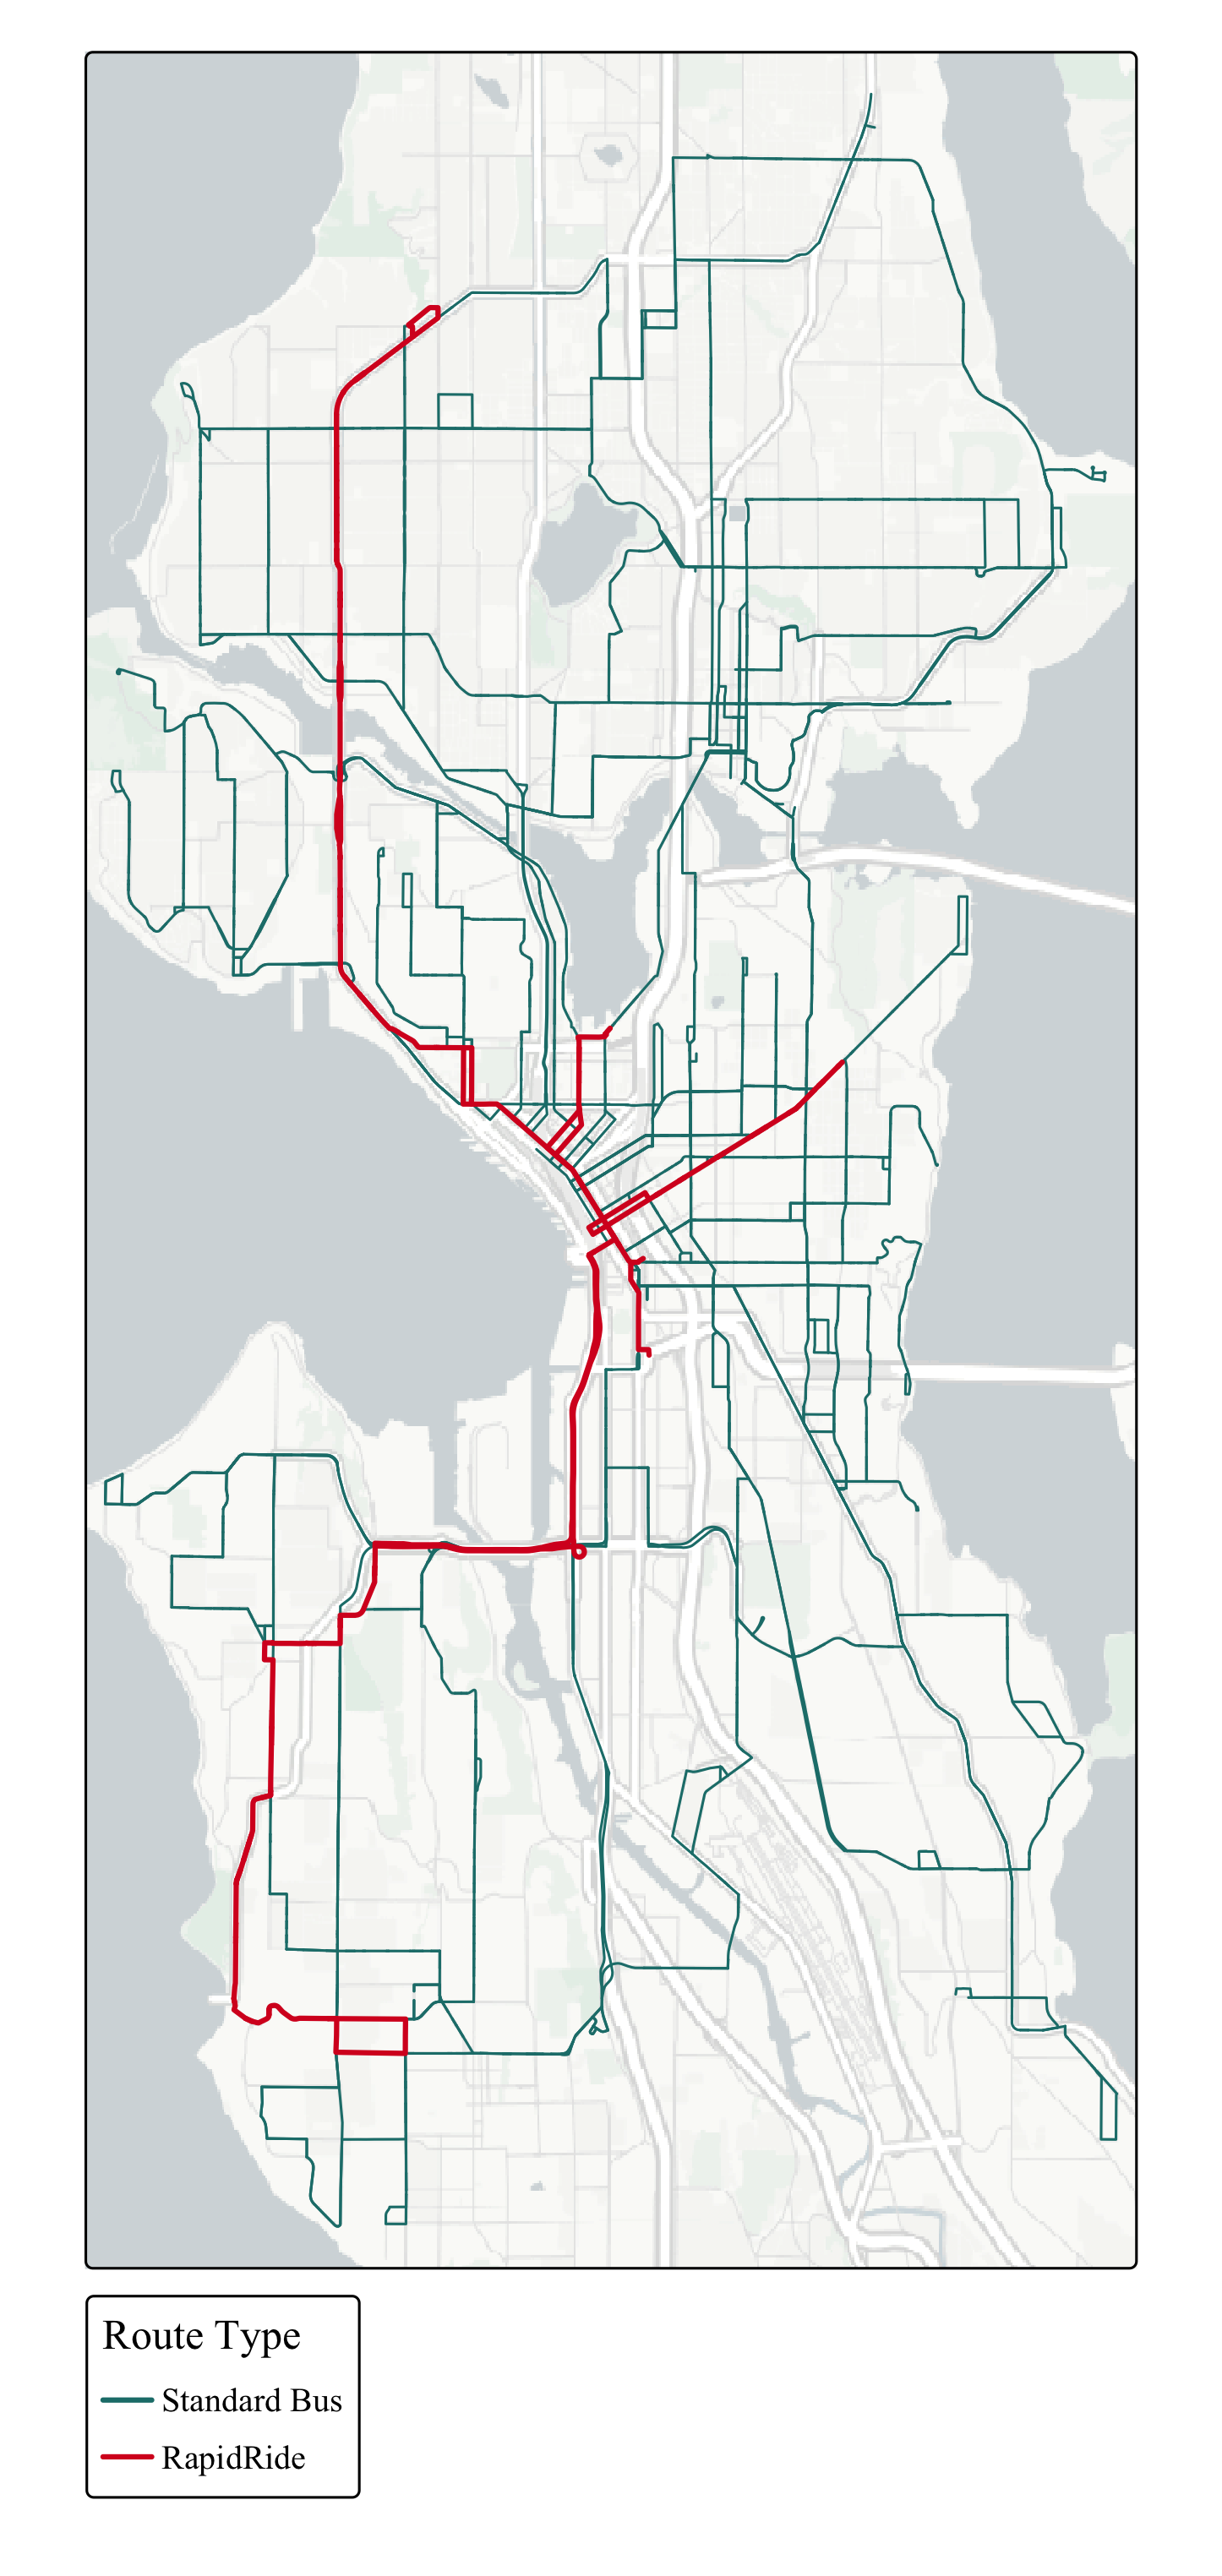
\includegraphics[width=0.45\textwidth]{route_map.png}
  \singlespacing\caption{Map of Standard and RapidRide Bus Service in Seattle, WA. Sources: King County Metro, CartoDB.}
  \vspace{-20pt}
\end{wrapfigure}

The implementation of BRT practices does not happen without significant
investment of time and money, but this investment is far lower than that
required for a major mass transit infrastructure project such as light
rail. As such, BRT is a common choice internationally for developing
cities as a step to formalize informal bus networks with many
independent operators (Muňoz Abogabir \& Paget-Seekins, 2016). That
said, it is also one of the tools that some cities in the United States
have used in an effort to improve municipal transit service.

Seattle introduced the RapidRide program in the early 2010s as an effort
to upgrade busy existing bus routes with some of the principles outlined
above (Consulting, 2019). It is important to note that, despite
characteristics such as off-board fare payment, transit signal priority,
headway management, and some bus-only lanes, RapidRide is not
technically considered to be a full BRT system by the Institute for
Transportation and Development Policy, although the recently-opened G
Line and upcoming H, I, and J Lines are closer to full BRT than previous
lines (Orr, 2024; Transportation and Development Policy (ITDP), 2024).
Rather, one can think of RapidRide as ``BRT-Lite''---an upgrade package
for certain bus routes (often the most busy ones) designed to improve
reliability and frequency of service (Orr, 2024). Figure 1 shows the bus
lines in Seattle, with red lines denoting the RapidRide routes.

As with most public projects, there is a good amount of local discourse
surrounding whether RapidRide is a valuable and worthwhile endeavor for
the City of Seattle and King County Metro, with criticisms ranging from
perceptions of worse service to arguments over whether the investment in
RapidRide could be better used on other transit projects (Fesler, 2024;
Orr, 2024). This research project does not seek to litigate on most of
these issues. The central question to the project remains the somewhat
raw effectiveness of RapidRide---does the RapidRide intervention improve
reliability on a bus route over standard routes?~

\subsection{2.4 The Social Implications of Transit
Performance}\label{the-social-implications-of-transit-performance}

Mass transit, in addition to being a policy needed for sustainability
goals, is a social justice policy. Given that a good, reliable transit
system increases accessibility to the city at large, equitable and
efficient dispersion of quality mass transit options allows for diverse
groups of people to access more areas of the city, opening up job and
recreation opportunities (Covington, 2018). 60\% of urban-area
zero-vehicle households in the United States are low income, which
highlights who is being impacted when public transit is improved (Tomer
\& Puentes, 2011).

This is an issue that is particularly pertinent in Seattle, a city with
a deep history of race-based redlining that carries forward into highly
racially homogenized neighborhoods today (Gregory, 2024). In addition,
Seattle is a highly vertical city--much longer along the North/South
axis than it is wide from West to East. Historically, poorer and
less-white neighborhoods tend to be far North and far South, far away
from many of the urban centers that contain many high-quality job
opportunities and well-funded recreation/entertainment areas (Gregory,
2024).

In essence, the improvement of transit reliability is directly tied to
positive outcomes for individuals across the income and race spectrum.
It has the potential to get people to their jobs on-time on a consistent
basis, open up more job opportunities to people living further outside
the city, and increase accessibility for people and families to quality
recreation and entertainment options.

\section{3. Data Overview}\label{data-overview}

Section 3 will outline the dataset used in this study. The dataset is
not derived from a single source. Rather, it is an amalgamation of data
from several sources, joined at either an individual or group level.
Here, I outline data collection for the outcome variable, absolute
deviation from schedule (AD), and then pivot to a discussion of which
pretreatment covariates were selected and the operationalization of
these variables.

\subsection{3.1 Outcome Data Overview}\label{outcome-data-overview}

The dataset started with the outcome variable, AD. Real-time bus arrival
times are reported by King County Metro via the General Transit Feed
Specification (GTFS), a standard reporting framework for transit
agencies. The real-time GTFS feed is available for public access via an
application programming interface (API). A request can be made to the
API, which will return a list of every stop in the transit network, each
of which has a series of real-time timestamps for recent arrivals at
that stop. These GTFS data are organized in a roughly hierarchical way.
The highest level of this hierarchy is the system as a whole, which can
be split into routes. Routes are the geographical multiline segments on
which trips run. Trips are unique by day, meaning only one instance of a
trip\_id is seen per day. Further, trips are directional, meaning it can
be seen via an indicator variable in the data which direction along a
route the trip travels. Along each trip are stops---pairs of (x, y)
coordinates at which buses stop to load and unload passengers. It is
important to aggregate stops under trips (rather than routes), because
directionality is important. Stop 2 on a route going one direction is
the second-to-last stop going the other direction. So, each row in the
dataset represents a combination of route, trip, and stop identifiers,
which are unique by day. For the data collection in this study, requests
were made to the API on an automated schedule (every 15 minutes from 4am
to 12am, local time, between 1/29/2025 and 3/31/2025). This procedure
resulted in over 4 million rows of observations, from which
approximately 54,000 were sampled for model training and test purposes.
Scheduled arrival times were joined to the dataset by trip\_id/stop\_id
combination. The final outcome variable, AD, is the absolute difference
between the actual arrival time and scheduled arrival time, in seconds.
Seconds as a unit were chosen because they represent the most granular
unit of reporting available. There was an open question as to whether
the outcome variable should discriminate between positive and negative
(i.e., whether the bus arrives early or late) or simply be absolute
deviation (always positive). The choice of AD was made because to use
the positive/negative outcome would have likely required some two-stage
modeling with a step to predict whether the arrival delay would be
positive or negative, and then a step to predict the magnitude. AD is a
simpler construct to model and a bus arriving early or late impacts the
rider in much the same way---it often means increased wait times and the
possibility for a missed transfer.

\subsection{3.2 Covariate Data Overview}\label{covariate-data-overview}

Length of segment and the RapidRide indicator variables are available
via the GTFS static files provided by King County Metro. Length of
segment denotes the distance, in meters, that the bus has traveled
before any given stop. Length of segment is a directional variable and
so was joined to the main dataset by trip\_id. The RapidRide indicator
was assigned based on route\_id. There are three RapidRide routes
present in the dataset, accounting for approximately 16 percent of the
\textasciitilde54,000 sampled observations.

Traffic conditions, another important predictor from the literature,
were somewhat more difficult to translate into the dataset.
Publically-available studies of Seattle traffic either reported traffic
levels as a function of time (e.g., traffic levels by hour, by day) or
as a function of space (e.g., levels of traffic on major arterials), but
not both. Both were added separately to the dataset. Though it is not
necessary to standardize variables for use in a BART, both traffic
datasets were standardized for better interpretability. Rather than
trying to conceptualize how relative vehicle volumes and counts compare
to each other, standardization provides a simple intuition where a value
of 0 means the observation has an average level of traffic relative to
the rest of the city, a 1 indicates the level of traffic is 1 standard
deviation above the mean, and a -1 means the level of traffic is 1
standard deviation below the mean. So, around two-thirds of the data lie
within +/- 1 standard deviation from the mean.

The temporal traffic dataset was available on the Seattle Open Data
Portal. Each row in this dataset represents a study conducted on a
specific date and reports the traffic volume observed during each hour
in the day (data.seattle.gov, 2025). The dataset was filtered to keep
only studies conducted from 2015 onwards and excluded 2020 and 2021 due
traffic disruptions from the COVID-19 pandemic. After these operations,
there were 134,170 rows remaining in the dataset. A traffic volume
number was appended to each entry in the main dataset, corresponding to
the standardized average traffic volume for the weekday and hour that
the entry was from.

Spatial traffic data came from a 2018 study (the most recent such study)
by the Seattle Department of Transportation and contains traffic volume
for each arterial in the city (SDOT, 2018). In order to join these data
to the main dataset, spatial overlays were required. King County Metro
reports the shapefiles for their bus routes, which are multiline strings
(Transit, 2025). One by one, these were overlayed on the spatial traffic
geometry (also multiline strings), which were clipped so that only the
pieces of the arterials that overlapped with the route shape remained.
Then, a weighted average of traffic volume was calculated by multiplying
the traffic volume for each arterial by the proportion of the route line
it covered. Although all bus routes had some level of coverage from the
traffic dataset, not all routes had 100\% coverage. In particular,
routes that run more often on non-arterial streets would have less
coverage. This represents a source of bias in the dataset, but largely a
minor one given that most buses run mostly on arterials.

The next set of predictors are four demographic variables: population
density, ridership percentage, percentage white, and median household
income. Empirical studies have shown that a high volume of ridership
tends to predict decreased bus reliability, as a function of increased
boarding times, thereby increasing dwell time. Regrettably, the
real-time GTFS data used for the outcome variable was not
high-resolution enough to report on dwell times (actual arrival and
departure times were nearly always identical), so it was necessary to
operationalize dwell time in a different way. The American Community
Survey (ACS) 5 year estimates (2019-2023) report the estimated
percentage of each census block group that uses the bus to get to work,
which gives a rough idea of the demand for buses along each route
(Census, 2025). Because transit ridership has been shown to be
positively related to areas of lower income, higher non-white
percentage, and high density, these variables were also included to
better capture variation predicted by high ridership. Again, the route
geometry was used---a half-mile buffer was drawn around each route,
census block groups with over 50\% of their area within the buffer were
selected, and a weighted average ridership percentage was calculated
using block group population as the weighting variable. The half-mile
buffer was selected because it is a commonly used distance threshold for
zoning and policy requirements pertaining to bus lines (Council, 2015).
For computational resource reasons, these variables were calculated at
the full route level, as opposed to the clipping approach used for
spatial traffic.

The final covariates in the dataset are weekday and hour. Weekday takes
the form of an integer with range 1-7, with 1 corresponding to Sunday.
Hour takes the form of an integer with range 1-24. For hour, a 4 denotes
the 4:00 to 4:59 time period. These variables were included as key
structural elements to the data, primarily designed to handle
commuter-based variation in the data that is likely to arise on weekdays
during peak hours.

\section{4. Methods}\label{methods}

Section 4 will review the conceptual background underpinning causal
inference and modeling techniques as they pertain to transit
reliability.

\subsection{4.1 Regression, Causal Inference, and Observational
Studies}\label{regression-causal-inference-and-observational-studies}

This study uses a causal inference framework to study the Seattle's
RapidRide system, as this methodology is widely used to compare
potential outcomes under different applications of some treatment or
intervention (Gelman et al., 2023). In this case, the goal is to compare
potential outcomes for a route that did receive the RapidRide upgrade
``treatment'' versus if the same route had not received the treatment.
Of course, it is impossible to simultaneously observe a route under both
treatment and non-treatment conditions. Further, assignment of the
RapidRide treatment is not random, so the analysis cannot proceed under
the assumptions that accompany a randomized experiment. This lack of
randomness is made clear in materials produced by King County
Metro---routes selected for RapidRide upgrades are among the busiest,
high-frequency routes in the city. They tend to run along busy traffic
corridors and to/through high residential and job density zones (Metro,
2021). This lack of random assignment creates further work and
consideration in the analysis and will be revisited later in this
section. For now, the basic formulation of the causal regression model
is as follows:

\[Eq. 1: Y \sim \beta X + \theta z + \varepsilon\]

In equation 1, \(Y\) represents the outcome (in this case, absolute
deviation from schedule, in seconds, for a given bus at a given bus
stop). \(X\) is the matrix of pretreatment covariates and \(\beta\) is
the vector of coefficients for each of these pretreatment variables.
Finally, \(z\) is the treatment indicator and is equal to 1 for routes
who have had the RapidRide treatment applied to them and 0 for routes
who have not.

Given that these data are observational, the pretreatment covariates
\(X\) are particularly important. The regression must adjust for these,
otherwise the treatment effect is prone to biases resulting from an
imbalanced sample or systematic differences across the treatment and
control groups. In this context, it is probable that average traffic
congestion, for example, is higher along RapidRide routes than among
non-RapidRide routes. The \(\beta X\) term in the regression equation
adjusts for such differences and (theoretically) gives an unbiased
estimate of the difference in outcome y between the control and
treatment groups (henceforth called the treatment effect). Indeed, it
can be shown that, in a hypothetical observational study in which there
is only one pretreatment variable that impacts both the control and
treatment groups, adjustment for this variable will return an unbiased
estimate of the treatment effect (Gelman et al., 2023). Of course, in
the real world there are many pretreatment variables, not all of which
are able to be perfectly accounted for in the analysis. Thus, the
adjustment procedures in the regression can only hope to do as much
adjustment as possible to reduce bias. Further weaknesses of the
regression models is that (a) they assume a linear relationship unless a
different functional form is selected (and the choice of functional form
is rife with opportunities for bias) and (b) they only handle
interactions between variables at a simplistic level. The following
section outlines the model of choice for this study, BARTs, which
addresses these weaknesses and will be compared to a traditional
multivariate linear regression.

\subsection{4.2 Bayesian Additive Regression
Trees}\label{bayesian-additive-regression-trees}

BART is a nonparametric modeling procedure based on ensemble machine
learning methods (Chipman et al., 2010). It provides a nonparametric
regression modeling approach through decision trees, avoids overfitting
(a common issue with decision trees) through a regularization prior,
gives accurate estimates of posterior uncertainty, and elegantly handles
heterogeneous treatment effects (Hill, 2011).\footnote{In a mass
  transit-focused paper, it is worth stating that Bayesian Additive
  Regression Trees (BART) should not be confused with Bay Area Rapid
  Transit (BART).}

Like many Bayesian models, BART uses the Monte Carlo Markov Chain (MCMC)
algorithm, a statistical computing algorithm that draws samples from a
probability distribution through a random walk, iteratively fitting
models. For BARTs, each chain successively builds upon the fit of
previous trees, and overfitting is reduced through the regularization
prior (Chipman et al., 2005).

\subsection{4.3 BARTs for Causal
Inference}\label{barts-for-causal-inference}

The basic regression tree is a simple machine learning model which
creates a series of partitions within the data. The tree begins with a
root node, representing a proper subset of the data. From there, the
tree performs a series of binary splits (each split is called an
interior node), creating a branching series of decision rules that
classify the data. At the bottom of the tree, the terminal nodes (also
known as leaves) represent the final subgroups and give the mean value
of the outcome for observations within these subgroups. A tree is said
to have depth 5 if there are 5 decision rules in the longest path from
the root node to a terminal node. In regression trees, the algorithm
seeks to minimize residual standard error---that is, minimize the
average difference between the value of each terminal node and the
values of the observations within those nodes (Chipman et al., 2010). In
terms of notation, T represents a binary tree consisting of some number
of internal and terminal nodes. \(M = {mu_1, mu_2, …, mu_b}\) describes
the set of parameter values corresponding to each of the \(b\) terminal
nodes in the tree \(T\). A single regression tree can be expressed in
the following way:

\[Eq. 2: Y \sim g(x; T, M) + \varepsilon,\quad \varepsilon \sim N(0, \sigma^2)\]

In equation 2, the outcome \(Y\) is given by the function
\(g(x; T, M)\), which returns a predicted value for an observation with
the set of covariates \(x\). The residual error, \(\varepsilon\), is
assumed to come from a normal distribution with mean \(0\) and standard
deviation sigma. This is analogous to the conditional mean of \(Y\)
given \(x\), \(E(Y | x)\) (Chipman et al., 2010).

A fundamental issue with regression trees is overfitting. Left
unchecked, with no limit on depth, the tree will eventually end up with
n terminal nodes, where n is the number of observations in the sample,
thus fitting the data perfectly. To address this, BARTs use a
sum-of-trees approach combined with a regularization prior (the
``Additive'' and ``Bayesian'' parts of the BART). This approach seeks to
combine a high number of trees while minimizing the amount that each
tree contributes to the overall fit through the regularization prior
(Chipman et al., 2010).

In BARTs, each tree is considered a ``weak learner,'' meaning the
algorithm limits its depth and enforces a strong prior on each terminal
node that shrinks its prediction towards \(0\) (Chipman et al., 2005).
The BART model is the sum of many of these trees, and can be expressed
with similar notation to that of the single tree:

\[Eq. 3: Y = \sum_{j=1}^{m} g(x; T_j, M_j) + \varepsilon, \quad \varepsilon \sim N(0, \sigma^2)\]

The BART approach treats this sum of trees as the model, and uses the
Markov chain Monte Carlo (MCMC) algorithm to iteratively perturb the
weak learning trees to improve the fit (Chipman et al., 2005). These
perturbations can take the form of adding nodes to the tree (growing),
removing nodes from the tree (pruning), or altering a split rule
(changing) (Kapelner \& Bleich, 2016). It is worth mentioning that the
changing perturbation is only applied to singly internal nodes---ones
where both child nodes are terminal nodes (Kapelner \& Bleich, 2016). A
big relative advantage of BARTs over other ensemble regression tree
approaches (e.g., random forest, gradient boosting) is their ability to
produce coherent posterior intervals in addition to point estimates
(Hill, 2011). The algorithm samples from the posterior distribution via
MCMC to quantify uncertainty and behave well. For example, posterior
intervals are likely to be wider for predictions at test points farther
from the training data set (Chipman et al., 2005).

\subsection{4.4 Choice of Estimands and Posterior
Uncertainty}\label{choice-of-estimands-and-posterior-uncertainty}

In cases such as the present research, where multivariate models with
interaction effects and non-parametric approaches are used, regression
coefficients cannot be directly interpreted as the treatment effect.
Rather, an average treatment effect must be calculated by having the
model predict the outcome for a sample set of observations and a
counterfactual set of these observations (Gelman et al., 2023). Because
this study is focused on the effect of the RapidRide intervention, the
sample average treatment effect among the treated (SATT) chosen as the
causal estimand. Calculating the SATT involves filtering the sample to
include only observations that were treated (in this case RapidRide ==
1), and using the model to predict fitted values of AD for each
observation. Then, the treatment variable is set to the counterfactual
(RapidRide == 0) for each of the treated observations, and the model is
used to predict fitted values of AD for each of these counterfactual
observations. Finally, the counterfactual prediction is subtracted from
the factual prediction across each observation and averaged across the
sample, producing the SATT.

A major strength of Bayesian approaches is in achieving posterior
uncertainty in this estimate. Both the multivariate linear and BART
models produce posterior simulation draws (4000 draws for the
multivariate linear and 2000 draws for the BART), representing
uncertainty in the estimates of the model. The procedure above is
repeated for each draw, producing a distribution in individual treatment
effects and, thus, a distribution of SATT estimates. The standard
deviation of these estimates can be examined to see to what degree the
SATT tends to be different from 0 and a confidence interval can be
constructed. In this paper, the standard 95\% confidence interval is
used, in line with most social science literature.

\subsection{4.5 Statistical
Significance}\label{statistical-significance}

Before jumping into the analysis and results, it is important to outline
what constitutes a meaningful result in the context of this study.
Though statistical significance is the status quo when it comes to
quantitative analysis, it has many issues that call into question its
use in the social sciences. It has been shown that statistical
significance is a prerequisite to get research published and that this
(a) leads researchers to make decisions designed to achieve statistical
significance and (b) tends to bias publishable research to reporting
systematically larger effect sizes (Gelman et al., 2023). Further, it is
unrealistic to assume a ``null'' effect (Gelman et al., 2023). In this
context, for example, it does not make sense that the RapidRide upgrade
would cause absolutely no effect on reliability. The effect may be small
(e.g., 5-10 seconds), but this is not a true 0 effect. Rather than
looking for whether the estimated parameters and effect sizes in this
study cross some arbitrary 95\% confidence interval cutoff away from 0
and then deciding that the treatment either works or doesn't, it is
better to simply estimate the effect, examine the associated standard
error, and interpret the results in the light of this information.

\section{5. Analysis and Results}\label{analysis-and-results}

Section 5 will begin with exploration and discussion of descriptive
statistics and assessments of sample balance for causal inference, and
then move to model design and evaluation, in which three models will be
outlined and tested. Finally, SATT estimates and intervals will be
calculated using both Multivariate Linear Regression and BART models.

\subsection{5.1 Descriptive Statistics}\label{descriptive-statistics}

\begin{longtable}[]{@{}
  >{\raggedright\arraybackslash}p{(\columnwidth - 14\tabcolsep) * \real{0.2794}}
  >{\raggedleft\arraybackslash}p{(\columnwidth - 14\tabcolsep) * \real{0.1029}}
  >{\raggedleft\arraybackslash}p{(\columnwidth - 14\tabcolsep) * \real{0.1176}}
  >{\raggedleft\arraybackslash}p{(\columnwidth - 14\tabcolsep) * \real{0.0882}}
  >{\raggedleft\arraybackslash}p{(\columnwidth - 14\tabcolsep) * \real{0.0882}}
  >{\raggedleft\arraybackslash}p{(\columnwidth - 14\tabcolsep) * \real{0.1029}}
  >{\raggedleft\arraybackslash}p{(\columnwidth - 14\tabcolsep) * \real{0.1029}}
  >{\raggedleft\arraybackslash}p{(\columnwidth - 14\tabcolsep) * \real{0.1176}}@{}}
\caption{Descriptive Statistics}\tabularnewline
\toprule\noalign{}
\begin{minipage}[b]{\linewidth}\raggedright
Variable
\end{minipage} & \begin{minipage}[b]{\linewidth}\raggedleft
Mean
\end{minipage} & \begin{minipage}[b]{\linewidth}\raggedleft
Std Dev
\end{minipage} & \begin{minipage}[b]{\linewidth}\raggedleft
Min
\end{minipage} & \begin{minipage}[b]{\linewidth}\raggedleft
25\%
\end{minipage} & \begin{minipage}[b]{\linewidth}\raggedleft
Median
\end{minipage} & \begin{minipage}[b]{\linewidth}\raggedleft
75\%
\end{minipage} & \begin{minipage}[b]{\linewidth}\raggedleft
Max
\end{minipage} \\
\midrule\noalign{}
\endfirsthead
\toprule\noalign{}
\begin{minipage}[b]{\linewidth}\raggedright
Variable
\end{minipage} & \begin{minipage}[b]{\linewidth}\raggedleft
Mean
\end{minipage} & \begin{minipage}[b]{\linewidth}\raggedleft
Std Dev
\end{minipage} & \begin{minipage}[b]{\linewidth}\raggedleft
Min
\end{minipage} & \begin{minipage}[b]{\linewidth}\raggedleft
25\%
\end{minipage} & \begin{minipage}[b]{\linewidth}\raggedleft
Median
\end{minipage} & \begin{minipage}[b]{\linewidth}\raggedleft
75\%
\end{minipage} & \begin{minipage}[b]{\linewidth}\raggedleft
Max
\end{minipage} \\
\midrule\noalign{}
\endhead
\bottomrule\noalign{}
\endlastfoot
RapidRide & 0.16 & 0.37 & 0.00 & 0.00 & 0.00 & 0.00 & 1.00 \\
Absolute Deviation & 210.64 & 233.62 & 0.00 & 64.00 & 147.00 & 276.25 &
3527.00 \\
Distance Traveled & 0.00 & 1.02 & -1.30 & -0.80 & -0.24 & 0.62 & 3.51 \\
Traffic (Day/Hour) & 0.00 & 1.00 & -2.74 & -0.79 & 0.25 & 0.67 & 1.52 \\
Traffic (Location) & 0.01 & 0.99 & -1.51 & -0.53 & -0.15 & 0.45 &
7.81 \\
Population Density & 0.00 & 1.01 & -1.82 & -0.56 & -0.24 & 0.65 &
2.49 \\
Route Ridership & -0.01 & 1.08 & -3.54 & -0.78 & -0.11 & 0.72 & 2.95 \\
Percentage White & 0.04 & 0.97 & -2.40 & -0.35 & 0.20 & 0.70 & 2.04 \\
Median HHI & 0.05 & 0.99 & -2.03 & -0.76 & 0.33 & 0.79 & 1.68 \\
Weekday & 3.79 & 1.93 & 1.00 & 2.00 & 4.00 & 5.00 & 7.00 \\
Hour & 14.56 & 5.08 & 1.00 & 10.00 & 15.00 & 19.00 & 24.00 \\
\end{longtable}

The exploratory data analysis process begins with an overview of the
data, variables, and their characteristics. Table 1 contains basic
descriptive statistics across the outcome, treatment, and pre-treatment
variables in the sample.

RapidRide has a mean of 0.16, indicating that the sample is comprised of
16\% of observations occurring at stops along RapidRide routes and 85\%
of observations occurring along non-RapidRide routes. This distribution
is the result of some oversampling of RapidRide observations, as natural
incidence rates of RapidRide observations were closer to 8\%. This
allows the model more information when it comes to estimating the
treatment effect but does not grossly overstate the incidence of
RapidRide routes in the city, which would be the case if the sampling
was done at a 50/50 level.

The average AD for observations in the sample is 210 seconds. In other
words, the average bus arrival is 3.5 minutes away from its scheduled
arrival time. It is important to note that the median observation is 147
seconds, so the distribution is affected by some extremely late or early
bus arrivals (the greatest of which is nearly 3600 seconds, or about an
hour). The standard deviation of 233 seconds indicates very high
variability for these outcomes. Though some observations close to the
maximum could be considered outliers by the classical definition of
\(mean + 3*sd\), they were not removed in order to preserve the accuracy
of the sample--sometimes buses run an hour late and it would be a
mistake to exclude that information from the analysis.

The following variables were centered and standardized: Distance
Traveled, Traffic (Day/Hour), Traffic (Location), Population Density,
Route Ridership, Percentage White, and Median HHI. Each of these
variables has mean approximately equal to 0 and standard deviation
approximately equal to 1, though these are slightly changed as a result
of the RapidRide oversampling.

Finally, the roughly similar values of mean and median for Weekday and
Hour indicate fairly even distributions of observations across day and
hours. For hours, though, the mean being a bit above 12 (the presumed
mean), indicates a lack of observations in the early hours of the
morning. This is expected since King County Metro does not run buses
between around midnight and 4am.

\begin{longtable}[]{@{}rrrr@{}}
\caption{Balance Statistics for Causal Inference}\tabularnewline
\toprule\noalign{}
Treat & Control & Difference & Ratio \\
\midrule\noalign{}
\endfirsthead
\toprule\noalign{}
Treat & Control & Difference & Ratio \\
\midrule\noalign{}
\endhead
\bottomrule\noalign{}
\endlastfoot
199.04 & 212.93 & -13.89 & 1.10 \\
0.07 & -0.01 & 0.08 & 0.84 \\
0.01 & 0.00 & 0.01 & 0.97 \\
0.06 & -0.01 & 0.07 & 1.20 \\
-0.04 & 0.01 & -0.05 & 0.96 \\
-0.08 & 0.01 & -0.09 & 0.52 \\
0.48 & -0.05 & 0.53 & 4.33 \\
0.60 & -0.06 & 0.66 & 1.46 \\
3.68 & 3.81 & -0.12 & 1.03 \\
14.27 & 14.62 & -0.35 & 1.00 \\
\end{longtable}

Beyond simple descriptives, it is important to assess balance when
dealing with causal inference: do the characteristics of the control and
treatment groups looks roughly similar? Table 2 compares the raw means
of the two samples in the ``treat'' and ``control'' columns, along with
the difference. Further, the ``ratio'' column provides a quick
comparison---a value of 1 indicates perfect balance between the
treatment and control. The ratio for many covariates is near 1,
indicating reasonable balance. There are three variables of slight
concern. Route Ridership demand is lower for RapidRide routes than for
non-RapidRide routes, and RapidRide routes tend to run though areas that
are much whiter and somewhat higher income than non-RapidRide routes.
These three variables are correlated with each other (see Figure 2), so
imbalance across all three of them is unsurprising. Adjustment within
the regression and BART models is designed to account somewhat for these
differences, but they do point to possible reasons that the raw
difference between the treatment and control may be misleading. Finally,
Figure 2 contains a correlation plot for each of the treatment, outcome,
and pre-treatment variables. Absolute Deviation is slightly correlated
with a number of predictors.

\begin{figure}

{\centering 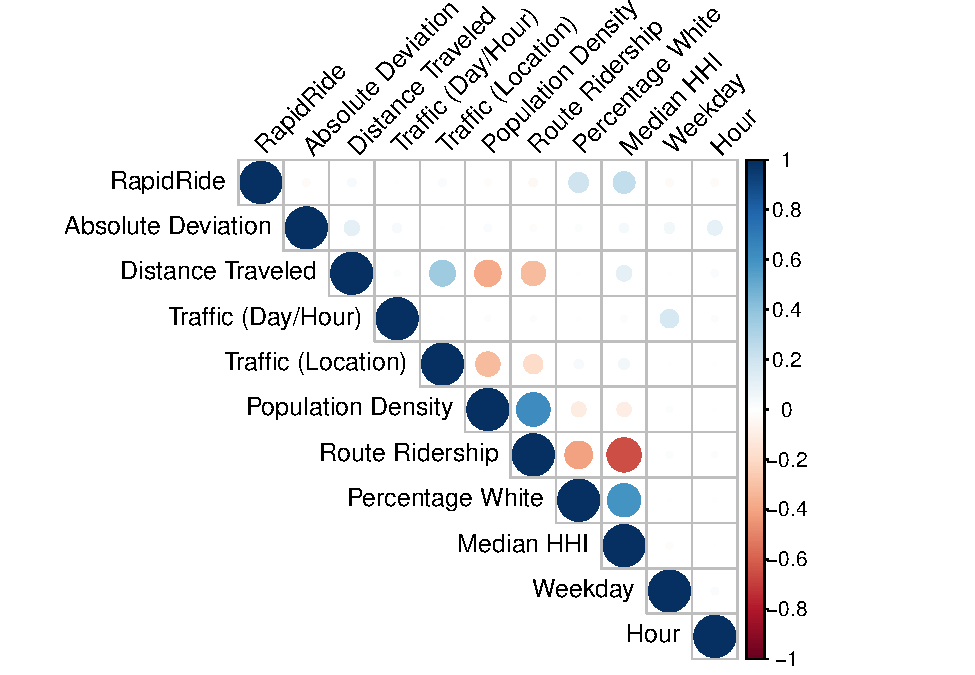
\includegraphics[width=0.6\linewidth]{figures/unnamed-chunk-9-1} 

}

\caption{Correlation Plot}\label{fig:unnamed-chunk-9}
\end{figure}

\subsection{5.2 Model Design and
Evaluation}\label{model-design-and-evaluation}

The present study considers three models: a simple binary linear
regression of AD on RapidRide treatment, a multivariate linear
regression of AD on RapidRide treatment and pre-treatment variables,
with interactions, and a non-parametric BART model. Section 5.2 will
give an overview of the model specifications, assessment of model
performance, and a discussion as to which models will be used in the
final analysis.

The simple linear regression of AD on the binary RapidRide treatment
variable, formalized in equation 4, produces a coefficient that may be
interpreted as the difference in means between the control and treatment
groups.

\[Eq. 4: AD \sim \theta*RapidRide + \varepsilon\]

As discussed earlier, though, in this observational setting it is key to
adjust for pre-treatment variables within the regression model in an
effort to account for bias and systematic differences between the
groups. Additionally, it is reasonable to think that the RapidRide
treatment may be heterogeneous for different subgroups of the data. For
example, perhaps it is more effective on certain days or hours, or in
areas of relatively higher traffic. Finally, in a simplistic effort to
capture possible nonlinearities within the data, two interaction terms
between pre-treatment variables were included: distance traveled x
traffic (day/hour) and distance traveled x traffic (location), with the
hypothesis that traffic effects get more pronounced the further the bus
has to go. As such, equation 5 formalizes the regression equation.

\[
\begin{aligned}
Eq. 5: AD &= \beta_0 + \beta_1 RapidRide + \beta_2 X + \beta_3 (RapidRide \times X_{subset}) + \beta_4 (X_{interaction}) + \varepsilon \\
\varepsilon &\sim N(0, \sigma^2) \\
X_{subset} &= (Weekday,\, Hour,\, Traffic\,(Location),\, Traffic\,(Day/Hour),\, RouteRidership) \\
X_{interaction} &= Traffic(Location) \times Traffic(Day/Hour) + \\
&\quad DistanceTraveled \times Traffic(Location) + \\
&\quad DistanceTraveled \times Traffic(Day/Hour)
\end{aligned}
\]

Finally, the specification for the BART model. As discussed previously,
one of the advantages of the BART model is its ability to find
nonlinearities within the data and look for heterogeneous treatment
effects by subgroup. The specification of the BART model is
straightforward, as can be seen in equation 6.

\[Eq. 6: AD \sim BART(RapidRide + X)\]

To compare the fit of the BART model to those of the linear regression
models, fitted predictions be compared to observed data to calculate the
Residual Mean Squared Error (RMSE), where lower RMSE indicates a better
fit. Table 5 computes and compares the RMSE for a holdout test set of
50,000 observations. Though the values are relatively similar, there is
a clear improvement between the Binary Linear and Multivariate Linear
models, as well as the Multivariate and BART models.

\begin{longtable}[]{@{}lr@{}}
\caption{RMSE by Model}\tabularnewline
\toprule\noalign{}
Model & RMSE \\
\midrule\noalign{}
\endfirsthead
\toprule\noalign{}
Model & RMSE \\
\midrule\noalign{}
\endhead
\bottomrule\noalign{}
\endlastfoot
Binary Linear & 236.36 \\
Multivariate Linear & 233.11 \\
Bayesian Additive Regression Trees & 225.40 \\
\end{longtable}

As a final aspect to the model evaluation stage, it is important to
examine the posterior residual sigma values for each chain in the BART
Model. When the model is well-specified and the algorithm is able to
converge on a parameters with relative ease, each of the four chains
mixes well with the others, producing similar values of sigma. When the
model is not well-specified, the chains often diverge and produce
substantially different values of sigma, the standard deviation of the
error term (Vehtari et al., 2021). Divergence wastes MCMC chain
iterations and can lead to bias in the output of the model. There are
two ways to evaluate the model on this front. First, one can simply plot
the values of sigma over the iterations of each chain and visually
inspect the pattern to see if mixing has occurred. Second, one can
calculate r-hat, a metric that compares the variation in sigma within
each chain to the variation in sigma across all the chains. A value of 1
is ideal, and a value above 1 indicates that some level of poor mixing
has occurred (a value below 1 is not possible). Standard recommendation
is that a r-hat value of less than 1.1 is ideal (Vehtari et al., 2021).
Figure 3 presents a graph of Sigma Posterior Samples by Chain, along
with the estimated r-hat of 1.18. Admittedly, this value of r-hat is
above usual recommendations, indicating that additional work should be
done to better specify the model or specify better priors to avoid bias.
That being said, the later estimates produced by the model are fairly
coherent and time in a master's thesis is limited, so the research
proceeds with the caveat that the model is sub-optimal.

\begin{figure}

{\centering 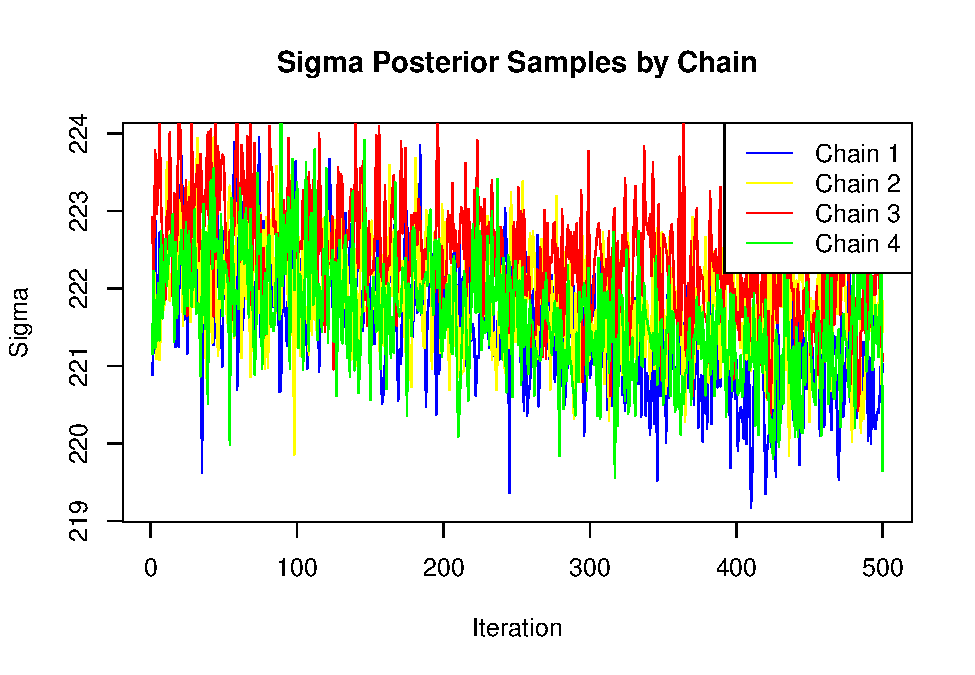
\includegraphics[width=0.6\linewidth]{figures/unnamed-chunk-11-1} 

}

\caption{R-Hat = 1.18}\label{fig:unnamed-chunk-11}
\end{figure}

\subsection{5.3 Results}\label{results}

Section 5.3 will begin with a comparison of results for the two
regression models. The BART, being nonparametric in nature, returns no
regression coefficients and, thus, cannot be compared directly to the
regression models in this way. Instead, the BART model and the
multivariate linear model will each be used to compute the sample
average treatment effect among the treated (SATT), which does allow for
a comparison between the two types of model.

\subsubsection{5.3.1 Regression Results}\label{regression-results}

\begingroup\fontsize{9}{11}\selectfont

\begin{longtable}[t]{>{\raggedright\arraybackslash}p{2.5cm}>{\raggedleft\arraybackslash}p{2cm}>{\raggedleft\arraybackslash}p{2cm}>{\raggedleft\arraybackslash}p{2cm}>{\raggedleft\arraybackslash}p{2cm}}
\caption{\label{tab:unnamed-chunk-12}Linear Regression Coefficients}\\
\toprule
Parameter & Estimate (Binary) & SE (Binary) & Estimate (Multivariate) & SE (Multivariate)\\
\midrule
Intercept & 212.98 & 1.11 & 216.70 & 1.15\\
RapidRide & -13.94 & 2.74 & -105.32 & 39.29\\
Distance Traveled & NA & NA & 36.09 & 1.13\\
Traffic (Day/Hour) & NA & NA & 8.84 & 1.10\\
Traffic (Location) & NA & NA & -6.77 & 1.16\\
\addlinespace
Population Density & NA & NA & 19.08 & 1.66\\
Route Ridership & NA & NA & -7.66 & 2.56\\
Percentage White & NA & NA & 0.08 & 1.43\\
Median HHI & NA & NA & 5.46 & 1.92\\
\bottomrule
\end{longtable}
\endgroup{}

Table 4 reports the estimated coefficients for each variable, along with
standard error, for the two regression models. Although statistical
significance is not a core outcome of interest for this study,
multiplying the standard error by 2 provides a reasonable estimate of
the upper/lower bounds of a 95\% confidence interval. First, it is clear
that both models estimate a negative relationship between RapidRide and
AD, indicating that RapidRide routes are, on average, more reliable.
Further, most predictors in the multivariate model have coefficients
that are quite a bit larger than their standard errors, meaning the
model estimates they do have an effect on the outcome. Though it is
possible to go through the interaction effects and determine the
estimated effect of the RapidRide treatment for each combination of
variables, it is simpler to compute the SATT, which will be done in the
next section.

\subsubsection{5.3.2 Sample Average Treatment Effect among the Treated
(SATT)}\label{sample-average-treatment-effect-among-the-treated-satt}

Because of the less-than-ideal r-hat values for the BART model and the
relative similarity between the RMSE values for the BART model and
multivariate linear models, both will be used to calculate SATT
estimates. The estimates, along with their distributions, can be
examined comparatively to get a better idea of what each model is saying
about the research question and, together, they should give a decent
picture of the underlying effect.

\begin{longtable}[]{@{}rrr@{}}
\caption{SATT, 95\% Confidence Interval}\tabularnewline
\toprule\noalign{}
Estimate & Lower95 & Upper95 \\
\midrule\noalign{}
\endfirsthead
\toprule\noalign{}
Estimate & Lower95 & Upper95 \\
\midrule\noalign{}
\endhead
\bottomrule\noalign{}
\endlastfoot
-48.70 & -84.05 & -11.90 \\
-15.36 & -24.25 & -6.68 \\
\end{longtable}

To calculate the SATT and include its uncertainty, the dataset was
filtered to only include treated observations (RapidRide == 1),
resulting in n = 8981 treated observations. Then, the dataset was copied
and all of the 1s in the RapidRide column were flipped to 0. This
provides the counterfactual---two observations that are identical across
all pretreatment variables but that differ on the treatment variable.
Each model is then used to estimate fitted predictions for each
observation. It is important to note that both models have several
thousand posterior sampling draws, so they produce several thousand
fitted values per observation. To be precise, the multivariate linear
regression produces 4000 estimates per observation and the BART model
produces 2000 estimates per observation. These estimates provide the
posterior uncertainty associated with the SATT estimates and allow for
the construction of confidence intervals. Once the predictions are made,
the counterfactual predictions are subtracted from the factual
predictions to produce individual estimates of the treatment effect for
each observation across each simulation draw. Then, the individual
estimates are averaged for each simulation draw, producing 4000
estimated SATTs for the multivariate linear model and 2000 estimated
SATTs for the BART model. These represent the estimated distribution of
the SATT. Table 5 provides the estimated median SATT for each model,
along with an upper and lower bound consistent with a 95\% confidence
interval. In this case, a negative estimate indicates a decrease in AD
and an improvement in reliability as a result of the RapidRide
treatment. Further, both models produce upper bounds that are still
negative, indicating high likelihood that the true value of the average
treatment effect among the treated is negative.

It is interesting, though, to examine the distributions of the estimates
of the SATT between the two models. Figure 4 present density plots of
the two distributions, with the BART distribution in blue and the
multivariate linear distribution in red. Both look normally distributed,
which is expected given that both models rely on the assumption of
normally-distributed error terms, but it is clear that the BART
estimates are much more variable than the multivariate linear. Given
that BARTs are designed to capture complex interactions and
nonlinearities within the data, this additional uncertainty is expected.
The more important takeaway is the relative agreement of the two models
that the effect of the RapidRide intervention is generally an
improvement to reliability.

\begin{figure}

{\centering 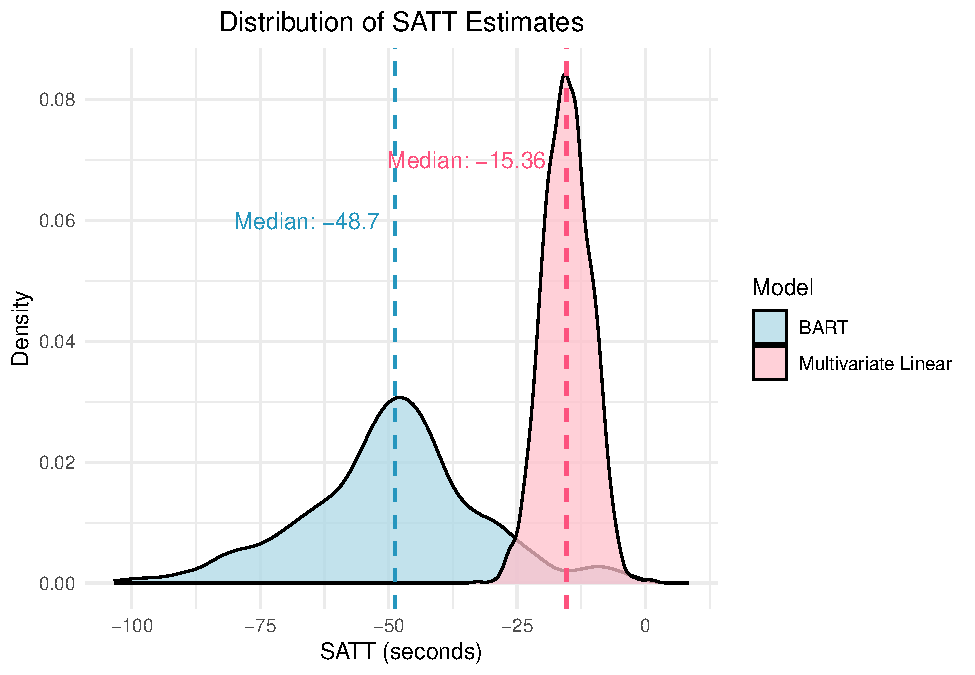
\includegraphics[width=0.7\linewidth]{figures/unnamed-chunk-14-1} 

}

\caption{The two models not only differ in their mean estimate of the sample average treatment effect, they also estimate different variability within these estimates.}\label{fig:unnamed-chunk-14}
\end{figure}

\subsubsection{5.3.3 Model Comparison: Subgroup
Estimates}\label{model-comparison-subgroup-estimates}

In addition to the single estimate of SATT, it is interesting to examine
differing effects for various subgroups of the data. Not only does it
provoke interesting discussion about where and when the RapidRide
intervention is effective, but it also demonstrates further differences
between the models used. For this example, the SATT is calculated
separately for each hour of the day in the dataset. There are no
observations for hours 2 or 3, so this results in 22 distributions of
the SATT for each model. Figure 5 plots these estimates to show the
comparison between the BART and multivariate linear models. The circles
represent the median estimate, and the error bars represent a 95\%
confidence interval for the distribution.

The most obvious difference between the models is the variability of the
estimates. Using the linear regression model alone, there would be
strong evidence that the treatment effect is more pronounced between the
hours of 6 and 10, and that it disappears or even changes sign in the
afternoon and evening hours. Conversely, the BART model shares
information between subgroups, and partially-pools the estimates,
resulting in much more stable estimates of the treatment effect. While
it seems unlikely that the treatment effect of the RapidRide
intervention changes sign for the last few hours of the day, it is not
inconceivable. This is somewhat corroborated by the BART estimates---the
95\% confidence intervals for the afternoon and evening hours often
include 0. Another interesting difference is that the confidence
intervals for the multivariate linear model are smaller than the BART
for subgroups with larger samples, but the opposite is true for hours
with low amounts of observations, such as 1am and 4am. This is, again,
due to partial pooling. That said, rather than making a strict value
judgement about which model is better than the other, it is likely a
better strategy to synthesize what each model says and proceed as if
both provide insights.

\begin{figure}

{\centering 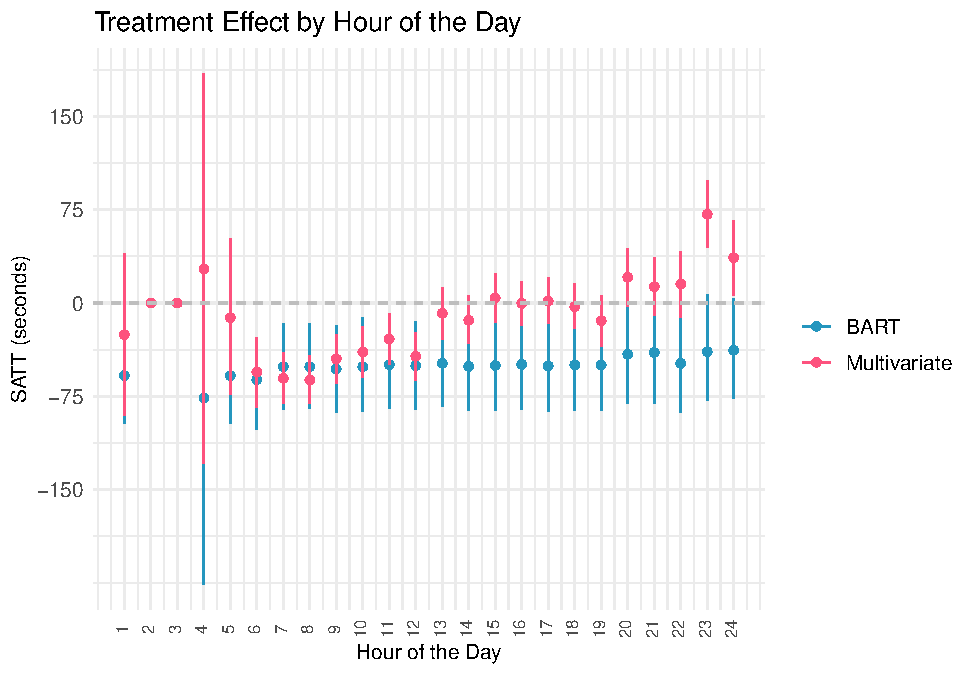
\includegraphics[width=0.7\linewidth]{figures/unnamed-chunk-15-1} 

}

\caption{The models vary in their estimated treatment effect by hour, with the BART estimating more homogeneous effects, while the multivariate linear model's estimates are more variable with greater variation in their uncertainty.}\label{fig:unnamed-chunk-15}
\end{figure}

\section{6. Discussion}\label{discussion}

\subsection{6.1 Implication for Policy}\label{implication-for-policy}

At a very basic level, these results are a good sign for the RapidRide
system. Though it has many stated goals, an improvement in reliability
of service is a fundamental win for the system. That being said, the
magnitude of the improvement is a question that came up time and time
again through the analysis of these results. Take, for example, the
multivariate linear results, which point to an effect of about 15
seconds. Is this worth it? While certainly better than no change or a
decrease in reliability, it is difficult to say whether an average
improvement of 15 seconds is a worthwhile investment of several million
dollars. On the other hand, the BART estimate of almost 60 seconds seems
to be a more enticing effect. To ground these numbers in reality, a 2021
report from King County Metro entitled ``Transit Speed \& Reliability
Guidelines and Strategies'' highlights that buses arriving more than a
minute early or more than 5-and-a-half minutes late violate the rules of
``on-time performance'' for standard bus routes and that the goal for
RapidRide buses is arrival within 2 minutes on either side of the
scheduled arrival time (Metro, 2021). In the context of these figures,
the nearly 60-second average improvement seen for the RapidRide
intervention does appear to be impactful relative to existing goals.

Moving beyond simple reliability, mass transit is an important social
equity tool that should be used by the city to break down boundaries
between neighborhoods in Seattle, a city with a long history of
redlining and racial/socioeconomic segregation by neighborhood. A 2019
King County Metro report outlines recommendations from the Mobility
Equity Cabinet and identifies increasing and improving bus service in
areas of high density and high proportion low-income and people of color
as their top recommendation for investment (Metro, 2019). Given that
transit should be used to increase access to the wider city from
neighborhoods of a diverse range, this evidence that the RapidRide
system functions well is a signal that King County and the City of
Seattle should continue to fund the program. As was clear from the
analysis of balance between RapidRide and non-RapidRide routes, the
RapidRide routes within the city disproportionately lie in areas of
higher income and higher percentage white residents. Future routes
should focus on areas of lower wealth and higher proportions of minority
residents.

Another theme that arose through the project was the idea of
granularity. In local matters especially, every dollar counts. Policy
decisions may start at the 30,000-foot, strategic priority level, but
they filter down into fundamental, small-scale decisions about
allocation of time and funding to extremely specific areas. This is a
major weakness of a lot of traditional (i.e., non-Bayesian, non-pooling)
regression methods---when the subgroups get really small, the
uncertainty gets really big. There is a common heuristic that you need
around 16x the sample size to effectively estimate an interaction effect
as compared to a main effect, and this heuristic only refers to a single
interaction, not to speak of varying treatment effects by hour of the
day, day of the week, and on a specific bus route. Through
partial-pooling and Bayesian approaches, these subgroups can at least be
estimated with a higher degree of precision, even if the smallest
subgroups are pooled in towards the overall mean. BART models are
designed to handle this sort of thing, while providing the ability to
estimate non-linearities easily, making them a really valuable tool for
causal inference moving forward.

\subsection{6.2 Limitations}\label{limitations}

Modeling is defined in large part by its limitations, and this project
is no different. Broadly, the limitations of the project can be placed
into three categories: data quality, generalizability, and model
specification.

Some of the data for this project is extremely accurate. The GTFS
real-time feeds and data on route distances/RapidRide treatment are
highly accurate and suffer from essentially no missingness whatsoever.
The main data quality issue for the dataset is in the application of
covariates to individual observations. First, an ideal dataset would
include real-time traffic estimates for each observation, rather than
aggregate estimates for time and place based on historical data. This
change, simple to outline and difficult to actually implement, would
likely improve the predictive accuracy of the model by a large margin.
Additionally, the operationalization of the ridership variable is
imperfect---the census variables would be better replaced by route-level
ridership data combined with daily ridership numbers, in an ideal world.
Further, the variable set is likely insufficient to satisfy the
assumption that all confounding covariates are adjusted for within the
model.

Further, the inferences associated with this study are only truly
generalizable to the time period in which the data was collected (the
first few months of 2025). It may be reasonable to generalize the
findings to other months and years, but it is hard to say this without
additional evidence.

Lastly, there are the previously outlined issues with model
specification. The BART model did not mix particularly well, and it is
likely that the addition of some priors or some other model
specification would improve the fit and, thus, the inference.
Additionally, there are more complex versions of the BART model that
allow for concretely defined hierarchical structure to the data (Dorie
et al., 2022). These data are structured by day and hour, as well as by
stop-trip-and-route. Accounting for these explicitly in a multilevel
structure and then using a BART term for the remaining covariates would
likely provide better causal inference than the current models.

\subsection{6.3 Future Directions}\label{future-directions}

With the limitations above addressed, this model becomes a powerful tool
for public policy researchers and decision-makers. The first future
direction for this research is a wider-scale study involving samples
from throughout a year, with further adjustment for seasonal/holiday
trends. Further, there are additional RapidRide bus routes outside of
the Seattle city limits. While all routes outside the city limits
(RapidRide and otherwise) were omitted from the current research because
they lacked spatial traffic data, a more inclusive study would provide
better inference for the project as a whole.

A huge possibility for this research is in cross-city comparison. Many
cities have bus rapid transit systems, and inferences across cities
could be combined for a better understanding of the intervention as a
whole. The standardized GTFS structure of real-time transit data used in
cities across the US and around the world makes data comparable across
cities, which is a big boon to modeling. Further, one weakness of the
present research is that it fails to discriminate between different
aspects of the RapidRide intervention---that is, it is unknown which
part(s) of the intervention is responsible for the positive impact on
reliability. Because many cities implement BRT differently, it may be
possible to subclassify BRT programs based on the specifics of their
upgrades, and isolate which of traffic signal priority, decreased dwell
times, headway management, etc. are most effective in improving transit
reliability.

Lastly, the SATT estimates for this study were calculated on RapidRide
routes, but the procedure can be reversed, so the counterfactual turns
non-RapidRide routes into RapidRide ones. BARTs are well-suited to this
task as well---they account for uncertainty when balance and support
between the treatment and control groups are not good, meaning inference
for control observations without solid support and balance from the
treatment group would have more uncertainty associated with them. This
could be used by policymakers to identify routes with the greatest
potential for reliability improvements, alongside traditional indicators
that make a route attractive for an upgrade.

\section{7. Conclusion}\label{conclusion}

Causal inference in observational settings is hard, and the case of
RapidRide in Seattle is no different. The treatment is demonstrably
applied in a non-random way, creating a fundamental violation of the
principle of ignorability. Further, it is more interesting to examine
the current state of the program, rather than trying to achieve a
pre-post setup when the intervention was implemented, given that it
changes and evolves over time. So, the question of what effect the
RapidRide program has on the reliability of a bus route in 2025 is a
question that can only be answered with modeling and adjustment. BARTs
and multivariate linear regression both provide solutions, and the
inferences that come from these models can help inform policymakers as
to whether the intervention is successful. The present study provides an
initial result that the RapidRide intervention has the intended effect
on reliability and reduces absolute deviation from schedule on a bus
route by an average of nearly 90 seconds per minute. Further results in
subgroups provide future areas for research---granular understanding of
these patterns is paramount to better-allocated spending on mass transit
in the future.

\singlespacing

\newpage

\section{8. References}\label{references}

\phantomsection\label{refs}
\begin{CSLReferences}{1}{0}
\bibitem[\citeproctext]{ref-anderson_racialethnic_2021}
Anderson, K. F., \& Galaskiewicz, J. (2021). Racial/{Ethnic}
{Residential} {Segregation}, {Socioeconomic} {Inequality}, and {Job}
{Accessibility} by {Public} {Transportation} {Networks} in the {United}
{States}. \emph{Spatial Demography}, \emph{9}(3), 341--373.
\url{https://doi.org/10.1007/s40980-021-00093-8}

\bibitem[\citeproctext]{ref-antipova_accessibility_2020}
Antipova, A., Sultana, S., Hu, Y., \& Rhudy, J. P. (2020). Accessibility
and {Transportation} {Equity}. \emph{Sustainability}, \emph{12}(9),
3611. \url{https://doi.org/10.3390/su12093611}

\bibitem[\citeproctext]{ref-us_census_american_2025}
Census, U. (2025). \emph{American {Community} {Survey} ({ACS})}.
\url{https://www.census.gov/programs-surveys/acs}

\bibitem[\citeproctext]{ref-chen_bayesian_2024}
Chen, X. (2024). \emph{Bayesian inference and forecasting methods in
public transit systems}.

\bibitem[\citeproctext]{ref-chipman_bart_2005}
Chipman, H. A., George, E. I., \& McCulloch, R. E. (2005). \emph{{BART}:
{Bayesian} {Additive} {Regression} {Trees}}.

\bibitem[\citeproctext]{ref-chipman_bart_2010}
Chipman, H. A., George, E. I., \& McCulloch, R. E. (2010). {BART}:
{Bayesian} additive regression trees. \emph{The Annals of Applied
Statistics}, \emph{4}(1). \url{https://doi.org/10.1214/09-AOAS285}

\bibitem[\citeproctext]{ref-sam_schwartz_consulting_bus_2019}
Consulting, S. S. (2019). \emph{Bus {Reliability}}.

\bibitem[\citeproctext]{ref-puget_sound_regional_council_transit-supportive_2015}
Council, P. S. R. (2015). \emph{Transit-{Supportive} {Densities} and
{Land} {Uses}}.

\bibitem[\citeproctext]{ref-covington_overcoming_2018}
Covington, K. L. (2018). Overcoming {Spatial} {Mismatch}: {The}
{Opportunities} and {Limits} of {Transit} {Mode} in {Addressing} the
{Black}--{White} {Unemployment} {Gap}. \emph{City \& Community},
\emph{17}(1), 211--235. \url{https://doi.org/10.1111/cico.12278}

\bibitem[\citeproctext]{ref-dataseattlegov_traffic_2025}
data.seattle.gov. (2025). \emph{Traffic {Count} {Studies} by {Hour}
{Bins}}.
\url{https://catalog.data.gov/dataset/traffic-count-studies-by-hour-bins}

\bibitem[\citeproctext]{ref-diab_bus_2015}
Diab, E., Bertini, R., \& El-Geneidy, A. (2015). \emph{Bus transit
service reliability: {Understanding} the impacts of overlapping bus
service on headway delays and determinants of bus bunching}.

\bibitem[\citeproctext]{ref-dorie_stan_2022}
Dorie, V., Perrett, G., Hill, J. L., \& Goodrich, B. (2022). Stan and
{BART} for {Causal} {Inference}: {Estimating} {Heterogeneous}
{Treatment} {Effects} {Using} the {Power} of {Stan} and the
{Flexibility} of {Machine} {Learning}. \emph{Entropy}, \emph{24}(12),
1782. \url{https://doi.org/10.3390/e24121782}

\bibitem[\citeproctext]{ref-renne_taking_2013}
Dutta, P. K. (2013). Taking the {Car} out of {Carbon}. In J. L. Renne \&
B. Fields (Eds.), \emph{Transport {Beyond} {Oil}} (pp. 126--140). Island
Press/Center for Resource Economics.
\url{https://doi.org/10.5822/978-1-59726-242-2_8}

\bibitem[\citeproctext]{ref-fesler_case_2024}
Fesler, S. (2024). \emph{The {Case} {Against} {RapidRide} and {For}
{Funding} {Massive} {Transit} {Service} {Expansion} {Now}}.
\url{https://www.theurbanist.org/2024/02/29/the-case-against-rapidride-and-for-funding-massive-transit-service-expansion-now/}

\bibitem[\citeproctext]{ref-gelman_regression_2023}
Gelman, A., Hill, J., \& Vehtari, A. (2023). \emph{Regression and
{Other} {Stories}}.

\bibitem[\citeproctext]{ref-gregory_homes_2024}
Gregory, J. (2024). Homes for {Some}: {Seattle}'s {History} of {Housing}
and {Racial} {Exclusion}. \emph{Pacific Northwest Quarterly},
\emph{115}(1), 26--36.
\url{http://ezproxy.cul.columbia.edu/login?url=https://search.ebscohost.com/login.aspx?direct=true&db=31h&AN=182205574&site=ehost-live&scope=site}

\bibitem[\citeproctext]{ref-hagerstrand_what_1970}
Hägerstrand, T. (1970). What about people in regional science.
\emph{Transport Sociology: Social Aspects of Transport Planning},
143--158.

\bibitem[\citeproctext]{ref-handy_is_2020}
Handy, S. (2020). Is accessibility an idea whose time has finally come?
\emph{Transportation Research Part D: Transport and Environment},
\emph{83}, 102319. \url{https://doi.org/10.1016/j.trd.2020.102319}

\bibitem[\citeproctext]{ref-hansen_how_1959}
Hansen, W. G. (1959). How {Accessibility} {Shapes} {Land} {Use}.
\emph{Journal of the American Institute of Planners}, \emph{25}(2),
73--76. \url{https://doi.org/10.1080/01944365908978307}

\bibitem[\citeproctext]{ref-hill_bayesian_2011}
Hill, J. L. (2011). Bayesian {Nonparametric} {Modeling} for {Causal}
{Inference}. \emph{Journal of Computational and Graphical Statistics},
\emph{20}(1), 217--240. \url{https://doi.org/10.1198/jcgs.2010.08162}

\bibitem[\citeproctext]{ref-huang_bus_2021}
Huang, Y. P., Chen, C., Su, Z. C., Chen, T. S., Sumalee, A., Pan, T. L.,
\& Zhong, R. X. (2021). Bus arrival time prediction and reliability
analysis: {An} experimental comparison of functional data analysis and
{Bayesian} support vector regression. \emph{Applied Soft Computing},
\emph{111}, 107663. \url{https://doi.org/10.1016/j.asoc.2021.107663}

\bibitem[\citeproctext]{ref-kapelner_bartmachine_2016}
Kapelner, A., \& Bleich, J. (2016). \textbf{bartMachine} : {Machine}
{Learning} with {Bayesian} {Additive} {Regression} {Trees}.
\emph{Journal of Statistical Software}, \emph{70}(4).
\url{https://doi.org/10.18637/jss.v070.i04}

\bibitem[\citeproctext]{ref-levinson_towards_2020}
Levinson, D., \& Wu, H. (2020). Towards a general theory of access.
\emph{Journal of Transport and Land Use}, \emph{13}(1), 129--158.
\url{https://www.jstor.org/stable/26967239}

\bibitem[\citeproctext]{ref-liu_realizable_2023}
Liu, L., Porr, A., \& Miller, H. J. (2023). Realizable accessibility:
Evaluating the reliability of public transit accessibility using
high-resolution real-time data. \emph{Journal of Geographical Systems},
\emph{25}(3), 429--451. \url{https://doi.org/10.1007/s10109-022-00382-w}

\bibitem[\citeproctext]{ref-king_county_metro_king_2019}
Metro, K. C. (2019). \emph{King {County} {Metro} {Mobility} {Framework}
{Recommendations} {Summary}}.
\url{https://cdn.kingcounty.gov/-/media/king-county/depts/metro/documents/about/policies/2019-10-mobility-framework-recommendations-attachment-a.pdf?rev=42a41e95d3534c43b16caea89d258a6a&hash=974840868AA30E276B3BDB6269D0816F}

\bibitem[\citeproctext]{ref-king_county_metro_transit_2021}
Metro, K. C. (2021). \emph{{TRANSIT} {SPEED} \& {RELIABILITY}
{GUIDELINES} \& {STRATEGIES}}.
\url{https://kingcounty.gov/~/media/depts/metro/about/planning/speed-reliability-toolbox.pdf}

\bibitem[\citeproctext]{ref-king_county_metro_schedules_2025}
Metro, K. C. (2025). \emph{Schedules and maps}.
\url{https://kingcounty.gov/en/dept/metro/routes-and-service/schedules-and-maps}

\bibitem[\citeproctext]{ref-mohamed_identification_2021}
Mohamed, A. H., Adwan, I. A. I., Ahmeda, A. G. F., Hrtemih, H., \&
Al-MSari, H. (2021). Identification of {Affecting} {Factors} on the
{Travel} {Time} {Reliability} for {Bus} {Transportation}.
\emph{Knowledge-Based Engineering and Sciences}, \emph{2}(1), 19--30.
\url{https://doi.org/10.51526/kbes.2021.2.1.19-30}

\bibitem[\citeproctext]{ref-munoz_abogabir_restructuring_2016}
Muňoz Abogabir, J. C., \& Paget-Seekins, L. (2016). \emph{Restructuring
public transport through bus rapid transit: An international and
interdisciplinary perspective}. Policy press.

\bibitem[\citeproctext]{ref-osullivan_using_2000}
O'Sullivan, D., Morrison, A., \& Shearer, J. (2000). Using desktop {GIS}
for the investigation of accessibility by public transport: An isochrone
approach. \emph{International Journal of Geographical Information
Science}, \emph{14}(1), 85--104.
\url{https://doi.org/10.1080/136588100240976}

\bibitem[\citeproctext]{ref-orr_no_2024}
Orr, M. (2024). \emph{No {More} {RapidRide}}.
\url{https://seattletransitblog.com/2024/03/03/no-more-rapidride/}

\bibitem[\citeproctext]{ref-packer_west_2024}
Packer, R. (2024). \emph{West {Seattle} {Link} {Cost} {Estimates} {Jump}
\$1.6 {Billion}}.
\url{https://www.theurbanist.org/2024/09/13/west-seattle-link-cost-estimates-jump/}

\bibitem[\citeproctext]{ref-pulugurtha_does_2022}
Pulugurtha, S. S., Mishra, R., University of North Carolina at
Charlotte, Jayanthi, S. L., \& University of North Carolina at
Charlotte. (2022). \emph{Does {Transit} {Service} {Reliability}
{Influence} {Ridership}?} Mineta Transportation Institute.
\url{https://doi.org/10.31979/mti.2022.2118}

\bibitem[\citeproctext]{ref-sdot_2018_2018}
SDOT. (2018). \emph{2018 {Traffic} {Flow} {Counts}}.
\url{https://data-seattlecitygis.opendata.arcgis.com/datasets/SeattleCityGIS::2018-traffic-flow-counts/explore?location=47.625471\%2C-122.341696\%2C11.76}

\bibitem[\citeproctext]{ref-tomer_transit_2011}
Tomer, A., \& Puentes, R. (2011). \emph{Transit {Access} and {Zero}-
{Vehicle} {Households}}.
\url{https://www.infrastructureusa.org/wp-content/uploads/2011/08/0818_transportation_tomer.pdf}

\bibitem[\citeproctext]{ref-sound_transit_final_2011}
Transit, S. (2011). \emph{Final major construction contract for
{Central} {Link} ready for closeout}.
\url{https://www.soundtransit.org/get-to-know-us/news-events/news-releases/final-major-construction-contract-central-link-ready}

\bibitem[\citeproctext]{ref-sound_transit_open_2025}
Transit, S. (2025). \emph{Open {Transit} {Data} ({OTD})}.
\url{https://www.soundtransit.org/help-contacts/business-information/open-transit-data-otd/otd-downloads}

\bibitem[\citeproctext]{ref-institute_for_transportation_and_development_policy_itdp_bus_2024}
Transportation and Development Policy (ITDP), I. for. (2024). \emph{The
{Bus} {Rapid} {Transit} {Standard}}.
\url{https://itdp.org/library/standards-and-guides/the-bus-rapid-transit-standard/}

\bibitem[\citeproctext]{ref-vehtari_rank-normalization_2021}
Vehtari, A., Gelman, A., Simpson, D., Carpenter, B., \& Bürkner, P.-C.
(2021). Rank-{Normalization}, {Folding}, and {Localization}: {An}
{Improved} {Rˆ} for {Assessing} {Convergence} of {MCMC} (with
{Discussion}). \emph{Bayesian Analysis}, \emph{16}(2).
\url{https://doi.org/10.1214/20-BA1221}

\bibitem[\citeproctext]{ref-wessel_constructing_2017}
Wessel, N., Allen, J., \& Farber, S. (2017). Constructing a routable
retrospective transit timetable from a real-time vehicle location feed
and {GTFS}. \emph{Journal of Transport Geography}, \emph{62}, 92--97.
\url{https://doi.org/10.1016/j.jtrangeo.2017.04.012}

\bibitem[\citeproctext]{ref-wessel_accuracy_2019}
Wessel, N., \& Farber, S. (2019). On the accuracy of schedule-based
{GTFS} for measuring accessibility. \emph{Journal of Transport and Land
Use}, \emph{12}(1), 475--500.
\url{https://www.jstor.org/stable/26911278}

\end{CSLReferences}

\newpage

\section{Appendices}\label{appendices}

\subsection{Appendix A: Full Regression Results
Table}\label{appendix-a-full-regression-results-table}

\begingroup\fontsize{9}{11}\selectfont

\begin{longtable}[t]{>{\raggedright\arraybackslash}p{2.5cm}>{\raggedleft\arraybackslash}p{2cm}>{\raggedleft\arraybackslash}p{2cm}>{\raggedleft\arraybackslash}p{2cm}>{\raggedleft\arraybackslash}p{2cm}}
\caption{\label{tab:unnamed-chunk-16}Linear Regression Coefficients}\\
\toprule
Parameter & Estimate (Binary) & SE (Binary) & Estimate (Multivariate) & SE (Multivariate)\\
\midrule
Intercept & 212.98 & 1.11 & 216.70 & 1.15\\
RapidRide & -13.94 & 2.74 & -105.32 & 39.29\\
Distance Traveled & NA & NA & 36.09 & 1.13\\
Traffic (Day/Hour) & NA & NA & 8.84 & 1.10\\
Traffic (Location) & NA & NA & -6.77 & 1.16\\
\addlinespace
Population Density & NA & NA & 19.08 & 1.66\\
Route Ridership & NA & NA & -7.66 & 2.56\\
Percentage White & NA & NA & 0.08 & 1.43\\
Median HHI & NA & NA & 5.46 & 1.92\\
avg\_traffic\_dayhour:spatial\_congestion & NA & NA & 0.10 & 1.05\\
\addlinespace
shape\_dist\_traveled:avg\_traffic\_dayhour & NA & NA & 4.69 & 1.06\\
shape\_dist\_traveled:spatial\_congestion & NA & NA & -11.55 & 1.21\\
rapid\_ride:factor(g\_weekday)2 & NA & NA & 31.59 & 10.70\\
rapid\_ride:factor(g\_weekday)3 & NA & NA & 44.80 & 11.33\\
rapid\_ride:factor(g\_weekday)4 & NA & NA & 51.83 & 11.36\\
\addlinespace
rapid\_ride:factor(g\_weekday)5 & NA & NA & 41.49 & 11.88\\
rapid\_ride:factor(g\_weekday)6 & NA & NA & 48.57 & 12.80\\
rapid\_ride:factor(g\_weekday)7 & NA & NA & 55.07 & 11.24\\
rapid\_ride:factor(g\_hr)4 & NA & NA & 29.19 & 84.83\\
rapid\_ride:factor(g\_hr)5 & NA & NA & 3.48 & 46.31\\
\addlinespace
rapid\_ride:factor(g\_hr)6 & NA & NA & -25.96 & 35.60\\
rapid\_ride:factor(g\_hr)7 & NA & NA & -16.51 & 35.34\\
rapid\_ride:factor(g\_hr)8 & NA & NA & 5.18 & 37.95\\
rapid\_ride:factor(g\_hr)9 & NA & NA & 31.98 & 39.68\\
rapid\_ride:factor(g\_hr)10 & NA & NA & 33.74 & 38.16\\
\addlinespace
rapid\_ride:factor(g\_hr)11 & NA & NA & 39.44 & 37.87\\
rapid\_ride:factor(g\_hr)12 & NA & NA & 29.30 & 37.40\\
rapid\_ride:factor(g\_hr)13 & NA & NA & 64.96 & 38.99\\
rapid\_ride:factor(g\_hr)14 & NA & NA & 62.70 & 38.66\\
rapid\_ride:factor(g\_hr)15 & NA & NA & 83.67 & 40.35\\
\addlinespace
rapid\_ride:factor(g\_hr)16 & NA & NA & 85.16 & 40.76\\
rapid\_ride:factor(g\_hr)17 & NA & NA & 95.47 & 42.09\\
rapid\_ride:factor(g\_hr)18 & NA & NA & 90.48 & 41.11\\
rapid\_ride:factor(g\_hr)19 & NA & NA & 65.12 & 40.18\\
rapid\_ride:factor(g\_hr)20 & NA & NA & 88.39 & 37.38\\
\addlinespace
rapid\_ride:factor(g\_hr)21 & NA & NA & 68.81 & 35.74\\
rapid\_ride:factor(g\_hr)22 & NA & NA & 66.97 & 36.68\\
rapid\_ride:factor(g\_hr)23 & NA & NA & 111.42 & 35.60\\
rapid\_ride:factor(g\_hr)24 & NA & NA & 63.80 & 37.13\\
rapid\_ride:spatial\_congestion & NA & NA & -9.01 & 3.34\\
\addlinespace
rapid\_ride:route\_ridership & NA & NA & 9.70 & 2.35\\
rapid\_ride:avg\_traffic\_dayhour & NA & NA & -19.89 & 7.85\\
\bottomrule
\end{longtable}
\endgroup{}

\subsection{Appendix B: Python Code}\label{appendix-b-python-code}

\emph{Code and datasets for this project can be found on GitHub:
\url{https://github.com/Peter-Silverstein/bus-delay-modeling}}

\begin{Shaded}
\begin{Highlighting}[]
\CommentTok{\# \textless{}{-}{-}{-}{-}{-}{-}{-}{-}{-}{-} API PULL FOR REAL{-}TIME GTFS DATA {-}{-}{-}{-}{-}{-}{-}{-}{-}{-}\textgreater{}}

\CommentTok{\# Used with AWS Lambda for automation}
\ImportTok{import}\NormalTok{ requests}
\ImportTok{from}\NormalTok{ google.transit }\ImportTok{import}\NormalTok{ gtfs\_realtime\_pb2}
\ImportTok{from}\NormalTok{ google.protobuf.json\_format }\ImportTok{import}\NormalTok{ MessageToDict}
\ImportTok{import}\NormalTok{ boto3}
\ImportTok{import}\NormalTok{ json}
\ImportTok{from}\NormalTok{ datetime }\ImportTok{import}\NormalTok{ datetime}
\ImportTok{import}\NormalTok{ logging}

\KeywordTok{def}\NormalTok{ lambda\_handler(event, context):}
    \CommentTok{\# Define API details}
\NormalTok{    API\_KEY }\OperatorTok{=} \StringTok{"2c97496e{-}e814{-}4cd6{-}bb23{-}14413a2a480d"}
\NormalTok{    FEED\_URL }\OperatorTok{=} \SpecialStringTok{f"""}
\SpecialStringTok{    http://api.pugetsound.onebusaway.org/api/gtfs\_realtime/trip{-}}
\SpecialStringTok{    updates{-}for{-}agency/1.pb?key=}\SpecialCharTok{\{}\NormalTok{API\_KEY}\SpecialCharTok{\}}\SpecialStringTok{"""}
    
\NormalTok{    logger }\OperatorTok{=}\NormalTok{ logging.getLogger()}
\NormalTok{    logger.setLevel(logging.INFO)}

    \CommentTok{\# Main workflow}
    \ControlFlowTok{try}\NormalTok{:}
        \CommentTok{\# Fetch and parse feed}
\NormalTok{        feed\_content }\OperatorTok{=}\NormalTok{ fetch\_gtfs\_realtime(FEED\_URL)}
\NormalTok{        parsed\_feed }\OperatorTok{=}\NormalTok{ parse\_gtfs\_feed(feed\_content)}
        
        \CommentTok{\# Extract relevant data}
\NormalTok{        trips }\OperatorTok{=}\NormalTok{ extract\_trip\_data(parsed\_feed)}
        
        \CommentTok{\# Convert trips to JSON string}
\NormalTok{        json\_data }\OperatorTok{=}\NormalTok{ json.dumps(trips, indent}\OperatorTok{=}\DecValTok{4}\NormalTok{)}

        \CommentTok{\# Setting name for file}
\NormalTok{        current\_time }\OperatorTok{=}\NormalTok{ datetime.now().strftime(}\StringTok{"\%Y{-}\%m{-}}\SpecialCharTok{\%d}\StringTok{\_\%H{-}\%M{-}\%S"}\NormalTok{)}
\NormalTok{        OBJECT\_NAME }\OperatorTok{=} \SpecialStringTok{f"realtime\_trip\_data\_}\SpecialCharTok{\{}\NormalTok{current\_time}\SpecialCharTok{\}}\SpecialStringTok{.json"}
\NormalTok{        BUCKET\_NAME }\OperatorTok{=} \StringTok{"gtfs{-}data{-}run1"}

        \CommentTok{\# Save JSON data to S3}
\NormalTok{        s3\_client }\OperatorTok{=}\NormalTok{ boto3.client(}\StringTok{\textquotesingle{}s3\textquotesingle{}}\NormalTok{)}
\NormalTok{        s3\_client.put\_object(}
\NormalTok{            Bucket}\OperatorTok{=}\NormalTok{BUCKET\_NAME,}
\NormalTok{            Key}\OperatorTok{=}\NormalTok{OBJECT\_NAME,}
\NormalTok{            Body}\OperatorTok{=}\NormalTok{json\_data,}
\NormalTok{            ContentType}\OperatorTok{=}\StringTok{\textquotesingle{}application/json\textquotesingle{}}
\NormalTok{        )}
        
\NormalTok{        logger.info(}\SpecialStringTok{f"""}
\SpecialStringTok{        Data successfully saved to S3 bucket \textquotesingle{}}\SpecialCharTok{\{}\NormalTok{BUCKET\_NAME}\SpecialCharTok{\}}\SpecialStringTok{\textquotesingle{} as \textquotesingle{}}\SpecialCharTok{\{}\NormalTok{OBJECT\_NAME}\SpecialCharTok{\}}\SpecialStringTok{\textquotesingle{}}
\SpecialStringTok{        """}\NormalTok{)}
    \ControlFlowTok{except} \PreprocessorTok{Exception} \ImportTok{as}\NormalTok{ e:}
\NormalTok{        logger.error(}\SpecialStringTok{f"Error occurred: }\SpecialCharTok{\{}\NormalTok{e}\SpecialCharTok{\}}\SpecialStringTok{"}\NormalTok{)}

\CommentTok{\# Function to fetch GTFS{-}Realtime feed}
\KeywordTok{def}\NormalTok{ fetch\_gtfs\_realtime(feed\_url):}
\NormalTok{    response }\OperatorTok{=}\NormalTok{ requests.get(feed\_url)}
\NormalTok{    response.raise\_for\_status()  }\CommentTok{\# Raise an exception for HTTP errors}
    \ControlFlowTok{return}\NormalTok{ response.content}

\CommentTok{\# Function to parse GTFS{-}Realtime feed}
\KeywordTok{def}\NormalTok{ parse\_gtfs\_feed(feed\_content):}
\NormalTok{    feed }\OperatorTok{=}\NormalTok{ gtfs\_realtime\_pb2.FeedMessage()}
\NormalTok{    feed.ParseFromString(feed\_content)}
    \ControlFlowTok{return}\NormalTok{ MessageToDict(feed)}

\CommentTok{\# Function to extract trip data}
\KeywordTok{def}\NormalTok{ extract\_trip\_data(parsed\_feed):}
\NormalTok{    trip\_data }\OperatorTok{=}\NormalTok{ []}
    \ControlFlowTok{for}\NormalTok{ entity }\KeywordTok{in}\NormalTok{ parsed\_feed.get(}\StringTok{"entity"}\NormalTok{, []):}
        \ControlFlowTok{if} \StringTok{"tripUpdate"} \KeywordTok{in}\NormalTok{ entity:}
\NormalTok{            trip\_update }\OperatorTok{=}\NormalTok{ entity[}\StringTok{"tripUpdate"}\NormalTok{]}
\NormalTok{            trip\_id }\OperatorTok{=}\NormalTok{ trip\_update.get(}\StringTok{"trip"}\NormalTok{, \{\}).get(}\StringTok{"tripId"}\NormalTok{, }\StringTok{""}\NormalTok{)}
\NormalTok{            route\_id }\OperatorTok{=}\NormalTok{ trip\_update.get(}\StringTok{"trip"}\NormalTok{, \{\}).get(}\StringTok{"routeId"}\NormalTok{, }\StringTok{""}\NormalTok{)}
\NormalTok{            agency\_id }\OperatorTok{=}\NormalTok{ trip\_update.get(}\StringTok{"trip"}\NormalTok{, \{\}).get(}\StringTok{"agencyId"}\NormalTok{, }\StringTok{""}\NormalTok{)}
\NormalTok{            stop\_time\_updates }\OperatorTok{=}\NormalTok{ trip\_update.get(}\StringTok{"stopTimeUpdate"}\NormalTok{, [])}
            
            \ControlFlowTok{for}\NormalTok{ stop\_time\_update }\KeywordTok{in}\NormalTok{ stop\_time\_updates:}
\NormalTok{                stop\_id }\OperatorTok{=}\NormalTok{ stop\_time\_update.get(}\StringTok{"stopId"}\NormalTok{, }\StringTok{""}\NormalTok{)}
\NormalTok{                arrival\_time }\OperatorTok{=}\NormalTok{ stop\_time\_update.get(}\StringTok{"arrival"}\NormalTok{, \{\}).get(}
                  \StringTok{"time"}\NormalTok{, }\StringTok{""}\NormalTok{)}
\NormalTok{                departure\_time }\OperatorTok{=}\NormalTok{ stop\_time\_update.get(}\StringTok{"departure"}\NormalTok{, \{\}).get(}
                  \StringTok{"time"}\NormalTok{, }\StringTok{""}\NormalTok{)}
                
                \CommentTok{\# Append relevant data as a dictionary}
\NormalTok{                trip\_data.append(\{}
                    \StringTok{"trip\_id"}\NormalTok{: trip\_id,}
                    \StringTok{"route\_id"}\NormalTok{: route\_id,}
                    \StringTok{"agency\_id"}\NormalTok{: agency\_id,}
                    \StringTok{"stop\_id"}\NormalTok{: stop\_id,}
                    \StringTok{"arrival\_time"}\NormalTok{: arrival\_time,}
                    \StringTok{"departure\_time"}\NormalTok{: departure\_time,}
\NormalTok{                \})}
    \ControlFlowTok{return}\NormalTok{ trip\_data}
\end{Highlighting}
\end{Shaded}

\begin{Shaded}
\begin{Highlighting}[]
\CommentTok{\# \textless{}{-}{-}{-}{-}{-}{-}{-}{-}{-}{-} PULLING JSON FROM AWS S3 STORAGE {-}{-}{-}{-}{-}{-}{-}{-}{-}{-}\textgreater{}}

\ImportTok{import}\NormalTok{ boto3}
\ImportTok{import}\NormalTok{ os}
\ImportTok{import}\NormalTok{ pandas }\ImportTok{as}\NormalTok{ pd}
\ImportTok{import}\NormalTok{ json}

\KeywordTok{def}\NormalTok{ download\_all\_files(bucket\_name, local\_dir):}
\NormalTok{    s3 }\OperatorTok{=}\NormalTok{ boto3.client(}\StringTok{\textquotesingle{}s3\textquotesingle{}}\NormalTok{)}
\NormalTok{    paginator }\OperatorTok{=}\NormalTok{ s3.get\_paginator(}\StringTok{\textquotesingle{}list\_objects\_v2\textquotesingle{}}\NormalTok{)}
\NormalTok{    pages }\OperatorTok{=}\NormalTok{ paginator.paginate(Bucket }\OperatorTok{=}\NormalTok{ bucket\_name)}

    \ControlFlowTok{for}\NormalTok{ page }\KeywordTok{in}\NormalTok{ pages:}
        \ControlFlowTok{if} \StringTok{\textquotesingle{}Contents\textquotesingle{}} \KeywordTok{in}\NormalTok{ page:}
            \ControlFlowTok{for}\NormalTok{ obj }\KeywordTok{in}\NormalTok{ page[}\StringTok{\textquotesingle{}Contents\textquotesingle{}}\NormalTok{]:}
\NormalTok{                key }\OperatorTok{=}\NormalTok{ obj[}\StringTok{\textquotesingle{}Key\textquotesingle{}}\NormalTok{]}
\NormalTok{                local\_file\_path }\OperatorTok{=}\NormalTok{ os.path.join(local\_dir, key)}

                \CommentTok{\# Create directories if they don\textquotesingle{}t exist already}
\NormalTok{                os.makedirs(os.path.dirname(local\_file\_path), exist\_ok }\OperatorTok{=} \VariableTok{True}\NormalTok{)}

                \CommentTok{\# Download the file}
\NormalTok{                s3.download\_file(bucket\_name, key, local\_file\_path)}

\CommentTok{\# Use function}
\NormalTok{bucket\_name }\OperatorTok{=} \StringTok{\textquotesingle{}gtfs{-}data{-}run1\textquotesingle{}}
\NormalTok{local\_dir }\OperatorTok{=} \StringTok{\textquotesingle{}raw\_from\_awsS3\textquotesingle{}}
\NormalTok{download\_all\_files(bucket\_name, local\_dir)}

\BuiltInTok{print}\NormalTok{(}\StringTok{"All files downloaded"}\NormalTok{)}

\CommentTok{\# Function to extract trip data}
\KeywordTok{def}\NormalTok{ extract\_trip\_data(parsed\_feed):}
\NormalTok{    trip\_data }\OperatorTok{=}\NormalTok{ []}
    \ControlFlowTok{for}\NormalTok{ entity }\KeywordTok{in}\NormalTok{ parsed\_feed.get(}\StringTok{"entity"}\NormalTok{, []):}
        \ControlFlowTok{if} \StringTok{"tripUpdate"} \KeywordTok{in}\NormalTok{ entity:}
\NormalTok{            trip\_update }\OperatorTok{=}\NormalTok{ entity[}\StringTok{"tripUpdate"}\NormalTok{]}
\NormalTok{            trip\_id }\OperatorTok{=}\NormalTok{ trip\_update.get(}\StringTok{"trip"}\NormalTok{, \{\}).get(}\StringTok{"tripId"}\NormalTok{, }\StringTok{""}\NormalTok{)}
\NormalTok{            route\_id }\OperatorTok{=}\NormalTok{ trip\_update.get(}\StringTok{"trip"}\NormalTok{, \{\}).get(}\StringTok{"routeId"}\NormalTok{, }\StringTok{""}\NormalTok{)}
\NormalTok{            agency\_id }\OperatorTok{=}\NormalTok{ trip\_update.get(}\StringTok{"trip"}\NormalTok{, \{\}).get(}\StringTok{"agencyId"}\NormalTok{, }\StringTok{""}\NormalTok{)}
\NormalTok{            stop\_time\_updates }\OperatorTok{=}\NormalTok{ trip\_update.get(}\StringTok{"stopTimeUpdate"}\NormalTok{, [])}
            
            \ControlFlowTok{for}\NormalTok{ stop\_time\_update }\KeywordTok{in}\NormalTok{ stop\_time\_updates:}
\NormalTok{                stop\_id }\OperatorTok{=}\NormalTok{ stop\_time\_update.get(}\StringTok{"stopId"}\NormalTok{, }\StringTok{""}\NormalTok{)}
\NormalTok{                arrival\_time }\OperatorTok{=}\NormalTok{ stop\_time\_update.get(}\StringTok{"arrival"}\NormalTok{, \{\}).get(}
                  \StringTok{"time"}\NormalTok{, }\StringTok{""}\NormalTok{)}
\NormalTok{                departure\_time }\OperatorTok{=}\NormalTok{ stop\_time\_update.get(}\StringTok{"departure"}\NormalTok{, \{\}).get(}
                  \StringTok{"time"}\NormalTok{, }\StringTok{""}\NormalTok{)}
                
                \CommentTok{\# Append relevant data as a dictionary}
\NormalTok{                trip\_data.append(\{}
                    \StringTok{"trip\_id"}\NormalTok{: trip\_id,}
                    \StringTok{"route\_id"}\NormalTok{: route\_id,}
                    \StringTok{"agency\_id"}\NormalTok{: agency\_id,}
                    \StringTok{"stop\_id"}\NormalTok{: stop\_id,}
                    \StringTok{"arrival\_time"}\NormalTok{: arrival\_time,}
                    \StringTok{"departure\_time"}\NormalTok{: departure\_time,}
\NormalTok{                \})}
    \ControlFlowTok{return}\NormalTok{ trip\_data}

\CommentTok{\# Function to iterate over the folder}
\KeywordTok{def}\NormalTok{ json\_to\_df(folder\_path):}
\NormalTok{    all\_data }\OperatorTok{=}\NormalTok{ [] }\CommentTok{\# Empty list to store all our dataframes}

    \CommentTok{\# Iterate through all JSON files in the folder}
    \ControlFlowTok{for}\NormalTok{ filename }\KeywordTok{in}\NormalTok{ os.listdir(folder\_path):}
        \ControlFlowTok{if}\NormalTok{ filename.endswith(}\StringTok{\textquotesingle{}.json\textquotesingle{}}\NormalTok{): }
\NormalTok{            file\_path }\OperatorTok{=}\NormalTok{ os.path.join(folder\_path, filename)}

            \CommentTok{\# Open and load the JSON file}
            \ControlFlowTok{with} \BuiltInTok{open}\NormalTok{(file\_path, }\StringTok{\textquotesingle{}r\textquotesingle{}}\NormalTok{) }\ImportTok{as}\NormalTok{ f:}
\NormalTok{                parsed\_feed }\OperatorTok{=}\NormalTok{ json.load(f)}

            \CommentTok{\# Extract trip data}
\NormalTok{            trip\_data }\OperatorTok{=}\NormalTok{ extract\_trip\_data(parsed\_feed)}

            \CommentTok{\# Convert to dataframe}
\NormalTok{            df }\OperatorTok{=}\NormalTok{ pd.DataFrame(trip\_data)}

            \CommentTok{\# Add a column for the source filename}
\NormalTok{            df[}\StringTok{\textquotesingle{}source\_file\textquotesingle{}}\NormalTok{] }\OperatorTok{=}\NormalTok{ filename}

            \CommentTok{\# Append to the list of dataframes}
\NormalTok{            all\_data.append(df)}

    \CommentTok{\# Combine all dataframes into one}
\NormalTok{    combined\_df }\OperatorTok{=}\NormalTok{ pd.concat(all\_data, ignore\_index }\OperatorTok{=} \VariableTok{True}\NormalTok{)}

    \ControlFlowTok{return}\NormalTok{ combined\_df}
    
\CommentTok{\# Apply the function}
\NormalTok{local\_dir }\OperatorTok{=} \StringTok{\textquotesingle{}raw\_from\_awsS3\textquotesingle{}}
\NormalTok{combined\_df }\OperatorTok{=}\NormalTok{ json\_to\_df(local\_dir)}

\BuiltInTok{print}\NormalTok{(combined\_df.head(}\DecValTok{30}\NormalTok{))}
\end{Highlighting}
\end{Shaded}

\begin{Shaded}
\begin{Highlighting}[]
\CommentTok{\# \textless{}{-}{-}{-}{-}{-}{-}{-}{-}{-}{-} SAVING TO POSTGRESQL DATABASE FOR FUTURE USE {-}{-}{-}{-}{-}{-}{-}{-}{-}{-}\textgreater{}}

\ImportTok{import}\NormalTok{ os}
\ImportTok{import}\NormalTok{ pandas }\ImportTok{as}\NormalTok{ pd}
\ImportTok{import}\NormalTok{ numpy }\ImportTok{as}\NormalTok{ np}
\ImportTok{import}\NormalTok{ json}
\ImportTok{import}\NormalTok{ psycopg2}
\ImportTok{from}\NormalTok{ datetime }\ImportTok{import}\NormalTok{ datetime}
\ImportTok{from}\NormalTok{ datetime }\ImportTok{import}\NormalTok{ timedelta}
\ImportTok{from}\NormalTok{ datetime }\ImportTok{import}\NormalTok{ timezone}
\ImportTok{from}\NormalTok{ psycopg2 }\ImportTok{import}\NormalTok{ sql}
\ImportTok{from}\NormalTok{ io }\ImportTok{import}\NormalTok{ StringIO}
\ImportTok{from}\NormalTok{ zoneinfo }\ImportTok{import}\NormalTok{ ZoneInfo}

\CommentTok{\# Extract Trip Data function}
\KeywordTok{def}\NormalTok{ extract\_trip\_data(parsed\_feed):}
\NormalTok{    trip\_data }\OperatorTok{=}\NormalTok{ []}
    \CommentTok{\# Check if parsed\_feed is a list}
    \ControlFlowTok{if} \BuiltInTok{isinstance}\NormalTok{(parsed\_feed, }\BuiltInTok{list}\NormalTok{):}
        \ControlFlowTok{for}\NormalTok{ item }\KeywordTok{in}\NormalTok{ parsed\_feed:}
            \CommentTok{\# Directly access the trip data from each item}
\NormalTok{            trip\_id }\OperatorTok{=}\NormalTok{ item.get(}\StringTok{\textquotesingle{}trip\_id\textquotesingle{}}\NormalTok{, }\StringTok{\textquotesingle{}\textquotesingle{}}\NormalTok{)}
\NormalTok{            route\_id }\OperatorTok{=}\NormalTok{ item.get(}\StringTok{\textquotesingle{}route\_id\textquotesingle{}}\NormalTok{, }\StringTok{\textquotesingle{}\textquotesingle{}}\NormalTok{)}
\NormalTok{            stop\_id }\OperatorTok{=}\NormalTok{ item.get(}\StringTok{\textquotesingle{}stop\_id\textquotesingle{}}\NormalTok{, }\StringTok{\textquotesingle{}\textquotesingle{}}\NormalTok{)}
\NormalTok{            arrival\_time }\OperatorTok{=}\NormalTok{ item.get(}\StringTok{\textquotesingle{}arrival\_time\textquotesingle{}}\NormalTok{, }\StringTok{\textquotesingle{}\textquotesingle{}}\NormalTok{)}
\NormalTok{            departure\_time }\OperatorTok{=}\NormalTok{ item.get(}\StringTok{\textquotesingle{}departure\_time\textquotesingle{}}\NormalTok{, }\StringTok{\textquotesingle{}\textquotesingle{}}\NormalTok{)}
            
            \CommentTok{\# Append relevant data as a dictionary}
\NormalTok{            trip\_data.append(\{}
                \StringTok{\textquotesingle{}trip\_id\textquotesingle{}}\NormalTok{: trip\_id,}
                \StringTok{\textquotesingle{}route\_id\textquotesingle{}}\NormalTok{: route\_id,}
                \StringTok{\textquotesingle{}stop\_id\textquotesingle{}}\NormalTok{: stop\_id,}
                \StringTok{\textquotesingle{}arrival\_time\textquotesingle{}}\NormalTok{: arrival\_time,}
                \StringTok{\textquotesingle{}departure\_time\textquotesingle{}}\NormalTok{: departure\_time,}
\NormalTok{            \})}
    \ControlFlowTok{return}\NormalTok{ trip\_data}

\CommentTok{\# Function to iterate over the folder and process JSON files}
\KeywordTok{def}\NormalTok{ json\_to\_df(folder\_path):}
\NormalTok{    all\_data }\OperatorTok{=}\NormalTok{ []  }\CommentTok{\# List to store all dataframes}

    \CommentTok{\# Iterate through all JSON files in the folder}
    \ControlFlowTok{for}\NormalTok{ filename }\KeywordTok{in}\NormalTok{ os.listdir(folder\_path):}
        \ControlFlowTok{if}\NormalTok{ filename.endswith(}\StringTok{\textquotesingle{}.json\textquotesingle{}}\NormalTok{): }
\NormalTok{            file\_path }\OperatorTok{=}\NormalTok{ os.path.join(folder\_path, filename)}

            \CommentTok{\# Open and load the JSON file}
            \ControlFlowTok{with} \BuiltInTok{open}\NormalTok{(file\_path, }\StringTok{\textquotesingle{}r\textquotesingle{}}\NormalTok{) }\ImportTok{as}\NormalTok{ f:}
\NormalTok{                parsed\_feed }\OperatorTok{=}\NormalTok{ json.load(f)}

            \CommentTok{\# Extract trip data using the updated function}
\NormalTok{            trip\_data }\OperatorTok{=}\NormalTok{ extract\_trip\_data(parsed\_feed)}

            \CommentTok{\# Convert to dataframe}
\NormalTok{            df }\OperatorTok{=}\NormalTok{ pd.DataFrame(trip\_data)}

            \CommentTok{\# Add a column for the source filename}
\NormalTok{            df[}\StringTok{\textquotesingle{}source\_file\textquotesingle{}}\NormalTok{] }\OperatorTok{=}\NormalTok{ filename}

            \CommentTok{\# Append to the list of dataframes}
\NormalTok{            all\_data.append(df)}

    \CommentTok{\# Combine all dataframes into one}
\NormalTok{    combined\_df }\OperatorTok{=}\NormalTok{ pd.concat(all\_data, ignore\_index}\OperatorTok{=}\VariableTok{True}\NormalTok{)}

    \ControlFlowTok{return}\NormalTok{ combined\_df}

\CommentTok{\# Function to convert Unix time to date and seconds after midnight in PST}
\KeywordTok{def}\NormalTok{ convert\_to\_date\_and\_time(unix\_time):}
    \ControlFlowTok{if}\NormalTok{ unix\_time:}
\NormalTok{        utc\_time }\OperatorTok{=}\NormalTok{ datetime.fromtimestamp(}\BuiltInTok{int}\NormalTok{(unix\_time), tz }\OperatorTok{=}\NormalTok{ timezone.utc)}
        \CommentTok{\# Adjust for PST (UTC{-}8)}
\NormalTok{        pst\_time }\OperatorTok{=}\NormalTok{ utc\_time.astimezone(ZoneInfo(}\StringTok{"America/Los\_Angeles"}\NormalTok{)) }
\NormalTok{        combined\_datetime }\OperatorTok{=}\NormalTok{ pst\_time.strftime(}\StringTok{\textquotesingle{}\%Y{-}\%m{-}}\SpecialCharTok{\%d}\StringTok{ \%H:\%M:\%S\textquotesingle{}}\NormalTok{)}
        \ControlFlowTok{return}\NormalTok{ combined\_datetime}
    \ControlFlowTok{return} \VariableTok{None}

\CommentTok{\# Application}
\NormalTok{local\_dir }\OperatorTok{=} \StringTok{\textquotesingle{}raw\_from\_awsS3\textquotesingle{}}
\NormalTok{combined\_df }\OperatorTok{=}\NormalTok{ json\_to\_df(local\_dir)}

\CommentTok{\# Cleaning Data}

\CommentTok{\# Converting columns to more useful types}
\NormalTok{combined\_df }\OperatorTok{=}\NormalTok{ combined\_df.astype(\{}\StringTok{"source\_file"}\NormalTok{: }\StringTok{"string"}\NormalTok{\})}

\CommentTok{\# Replace empty strings with NaN in some columns}
\NormalTok{columns\_to\_replace }\OperatorTok{=}\NormalTok{ [}\StringTok{\textquotesingle{}trip\_id\textquotesingle{}}\NormalTok{, }\StringTok{\textquotesingle{}route\_id\textquotesingle{}}\NormalTok{, }\StringTok{\textquotesingle{}stop\_id\textquotesingle{}}\NormalTok{]}
\NormalTok{combined\_df[columns\_to\_replace] }\OperatorTok{=}\NormalTok{ combined\_df[columns\_to\_replace].replace(}
  \StringTok{\textquotesingle{}\textquotesingle{}}\NormalTok{, pd.NA)}

\CommentTok{\# Remove rows where the arrival\_time column has an empty value}
\NormalTok{combined\_df }\OperatorTok{=}\NormalTok{ combined\_df.dropna(subset}\OperatorTok{=}\NormalTok{[}\StringTok{\textquotesingle{}arrival\_time\textquotesingle{}}\NormalTok{])}

\CommentTok{\# Apply the conversion function to arrival and departure times}
\NormalTok{combined\_df[}\StringTok{"arrival\_datetime"}\NormalTok{] }\OperatorTok{=}\NormalTok{ combined\_df[}\StringTok{"arrival\_time"}\NormalTok{].}\BuiltInTok{apply}\NormalTok{(}
\NormalTok{  convert\_to\_date\_and\_time)}
\NormalTok{combined\_df[}\StringTok{"departure\_datetime"}\NormalTok{] }\OperatorTok{=}\NormalTok{ combined\_df[}\StringTok{"departure\_time"}\NormalTok{].}\BuiltInTok{apply}\NormalTok{(}
\NormalTok{  convert\_to\_date\_and\_time)}

\CommentTok{\# Use the source\_file column to extract the day/time of the pull}
\NormalTok{combined\_df[}\StringTok{\textquotesingle{}pull\_datetime\textquotesingle{}}\NormalTok{] }\OperatorTok{=}\NormalTok{ combined\_df[}\StringTok{\textquotesingle{}source\_file\textquotesingle{}}\NormalTok{].}\BuiltInTok{str}\NormalTok{.extract(}
  \VerbatimStringTok{r\textquotesingle{}\_(\textbackslash{}d}\SpecialCharTok{\{4\}}\VerbatimStringTok{{-}\textbackslash{}d}\SpecialCharTok{\{2\}}\VerbatimStringTok{{-}\textbackslash{}d}\SpecialCharTok{\{2\}}\VerbatimStringTok{\_\textbackslash{}d}\SpecialCharTok{\{2\}}\VerbatimStringTok{{-}\textbackslash{}d}\SpecialCharTok{\{2\}}\VerbatimStringTok{{-}\textbackslash{}d}\SpecialCharTok{\{2\}}\VerbatimStringTok{)\textbackslash{}.json$\textquotesingle{}}\NormalTok{)}
\NormalTok{combined\_df[[}\StringTok{\textquotesingle{}pull\_date\textquotesingle{}}\NormalTok{, }\StringTok{\textquotesingle{}pull\_time\textquotesingle{}}\NormalTok{]] }\OperatorTok{=}\NormalTok{ combined\_df[}
  \StringTok{\textquotesingle{}pull\_datetime\textquotesingle{}}\NormalTok{].}\BuiltInTok{str}\NormalTok{.split(}\StringTok{\textquotesingle{}\_\textquotesingle{}}\NormalTok{, expand}\OperatorTok{=}\VariableTok{True}\NormalTok{)}
\NormalTok{combined\_df[}\StringTok{\textquotesingle{}pull\_time\textquotesingle{}}\NormalTok{] }\OperatorTok{=}\NormalTok{ combined\_df[}\StringTok{\textquotesingle{}pull\_time\textquotesingle{}}\NormalTok{].}\BuiltInTok{str}\NormalTok{.replace(}\StringTok{\textquotesingle{}{-}\textquotesingle{}}\NormalTok{, }\StringTok{\textquotesingle{}:\textquotesingle{}}\NormalTok{)}
\NormalTok{combined\_df[}\StringTok{\textquotesingle{}pull\_datetime\textquotesingle{}}\NormalTok{] }\OperatorTok{=}\NormalTok{ pd.to\_datetime(}
\NormalTok{  combined\_df[}\StringTok{\textquotesingle{}pull\_date\textquotesingle{}}\NormalTok{] }\OperatorTok{+} \StringTok{\textquotesingle{} \textquotesingle{}} \OperatorTok{+}\NormalTok{ combined\_df[}\StringTok{\textquotesingle{}pull\_time\textquotesingle{}}\NormalTok{], }
\NormalTok{  errors}\OperatorTok{=}\StringTok{\textquotesingle{}coerce\textquotesingle{}}\NormalTok{, utc }\OperatorTok{=} \VariableTok{True}\NormalTok{)}
\NormalTok{combined\_df[}\StringTok{\textquotesingle{}pull\_datetime\textquotesingle{}}\NormalTok{] }\OperatorTok{=}\NormalTok{ combined\_df[}\StringTok{\textquotesingle{}pull\_datetime\textquotesingle{}}\NormalTok{].dt.tz\_convert(}
\NormalTok{  ZoneInfo(}\StringTok{"America/Los\_Angeles"}\NormalTok{))}

\CommentTok{\# Compare the pull and arrival day/time to check if the time is forecasted }
\NormalTok{combined\_df[}\StringTok{"projection"}\NormalTok{] }\OperatorTok{=}\NormalTok{ np.where((}
\NormalTok{  combined\_df[}\StringTok{"arrival\_datetime"}\NormalTok{] }\OperatorTok{\textgreater{}}\NormalTok{ combined\_df[}\StringTok{"pull\_datetime"}\NormalTok{]), }\DecValTok{1}\NormalTok{, }\DecValTok{0}\NormalTok{)}

\CommentTok{\# Removing the source\_file, }
\NormalTok{combined\_df }\OperatorTok{=}\NormalTok{ combined\_df.drop([}\StringTok{"arrival\_time"}\NormalTok{,}
                                \StringTok{"departure\_time"}\NormalTok{,}
                                \StringTok{"source\_file"}\NormalTok{,}
                                \StringTok{"pull\_date"}\NormalTok{,}
                                \StringTok{"pull\_time"}\NormalTok{],}
\NormalTok{                                axis }\OperatorTok{=} \DecValTok{1}\NormalTok{)}

\CommentTok{\# Re{-}typing the columns; replacing NA values with None}
\NormalTok{combined\_df.replace(\{pd.NA: }\VariableTok{None}\NormalTok{, pd.NaT: }\VariableTok{None}\NormalTok{\}, inplace}\OperatorTok{=}\VariableTok{True}\NormalTok{)}

\NormalTok{combined\_df }\OperatorTok{=}\NormalTok{ combined\_df.astype(\{}
    \StringTok{"trip\_id"}\NormalTok{: }\StringTok{"string"}\NormalTok{,}
    \StringTok{"route\_id"}\NormalTok{: }\StringTok{"string"}\NormalTok{,}
    \StringTok{"stop\_id"}\NormalTok{: }\StringTok{"string"}\NormalTok{,}
    \StringTok{"arrival\_datetime"}\NormalTok{: }\StringTok{"datetime64[ns, America/Los\_Angeles]"}\NormalTok{,}
    \StringTok{"departure\_datetime"}\NormalTok{: }\StringTok{"datetime64[ns, America/Los\_Angeles]"}\NormalTok{,}
    \StringTok{"pull\_datetime"}\NormalTok{: }\StringTok{"datetime64[ns, America/Los\_Angeles]"}
\NormalTok{\})}

\CommentTok{\# Print to check}
\BuiltInTok{print}\NormalTok{(combined\_df.dtypes)}
\BuiltInTok{print}\NormalTok{(combined\_df.head())}

\CommentTok{\# Writing data to PostgreSQL (!!)}
\CommentTok{\# Function to create the table if it does not exist}
\KeywordTok{def}\NormalTok{ create\_table\_if\_not\_exists(conn):}
    \ControlFlowTok{with}\NormalTok{ conn.cursor() }\ImportTok{as}\NormalTok{ cur:}
\NormalTok{        cur.execute(}\StringTok{"""}
\StringTok{            CREATE TABLE IF NOT EXISTS sea\_gtfs\_data (}
\StringTok{                unique\_id SERIAL PRIMARY KEY,}
\StringTok{                trip\_id TEXT,}
\StringTok{                route\_id TEXT,}
\StringTok{                stop\_id TEXT,}
\StringTok{                arrival\_datetime TIMESTAMPTZ,}
\StringTok{                departure\_datetime TIMESTAMPTZ,}
\StringTok{                pull\_datetime TIMESTAMPTZ,}
\StringTok{                projection BOOLEAN}
\StringTok{            )}
\StringTok{        """}\NormalTok{)}
\NormalTok{        conn.commit()}

\CommentTok{\# Function to bulk load a DataFrame into the PostgreSQL table}
\KeywordTok{def}\NormalTok{ bulk\_insert\_dataframe(conn, df, table\_name):}
    \BuiltInTok{buffer} \OperatorTok{=}\NormalTok{ StringIO()}
\NormalTok{    df.to\_csv(}\BuiltInTok{buffer}\NormalTok{, index}\OperatorTok{=}\VariableTok{False}\NormalTok{, header}\OperatorTok{=}\VariableTok{False}\NormalTok{)}
    \BuiltInTok{buffer}\NormalTok{.seek(}\DecValTok{0}\NormalTok{)}

\NormalTok{    columns }\OperatorTok{=}\NormalTok{ [}\StringTok{"trip\_id"}\NormalTok{, }\StringTok{"route\_id"}\NormalTok{, }\StringTok{"stop\_id"}\NormalTok{, }
               \StringTok{"arrival\_datetime"}\NormalTok{, }\StringTok{"departure\_datetime"}\NormalTok{, }
               \StringTok{"pull\_datetime"}\NormalTok{, }\StringTok{"projection"}\NormalTok{]}

    \ControlFlowTok{with}\NormalTok{ conn.cursor() }\ImportTok{as}\NormalTok{ cur:}
\NormalTok{        cur.copy\_expert(}
\NormalTok{            sql.SQL(}\StringTok{"COPY }\SpecialCharTok{\{\}}\StringTok{ (}\SpecialCharTok{\{\}}\StringTok{) FROM STDIN WITH CSV"}\NormalTok{).}\BuiltInTok{format}\NormalTok{(}
\NormalTok{                sql.Identifier(table\_name),}
\NormalTok{                sql.SQL(}\StringTok{\textquotesingle{}, \textquotesingle{}}\NormalTok{).join(}\BuiltInTok{map}\NormalTok{(sql.Identifier, columns))}
\NormalTok{            ),}
            \BuiltInTok{buffer}
\NormalTok{        )}
\NormalTok{        conn.commit()}

\CommentTok{\# Main script}
\CommentTok{\# MODIFY THESE LINES IN YOUR CODE}
\CommentTok{\# In the main script section:}

\KeywordTok{def}\NormalTok{ main():}
    \CommentTok{\# Database connection parameters}
\NormalTok{    db\_params }\OperatorTok{=}\NormalTok{ \{}
        \StringTok{"dbname"}\NormalTok{: }\StringTok{"sea{-}gtfs{-}data"}\NormalTok{,}
        \StringTok{"user"}\NormalTok{: }\StringTok{"postgres"}\NormalTok{,}
        \StringTok{"password"}\NormalTok{: }\StringTok{"Parkour"}\NormalTok{,}
        \StringTok{"host"}\NormalTok{: }\StringTok{"localhost"}\NormalTok{,}
        \StringTok{"port"}\NormalTok{: }\DecValTok{5432}
\NormalTok{    \}}

    \CommentTok{\# Connect to the database}
\NormalTok{    conn }\OperatorTok{=}\NormalTok{ psycopg2.}\ExtensionTok{connect}\NormalTok{(}\OperatorTok{**}\NormalTok{db\_params)}

    \ControlFlowTok{try}\NormalTok{:}
        \CommentTok{\# Create table if not exists}
\NormalTok{        create\_table\_if\_not\_exists(conn)}
        
        \CommentTok{\# NEW: Process data in batches}
\NormalTok{        chunk\_size }\OperatorTok{=} \DecValTok{50000}  \CommentTok{\# Adjust based on your system\textquotesingle{}s capacity}
\NormalTok{        total\_rows }\OperatorTok{=} \BuiltInTok{len}\NormalTok{(combined\_df)}
        
        \ControlFlowTok{for}\NormalTok{ start }\KeywordTok{in} \BuiltInTok{range}\NormalTok{(}\DecValTok{0}\NormalTok{, total\_rows, chunk\_size):}
\NormalTok{            end }\OperatorTok{=} \BuiltInTok{min}\NormalTok{(start }\OperatorTok{+}\NormalTok{ chunk\_size, total\_rows)}
\NormalTok{            chunk }\OperatorTok{=}\NormalTok{ combined\_df.iloc[start:end]}
            
            \BuiltInTok{print}\NormalTok{(}\SpecialStringTok{f"Processing rows }\SpecialCharTok{\{}\NormalTok{start}\OperatorTok{+}\DecValTok{1}\SpecialCharTok{\}}\SpecialStringTok{{-}}\SpecialCharTok{\{}\NormalTok{end}\SpecialCharTok{\}}\SpecialStringTok{ of }\SpecialCharTok{\{}\NormalTok{total\_rows}\SpecialCharTok{\}}\SpecialStringTok{"}\NormalTok{)}
            
            \CommentTok{\# NEW: Clear buffers after each chunk}
            \ControlFlowTok{with}\NormalTok{ conn:}
                \ControlFlowTok{with}\NormalTok{ conn.cursor() }\ImportTok{as}\NormalTok{ cur:}
                    \BuiltInTok{buffer} \OperatorTok{=}\NormalTok{ StringIO()}
\NormalTok{                    chunk.to\_csv(}\BuiltInTok{buffer}\NormalTok{, index}\OperatorTok{=}\VariableTok{False}\NormalTok{, header}\OperatorTok{=}\VariableTok{False}\NormalTok{, columns}\OperatorTok{=}\NormalTok{[}
                        \StringTok{"trip\_id"}\NormalTok{, }\StringTok{"route\_id"}\NormalTok{, }\StringTok{"stop\_id"}\NormalTok{,}
                        \StringTok{"arrival\_datetime"}\NormalTok{, }\StringTok{"departure\_datetime"}\NormalTok{,}
                        \StringTok{"pull\_datetime"}\NormalTok{, }\StringTok{"projection"}
\NormalTok{                    ])}
                    \BuiltInTok{buffer}\NormalTok{.seek(}\DecValTok{0}\NormalTok{)}
                    
\NormalTok{                    copy\_sql }\OperatorTok{=}\NormalTok{ sql.SQL(}\StringTok{"""}
\StringTok{                        COPY sea\_gtfs\_data (}
\StringTok{                            trip\_id, route\_id, stop\_id,}
\StringTok{                            arrival\_datetime, departure\_datetime,}
\StringTok{                            pull\_datetime, projection}
\StringTok{                        ) FROM STDIN WITH CSV}
\StringTok{                    """}\NormalTok{)}
                    
\NormalTok{                    cur.copy\_expert(copy\_sql, }\BuiltInTok{buffer}\NormalTok{)}
\NormalTok{                    conn.commit()}
                    
                    \CommentTok{\# Explicitly clean up resources}
                    \BuiltInTok{buffer}\NormalTok{.close()}
                    \KeywordTok{del} \BuiltInTok{buffer}

    \ControlFlowTok{finally}\NormalTok{:}
\NormalTok{        conn.close()}


\ControlFlowTok{if} \VariableTok{\_\_name\_\_} \OperatorTok{==} \StringTok{"\_\_main\_\_"}\NormalTok{:}
\NormalTok{    main()}
\end{Highlighting}
\end{Shaded}

\subsection{Appendix C: R Code}\label{appendix-c-r-code}

\begin{Shaded}
\begin{Highlighting}[]
\CommentTok{\# Loading Libraries}

\CommentTok{\# General Use}
\FunctionTok{library}\NormalTok{(tidyverse)}
\FunctionTok{library}\NormalTok{(ggplot2)}
\FunctionTok{library}\NormalTok{(here)}
\FunctionTok{library}\NormalTok{(patchwork)}
\FunctionTok{library}\NormalTok{(modelsummary)}
\FunctionTok{library}\NormalTok{(knitr)}
\FunctionTok{library}\NormalTok{(keyring)}
\FunctionTok{library}\NormalTok{(lubridate)}
\FunctionTok{library}\NormalTok{(data.table)}

\CommentTok{\# Modeling}
\FunctionTok{library}\NormalTok{(stan4bart)}
\FunctionTok{library}\NormalTok{(bartCause)}
\FunctionTok{library}\NormalTok{(rstanarm)}
\FunctionTok{library}\NormalTok{(bayesplot)}

\CommentTok{\# PostgreSQL}
\FunctionTok{library}\NormalTok{(DBI)}
\FunctionTok{library}\NormalTok{(RPostgres)}

\CommentTok{\# GIS and Mapping}
\FunctionTok{library}\NormalTok{(sf)}
\FunctionTok{library}\NormalTok{(tmap)}
\end{Highlighting}
\end{Shaded}

\begin{Shaded}
\begin{Highlighting}[]
\CommentTok{\# \textless{}{-}{-}{-}{-}{-}{-}{-}{-}{-}{-} GENERAL DATA LOADING, CLEANING, MANAGEMENT {-}{-}{-}{-}{-}{-}{-}{-}{-}{-}\textgreater{}}

\CommentTok{\# Loading Data}
\NormalTok{con }\OtherTok{\textless{}{-}} \FunctionTok{dbConnect}\NormalTok{(RPostgres}\SpecialCharTok{::}\FunctionTok{Postgres}\NormalTok{(),}
                 \AttributeTok{dbname =} \StringTok{"sea{-}gtfs{-}data"}\NormalTok{,}
                 \AttributeTok{host =} \StringTok{"localhost"}\NormalTok{,}
                 \AttributeTok{port =} \DecValTok{5432}\NormalTok{,}
                 \AttributeTok{user =} \StringTok{"postgres"}\NormalTok{,}
                 \AttributeTok{password =} \StringTok{"Parkour"}\NormalTok{)}

\NormalTok{gtfs\_realtime }\OtherTok{\textless{}{-}} \FunctionTok{dbReadTable}\NormalTok{(con, }\StringTok{"sea\_gtfs\_data"}\NormalTok{)}
\NormalTok{gtfs\_realtime }\OtherTok{\textless{}{-}} \FunctionTok{tibble}\NormalTok{(gtfs\_realtime)}
\end{Highlighting}
\end{Shaded}

\begin{Shaded}
\begin{Highlighting}[]
\CommentTok{\# Filtering dataset to work with my spatial congestion dataset + }
\CommentTok{\# include RapidRide C, D, G lines}

\CommentTok{\# Current CRS NAD83}
\NormalTok{kc\_route\_shp }\OtherTok{\textless{}{-}} \FunctionTok{st\_read}\NormalTok{(}\FunctionTok{here}\NormalTok{(}\StringTok{"Predictor Data Sets"}\NormalTok{,}
            \StringTok{"KCMetro\_Transit\_Lines"}\NormalTok{,}
            \StringTok{"Transit\_Routes\_for\_King\_County\_Metro\_\_\_transitroute\_line.shp"}\NormalTok{)) }\SpecialCharTok{\%\textgreater{}\%}
  \FunctionTok{select}\NormalTok{(ROUTE\_ID, geometry) }\SpecialCharTok{\%\textgreater{}\%}
  \FunctionTok{distinct}\NormalTok{(ROUTE\_ID, }\AttributeTok{.keep\_all =} \ConstantTok{TRUE}\NormalTok{)}

\NormalTok{routes }\OtherTok{\textless{}{-}} \FunctionTok{read.csv}\NormalTok{(}\FunctionTok{here}\NormalTok{(}\StringTok{"Predictor Data Sets"}\NormalTok{,}
                        \StringTok{"gtfs{-}static{-}files/routes.txt"}\NormalTok{)) }\SpecialCharTok{\%\textgreater{}\%}
  \FunctionTok{filter}\NormalTok{(agency\_id }\SpecialCharTok{==} \DecValTok{1}\NormalTok{) }\SpecialCharTok{\%\textgreater{}\%} \CommentTok{\# Filtering to only include King County Metro}
  \FunctionTok{select}\NormalTok{(route\_id, route\_short\_name) }\SpecialCharTok{\%\textgreater{}\%}
  \FunctionTok{mutate}\NormalTok{(}\AttributeTok{rapid\_ride =} \FunctionTok{case\_when}\NormalTok{(}
    \FunctionTok{str\_detect}\NormalTok{(route\_short\_name, }\StringTok{"Line"}\NormalTok{) }\SpecialCharTok{\textasciitilde{}} \DecValTok{1}\NormalTok{,}
    \ConstantTok{TRUE} \SpecialCharTok{\textasciitilde{}} \DecValTok{0}
\NormalTok{  )) }\SpecialCharTok{\%\textgreater{}\%}
  \FunctionTok{replace\_na}\NormalTok{(}\FunctionTok{list}\NormalTok{(}\AttributeTok{rapid\_ride =} \DecValTok{0}\NormalTok{)) }\SpecialCharTok{\%\textgreater{}\%}
  \FunctionTok{mutate}\NormalTok{(}\AttributeTok{route\_id =} \FunctionTok{as.numeric}\NormalTok{(route\_id),}
         \AttributeTok{rapid\_ride =} \FunctionTok{as.factor}\NormalTok{(rapid\_ride)) }\SpecialCharTok{\%\textgreater{}\%}
  \FunctionTok{select}\NormalTok{(route\_id, rapid\_ride, route\_short\_name)}
\end{Highlighting}
\end{Shaded}

\begin{Shaded}
\begin{Highlighting}[]
\CommentTok{\# Joining}
\NormalTok{routes\_shp }\OtherTok{\textless{}{-}}\NormalTok{ kc\_route\_shp }\SpecialCharTok{\%\textgreater{}\%}
  \FunctionTok{left\_join}\NormalTok{(routes,}
            \AttributeTok{by =} \FunctionTok{c}\NormalTok{(}\StringTok{"ROUTE\_ID"} \OtherTok{=} \StringTok{"route\_id"}\NormalTok{)) }\SpecialCharTok{\%\textgreater{}\%}
  \FunctionTok{st\_transform}\NormalTok{(}\AttributeTok{crs =} \DecValTok{2285}\NormalTok{)}

\NormalTok{ylims }\OtherTok{\textless{}{-}} \FunctionTok{c}\NormalTok{(}\FloatTok{184191.9}\NormalTok{, }\FloatTok{271524.6}\NormalTok{)}
\NormalTok{xlims }\OtherTok{\textless{}{-}} \FunctionTok{c}\NormalTok{(}\DecValTok{1250336}\NormalTok{, }\DecValTok{1293480}\NormalTok{)}
\NormalTok{box\_coords }\OtherTok{\textless{}{-}} \FunctionTok{tibble}\NormalTok{(}\AttributeTok{x =}\NormalTok{ xlims, }\AttributeTok{y =}\NormalTok{ ylims) }\SpecialCharTok{\%\textgreater{}\%} 
  \FunctionTok{st\_as\_sf}\NormalTok{(}\AttributeTok{coords =} \FunctionTok{c}\NormalTok{(}\StringTok{"x"}\NormalTok{, }\StringTok{"y"}\NormalTok{)) }\SpecialCharTok{\%\textgreater{}\%} 
  \FunctionTok{st\_set\_crs}\NormalTok{(}\DecValTok{2285}\NormalTok{)}

\NormalTok{bounding\_box }\OtherTok{\textless{}{-}} \FunctionTok{st\_bbox}\NormalTok{(box\_coords) }\SpecialCharTok{\%\textgreater{}\%} \FunctionTok{st\_as\_sfc}\NormalTok{()}

\NormalTok{routes\_subset }\OtherTok{\textless{}{-}} \FunctionTok{st\_filter}\NormalTok{(routes\_shp, bounding\_box, }\AttributeTok{.predicate =}\NormalTok{ st\_within)}
\NormalTok{routes\_inbb }\OtherTok{\textless{}{-}}\NormalTok{ routes\_subset}\SpecialCharTok{$}\NormalTok{ROUTE\_ID}

\NormalTok{gtfs\_realtime }\OtherTok{\textless{}{-}}\NormalTok{ gtfs\_realtime }\SpecialCharTok{\%\textgreater{}\%}
  \FunctionTok{filter}\NormalTok{(route\_id }\SpecialCharTok{\%in\%}\NormalTok{ routes\_inbb)}
\end{Highlighting}
\end{Shaded}

\begin{Shaded}
\begin{Highlighting}[]
\CommentTok{\# Filtering out duplicates and future projections}
\NormalTok{gtfs\_main }\OtherTok{\textless{}{-}}\NormalTok{ gtfs\_realtime }\SpecialCharTok{\%\textgreater{}\%}
  \FunctionTok{filter}\NormalTok{(projection }\SpecialCharTok{==} \ConstantTok{FALSE}\NormalTok{) }\SpecialCharTok{\%\textgreater{}\%}
  \FunctionTok{distinct}\NormalTok{(trip\_id, stop\_id, arrival\_datetime, }\AttributeTok{.keep\_all =} \ConstantTok{TRUE}\NormalTok{) }\SpecialCharTok{\%\textgreater{}\%}
  \FunctionTok{select}\NormalTok{(trip\_id, route\_id, stop\_id, arrival\_datetime, departure\_datetime, }
\NormalTok{         pull\_datetime) }\SpecialCharTok{\%\textgreater{}\%}
  \FunctionTok{mutate}\NormalTok{(}\AttributeTok{trip\_id =} \FunctionTok{as.factor}\NormalTok{(trip\_id),}
         \AttributeTok{route\_id =} \FunctionTok{as.factor}\NormalTok{(route\_id),}
         \AttributeTok{stop\_id =} \FunctionTok{as.factor}\NormalTok{(stop\_id)) }\SpecialCharTok{\%\textgreater{}\%}
  \FunctionTok{mutate}\NormalTok{(}\AttributeTok{arrival\_datetime =} \FunctionTok{with\_tz}\NormalTok{(arrival\_datetime, }\StringTok{"America/Los\_Angeles"}\NormalTok{),}
         \AttributeTok{departure\_datetime =} \FunctionTok{with\_tz}\NormalTok{(departure\_datetime, }\StringTok{"America/Los\_Angeles"}\NormalTok{),}
         \AttributeTok{pull\_datetime =} \FunctionTok{with\_tz}\NormalTok{(pull\_datetime, }\StringTok{"America/Los\_Angeles"}\NormalTok{))}

\FunctionTok{print}\NormalTok{(}\FunctionTok{paste}\NormalTok{(}\StringTok{"Number of rows reduced from"}\NormalTok{, }\FunctionTok{nrow}\NormalTok{(gtfs\_realtime), }\StringTok{"to"}\NormalTok{, }
            \FunctionTok{nrow}\NormalTok{(gtfs\_main)))}
\end{Highlighting}
\end{Shaded}

\begin{Shaded}
\begin{Highlighting}[]
\CommentTok{\# Helper function for dealing with hh \textgreater{} 23 in schedule file}
\NormalTok{roll\_over }\OtherTok{\textless{}{-}} \ControlFlowTok{function}\NormalTok{(time\_str) \{}
  \CommentTok{\# Split the time string into hours, minutes, seconds}
\NormalTok{  parts }\OtherTok{\textless{}{-}} \FunctionTok{as.numeric}\NormalTok{(}\FunctionTok{strsplit}\NormalTok{(time\_str, }\StringTok{":"}\NormalTok{)[[}\DecValTok{1}\NormalTok{]])}
\NormalTok{  total\_seconds }\OtherTok{\textless{}{-}}\NormalTok{ parts[}\DecValTok{1}\NormalTok{] }\SpecialCharTok{*} \DecValTok{3600} \SpecialCharTok{+}\NormalTok{ parts[}\DecValTok{2}\NormalTok{] }\SpecialCharTok{*} \DecValTok{60} \SpecialCharTok{+}\NormalTok{ parts[}\DecValTok{3}\NormalTok{]}
  \CommentTok{\# Use modulo operator to get seconds within a day}
\NormalTok{  remainder }\OtherTok{\textless{}{-}}\NormalTok{ total\_seconds }\SpecialCharTok{\%\%} \DecValTok{86400}
  \CommentTok{\# Convert remainder seconds back into hh:mm:ss format}
  \FunctionTok{sprintf}\NormalTok{(}\StringTok{"\%02d:\%02d:\%02d"}\NormalTok{, }
\NormalTok{          remainder }\SpecialCharTok{\%/\%} \DecValTok{3600}\NormalTok{, }
\NormalTok{          (remainder }\SpecialCharTok{\%\%} \DecValTok{3600}\NormalTok{) }\SpecialCharTok{\%/\%} \DecValTok{60}\NormalTok{, }
\NormalTok{          remainder }\SpecialCharTok{\%\%} \DecValTok{60}\NormalTok{)}
\NormalTok{\}}
\end{Highlighting}
\end{Shaded}

\begin{Shaded}
\begin{Highlighting}[]
\CommentTok{\# Importing scheduled stop times}
\NormalTok{stop\_times }\OtherTok{\textless{}{-}} \FunctionTok{read\_csv}\NormalTok{(}\FunctionTok{here}\NormalTok{(}\StringTok{"Predictor Data Sets"}\NormalTok{,}
                            \StringTok{"gtfs{-}static{-}files/stop\_times.txt"}\NormalTok{)) }\SpecialCharTok{\%\textgreater{}\%}
  \FunctionTok{select}\NormalTok{(trip\_id, arrival\_time, departure\_time, stop\_id, stop\_sequence, }
\NormalTok{         shape\_dist\_traveled) }\SpecialCharTok{\%\textgreater{}\%}
  \FunctionTok{mutate}\NormalTok{(}\AttributeTok{trip\_id =} \FunctionTok{as.factor}\NormalTok{(trip\_id),}
         \AttributeTok{stop\_id =} \FunctionTok{as.factor}\NormalTok{(stop\_id),}
         \AttributeTok{arrival\_time =} \FunctionTok{as.character}\NormalTok{(arrival\_time),}
         \AttributeTok{departure\_time =} \FunctionTok{as.character}\NormalTok{(departure\_time)) }\SpecialCharTok{\%\textgreater{}\%}
  \FunctionTok{rename}\NormalTok{(}\AttributeTok{sched\_arrival\_time =}\NormalTok{ arrival\_time,}
         \AttributeTok{sched\_departure\_time =}\NormalTok{ departure\_time) }\SpecialCharTok{\%\textgreater{}\%}
   \FunctionTok{mutate}\NormalTok{(}
    \AttributeTok{sched\_arrival\_time =} \FunctionTok{sapply}\NormalTok{(sched\_arrival\_time, roll\_over),}
    \AttributeTok{sched\_departure\_time =} \FunctionTok{sapply}\NormalTok{(sched\_departure\_time, roll\_over),}
    \AttributeTok{sched\_arrival\_time =}\NormalTok{ hms}\SpecialCharTok{::}\FunctionTok{as\_hms}\NormalTok{(sched\_arrival\_time),}
    \AttributeTok{sched\_departure\_time =}\NormalTok{ hms}\SpecialCharTok{::}\FunctionTok{as\_hms}\NormalTok{(sched\_departure\_time)}
\NormalTok{  ) }\SpecialCharTok{\%\textgreater{}\%}
  \FunctionTok{distinct}\NormalTok{(trip\_id, stop\_id, }\AttributeTok{.keep\_all =} \ConstantTok{TRUE}\NormalTok{)}

\CommentTok{\# Joining to main}
\NormalTok{gtfs\_main\_withdelays }\OtherTok{\textless{}{-}}\NormalTok{ gtfs\_main }\SpecialCharTok{\%\textgreater{}\%}
  \FunctionTok{left\_join}\NormalTok{(stop\_times, }\AttributeTok{by =} \FunctionTok{c}\NormalTok{(}\StringTok{"trip\_id"} \OtherTok{=} \StringTok{"trip\_id"}\NormalTok{,}
                              \StringTok{"stop\_id"} \OtherTok{=} \StringTok{"stop\_id"}\NormalTok{)) }\SpecialCharTok{\%\textgreater{}\%}
  \FunctionTok{mutate}\NormalTok{(}\AttributeTok{actual\_arrival\_time =}\NormalTok{ hms}\SpecialCharTok{::}\FunctionTok{as\_hms}\NormalTok{(}\FunctionTok{format}\NormalTok{(}\FunctionTok{with\_tz}\NormalTok{(}
\NormalTok{    arrival\_datetime, }\StringTok{"America/Los\_Angeles"}\NormalTok{), }\StringTok{"\%H:\%M:\%S"}\NormalTok{)),}
         \AttributeTok{actual\_departure\_time =}\NormalTok{ hms}\SpecialCharTok{::}\FunctionTok{as\_hms}\NormalTok{(}\FunctionTok{format}\NormalTok{(}\FunctionTok{with\_tz}\NormalTok{(}
\NormalTok{           departure\_datetime, }\StringTok{"America/Los\_Angeles"}\NormalTok{), }\StringTok{"\%H:\%M:\%S"}\NormalTok{)),}
         \AttributeTok{date =} \FunctionTok{as.POSIXct}\NormalTok{(}\FunctionTok{format}\NormalTok{(}\FunctionTok{with\_tz}\NormalTok{(}
\NormalTok{           arrival\_datetime, }\StringTok{"America/Los\_Angeles"}\NormalTok{), }\StringTok{"\%Y{-}\%m{-}\%d"}\NormalTok{))) }\SpecialCharTok{\%\textgreater{}\%}
  \FunctionTok{mutate}\NormalTok{(}\AttributeTok{arrival\_delay =} \FunctionTok{as.numeric}\NormalTok{(}
\NormalTok{    actual\_arrival\_time }\SpecialCharTok{{-}}\NormalTok{ sched\_arrival\_time)) }\SpecialCharTok{\%\textgreater{}\%}
  \FunctionTok{mutate}\NormalTok{(}\AttributeTok{arrival\_delay =} \FunctionTok{ifelse}\NormalTok{(}
\NormalTok{    arrival\_delay }\SpecialCharTok{\textless{}} \DecValTok{80000}\NormalTok{, arrival\_delay,}
\NormalTok{    arrival\_delay }\SpecialCharTok{{-}} \DecValTok{86400}
\NormalTok{    )) }\SpecialCharTok{\%\textgreater{}\%}
  \FunctionTok{select}\NormalTok{(date, }
\NormalTok{         trip\_id, }
\NormalTok{         route\_id, }
\NormalTok{         stop\_id, }
\NormalTok{         sched\_arrival\_time, }
\NormalTok{         sched\_departure\_time,}
\NormalTok{         actual\_arrival\_time,}
\NormalTok{         actual\_departure\_time,}
\NormalTok{         arrival\_delay,}
\NormalTok{         stop\_sequence,}
\NormalTok{         shape\_dist\_traveled,}
\NormalTok{         pull\_datetime)}
\end{Highlighting}
\end{Shaded}

\begin{Shaded}
\begin{Highlighting}[]
\CommentTok{\# Loading data}
\NormalTok{congestion\_temporal }\OtherTok{\textless{}{-}} \FunctionTok{read\_csv}\NormalTok{(}\FunctionTok{here}\NormalTok{(}\StringTok{"Predictor Data Sets"}\NormalTok{,}
                                \StringTok{"Traffic\_Count\_Studies\_by\_Hour\_Bins{-}2.csv"}\NormalTok{))}

\CommentTok{\# Converting times, setting up day/hour lookup}
\NormalTok{congestion\_dayhour }\OtherTok{\textless{}{-}}\NormalTok{ congestion\_temporal }\SpecialCharTok{\%\textgreater{}\%}
  \FunctionTok{filter}\NormalTok{(TOTAL }\SpecialCharTok{\textgreater{}} \DecValTok{0}\NormalTok{) }\SpecialCharTok{\%\textgreater{}\%}
  \FunctionTok{mutate}\NormalTok{(}\AttributeTok{datetime =} \FunctionTok{as.POSIXct}\NormalTok{(ADD\_DTTM, }
                               \AttributeTok{format =} \StringTok{"\%m/\%d/\%Y \%I:\%M:\%S \%p"}\NormalTok{, }
                               \AttributeTok{tz =} \StringTok{"America/Los\_Angeles"}\NormalTok{)) }\SpecialCharTok{\%\textgreater{}\%}
  \FunctionTok{filter}\NormalTok{(datetime }\SpecialCharTok{\textgreater{}} \FunctionTok{as.POSIXct}\NormalTok{(}\StringTok{"01{-}01{-}2015 00:00:00"}\NormalTok{, }
                               \AttributeTok{format =} \StringTok{"\%m{-}\%d{-}\%Y \%H:\%M:\%S"}\NormalTok{,}
                               \AttributeTok{tz =} \StringTok{"America/Los\_Angeles"}\NormalTok{)) }\SpecialCharTok{\%\textgreater{}\%}
  \FunctionTok{filter}\NormalTok{(datetime }\SpecialCharTok{\textless{}} \FunctionTok{as.POSIXct}\NormalTok{(}\StringTok{"01{-}31{-}2020 00:00:00"}\NormalTok{, }
                               \AttributeTok{format =} \StringTok{"\%m{-}\%d{-}\%Y \%H:\%M:\%S"}\NormalTok{,}
                               \AttributeTok{tz =} \StringTok{"America/Los\_Angeles"}\NormalTok{) }\SpecialCharTok{|}
\NormalTok{           datetime }\SpecialCharTok{\textgreater{}} \FunctionTok{as.POSIXct}\NormalTok{(}\StringTok{"12{-}31{-}2021 23:59:59"}\NormalTok{, }
                               \AttributeTok{format =} \StringTok{"\%m{-}\%d{-}\%Y \%H:\%M:\%S"}\NormalTok{,}
                               \AttributeTok{tz =} \StringTok{"America/Los\_Angeles"}\NormalTok{)) }\SpecialCharTok{\%\textgreater{}\%}
  \FunctionTok{group\_by}\NormalTok{(WEEKDAY) }\SpecialCharTok{\%\textgreater{}\%}
  \FunctionTok{summarize}\NormalTok{(}\AttributeTok{HR01 =} \FunctionTok{mean}\NormalTok{(HR01\_TOTAL),}
            \AttributeTok{HR02 =} \FunctionTok{mean}\NormalTok{(HR02\_TOTAL),}
            \AttributeTok{HR03 =} \FunctionTok{mean}\NormalTok{(HR03\_TOTAL),}
            \AttributeTok{HR04 =} \FunctionTok{mean}\NormalTok{(HR04\_TOTAL),}
            \AttributeTok{HR05 =} \FunctionTok{mean}\NormalTok{(HR05\_TOTAL),}
            \AttributeTok{HR06 =} \FunctionTok{mean}\NormalTok{(HR06\_TOTAL),}
            \AttributeTok{HR07 =} \FunctionTok{mean}\NormalTok{(HR07\_TOTAL),}
            \AttributeTok{HR08 =} \FunctionTok{mean}\NormalTok{(HR08\_TOTAL),}
            \AttributeTok{HR09 =} \FunctionTok{mean}\NormalTok{(HR09\_TOTAL),}
            \AttributeTok{HR10 =} \FunctionTok{mean}\NormalTok{(HR10\_TOTAL),}
            \AttributeTok{HR11 =} \FunctionTok{mean}\NormalTok{(HR11\_TOTAL),}
            \AttributeTok{HR12 =} \FunctionTok{mean}\NormalTok{(HR12\_TOTAL),}
            \AttributeTok{HR13 =} \FunctionTok{mean}\NormalTok{(HR13\_TOTAL),}
            \AttributeTok{HR14 =} \FunctionTok{mean}\NormalTok{(HR14\_TOTAL),}
            \AttributeTok{HR15 =} \FunctionTok{mean}\NormalTok{(HR15\_TOTAL),}
            \AttributeTok{HR16 =} \FunctionTok{mean}\NormalTok{(HR16\_TOTAL),}
            \AttributeTok{HR17 =} \FunctionTok{mean}\NormalTok{(HR17\_TOTAL),}
            \AttributeTok{HR18 =} \FunctionTok{mean}\NormalTok{(HR18\_TOTAL),}
            \AttributeTok{HR19 =} \FunctionTok{mean}\NormalTok{(HR19\_TOTAL),}
            \AttributeTok{HR20 =} \FunctionTok{mean}\NormalTok{(HR20\_TOTAL),}
            \AttributeTok{HR21 =} \FunctionTok{mean}\NormalTok{(HR21\_TOTAL),}
            \AttributeTok{HR22 =} \FunctionTok{mean}\NormalTok{(HR22\_TOTAL),}
            \AttributeTok{HR23 =} \FunctionTok{mean}\NormalTok{(HR23\_TOTAL),}
            \AttributeTok{HR24 =} \FunctionTok{mean}\NormalTok{(HR24\_TOTAL)) }\SpecialCharTok{\%\textgreater{}\%}
  \FunctionTok{mutate}\NormalTok{(}\AttributeTok{WEEKDAY\_NAME =} \FunctionTok{case\_when}\NormalTok{(}
\NormalTok{    WEEKDAY }\SpecialCharTok{==} \DecValTok{1} \SpecialCharTok{\textasciitilde{}} \StringTok{"Monday"}\NormalTok{,}
\NormalTok{    WEEKDAY }\SpecialCharTok{==} \DecValTok{2} \SpecialCharTok{\textasciitilde{}} \StringTok{"Tuesday"}\NormalTok{,}
\NormalTok{    WEEKDAY }\SpecialCharTok{==} \DecValTok{3} \SpecialCharTok{\textasciitilde{}} \StringTok{"Wednesday"}\NormalTok{,}
\NormalTok{    WEEKDAY }\SpecialCharTok{==} \DecValTok{4} \SpecialCharTok{\textasciitilde{}} \StringTok{"Thursday"}\NormalTok{,}
\NormalTok{    WEEKDAY }\SpecialCharTok{==} \DecValTok{5} \SpecialCharTok{\textasciitilde{}} \StringTok{"Friday"}\NormalTok{,}
\NormalTok{    WEEKDAY }\SpecialCharTok{==} \DecValTok{6} \SpecialCharTok{\textasciitilde{}} \StringTok{"Saturday"}\NormalTok{,}
\NormalTok{    WEEKDAY }\SpecialCharTok{==} \DecValTok{7} \SpecialCharTok{\textasciitilde{}} \StringTok{"Sunday"}\NormalTok{)) }\SpecialCharTok{\%\textgreater{}\%}
  \FunctionTok{mutate}\NormalTok{(}\AttributeTok{AVG\_VOL =} \FunctionTok{select}\NormalTok{(., HR01}\SpecialCharTok{:}\NormalTok{HR24) }\SpecialCharTok{\%\textgreater{}\%} \FunctionTok{rowMeans}\NormalTok{(}\AttributeTok{na.rm =} \ConstantTok{TRUE}\NormalTok{)) }\SpecialCharTok{\%\textgreater{}\%}
  \FunctionTok{relocate}\NormalTok{(WEEKDAY\_NAME, }\AttributeTok{.after =}\NormalTok{ WEEKDAY) }\SpecialCharTok{\%\textgreater{}\%}
  \FunctionTok{relocate}\NormalTok{(AVG\_VOL, }\AttributeTok{.after =}\NormalTok{ WEEKDAY\_NAME)}

\CommentTok{\# Setting up longer format}
\NormalTok{congestion\_dh\_longer }\OtherTok{\textless{}{-}}\NormalTok{ congestion\_dayhour }\SpecialCharTok{\%\textgreater{}\%}
  \FunctionTok{select}\NormalTok{(WEEKDAY\_NAME, HR01}\SpecialCharTok{:}\NormalTok{HR24) }\SpecialCharTok{\%\textgreater{}\%}
  \FunctionTok{pivot\_longer}\NormalTok{(}\AttributeTok{cols =} \SpecialCharTok{{-}}\NormalTok{WEEKDAY\_NAME,}
               \AttributeTok{names\_to =} \StringTok{"HOUR"}\NormalTok{,}
               \AttributeTok{values\_to =} \StringTok{"avg\_traffic\_dayhour"}\NormalTok{) }\SpecialCharTok{\%\textgreater{}\%}
  \FunctionTok{mutate}\NormalTok{(}\AttributeTok{HOUR =} \FunctionTok{as.numeric}\NormalTok{(}\FunctionTok{gsub}\NormalTok{(}\StringTok{"[\^{}0{-}9]"}\NormalTok{,}\StringTok{""}\NormalTok{, HOUR)))}
\end{Highlighting}
\end{Shaded}

\begin{Shaded}
\begin{Highlighting}[]
\CommentTok{\# Joining}
\NormalTok{gtfs\_main\_withcongestion }\OtherTok{\textless{}{-}}\NormalTok{ gtfs\_main\_withdelays }\SpecialCharTok{\%\textgreater{}\%}
  \FunctionTok{mutate}\NormalTok{(}\AttributeTok{WEEKDAY =} \FunctionTok{weekdays}\NormalTok{(date),}
         \AttributeTok{HR =}\NormalTok{ (}\FunctionTok{as.numeric}\NormalTok{(sched\_arrival\_time) }\SpecialCharTok{\%/\%} \DecValTok{3600}\NormalTok{) }\SpecialCharTok{+} \DecValTok{1}\NormalTok{) }\SpecialCharTok{\%\textgreater{}\%}
  \FunctionTok{left\_join}\NormalTok{(}\FunctionTok{select}\NormalTok{(}\AttributeTok{.data =}\NormalTok{ congestion\_dayhour, WEEKDAY\_NAME, AVG\_VOL), }
            \AttributeTok{by =} \FunctionTok{c}\NormalTok{(}\StringTok{"WEEKDAY"} \OtherTok{=} \StringTok{"WEEKDAY\_NAME"}\NormalTok{)) }\SpecialCharTok{\%\textgreater{}\%}
  \FunctionTok{left\_join}\NormalTok{(congestion\_dh\_longer,}
            \AttributeTok{by =} \FunctionTok{c}\NormalTok{(}\StringTok{"WEEKDAY"} \OtherTok{=} \StringTok{"WEEKDAY\_NAME"}\NormalTok{,}
                   \StringTok{"HR"} \OtherTok{=} \StringTok{"HOUR"}\NormalTok{)) }\SpecialCharTok{\%\textgreater{}\%}
    \FunctionTok{rename}\NormalTok{(}\StringTok{"weekday"} \OtherTok{=} \StringTok{"WEEKDAY"}\NormalTok{,}
         \StringTok{"hr"} \OtherTok{=} \StringTok{"HR"}\NormalTok{,}
         \StringTok{"avg\_traffic\_day"} \OtherTok{=} \StringTok{"AVG\_VOL"}\NormalTok{)}

\NormalTok{seq\_standardized }\OtherTok{\textless{}{-}} \FunctionTok{read.csv}\NormalTok{(}\FunctionTok{here}\NormalTok{(}\StringTok{"Predictor Data Sets"}\NormalTok{,}
                                  \StringTok{"gtfs{-}static{-}files/stop\_times.txt"}\NormalTok{)) }\SpecialCharTok{\%\textgreater{}\%}
  \FunctionTok{select}\NormalTok{(trip\_id, stop\_sequence) }\SpecialCharTok{\%\textgreater{}\%}
  \FunctionTok{group\_by}\NormalTok{(trip\_id) }\SpecialCharTok{\%\textgreater{}\%}
  \FunctionTok{arrange}\NormalTok{(stop\_sequence) }\SpecialCharTok{\%\textgreater{}\%}
  \FunctionTok{mutate}\NormalTok{(}\AttributeTok{new\_seq =} \FunctionTok{row\_number}\NormalTok{()) }\SpecialCharTok{\%\textgreater{}\%}
  \FunctionTok{ungroup}\NormalTok{() }\SpecialCharTok{\%\textgreater{}\%}
  \FunctionTok{arrange}\NormalTok{(trip\_id, stop\_sequence) }\SpecialCharTok{\%\textgreater{}\%}
  \FunctionTok{mutate}\NormalTok{(}\AttributeTok{stop\_sequence =} \FunctionTok{as.numeric}\NormalTok{(stop\_sequence),}
         \AttributeTok{trip\_id =} \FunctionTok{as.factor}\NormalTok{(trip\_id))}

\NormalTok{gtfs\_main\_final }\OtherTok{\textless{}{-}}\NormalTok{ gtfs\_main\_withcongestion }\SpecialCharTok{\%\textgreater{}\%}
  \FunctionTok{inner\_join}\NormalTok{(seq\_standardized, }
            \AttributeTok{by =} \FunctionTok{c}\NormalTok{(}\StringTok{"stop\_sequence"} \OtherTok{=} \StringTok{"stop\_sequence"}\NormalTok{,}
                   \StringTok{"trip\_id"} \OtherTok{=} \StringTok{"trip\_id"}\NormalTok{))}

\NormalTok{gtfs\_main\_final }\OtherTok{\textless{}{-}}\NormalTok{ gtfs\_main\_final[, }\FunctionTok{c}\NormalTok{(}\StringTok{"date"}\NormalTok{,}
                                       \StringTok{"route\_id"}\NormalTok{,}
                                       \StringTok{"trip\_id"}\NormalTok{,}
                                       \StringTok{"stop\_id"}\NormalTok{,}
                                       \StringTok{"sched\_arrival\_time"}\NormalTok{,}
                                       \StringTok{"sched\_departure\_time"}\NormalTok{,}
                                       \StringTok{"actual\_arrival\_time"}\NormalTok{,}
                                       \StringTok{"actual\_departure\_time"}\NormalTok{,}
                                       \StringTok{"arrival\_delay"}\NormalTok{,}
                                       \StringTok{"stop\_sequence"}\NormalTok{,}
                                       \StringTok{"new\_seq"}\NormalTok{,}
                                       \StringTok{"shape\_dist\_traveled"}\NormalTok{,}
                                       \StringTok{"pull\_datetime"}\NormalTok{,}
                                       \StringTok{"weekday"}\NormalTok{,}
                                       \StringTok{"hr"}\NormalTok{,}
                                       \StringTok{"avg\_traffic\_day"}\NormalTok{,}
                                       \StringTok{"avg\_traffic\_dayhour"}\NormalTok{)]}

\NormalTok{gtfs\_main\_final}
\end{Highlighting}
\end{Shaded}

\begin{Shaded}
\begin{Highlighting}[]
\NormalTok{routes }\OtherTok{\textless{}{-}} \FunctionTok{read.csv}\NormalTok{(}\FunctionTok{here}\NormalTok{(}\StringTok{"Predictor Data Sets"}\NormalTok{,}
                        \StringTok{"gtfs{-}static{-}files/routes.txt"}\NormalTok{)) }\SpecialCharTok{\%\textgreater{}\%}
  \FunctionTok{filter}\NormalTok{(agency\_id }\SpecialCharTok{==} \DecValTok{1}\NormalTok{) }\SpecialCharTok{\%\textgreater{}\%} \CommentTok{\# Filtering to only include King County Metro }
  \FunctionTok{select}\NormalTok{(route\_id, route\_short\_name) }\SpecialCharTok{\%\textgreater{}\%}
  \FunctionTok{mutate}\NormalTok{(}\AttributeTok{rapid\_ride =} \FunctionTok{case\_when}\NormalTok{(}
    \FunctionTok{str\_detect}\NormalTok{(route\_short\_name, }\StringTok{"Line"}\NormalTok{) }\SpecialCharTok{\textasciitilde{}} \DecValTok{1}\NormalTok{,}
    \ConstantTok{TRUE} \SpecialCharTok{\textasciitilde{}} \DecValTok{0}
\NormalTok{  )) }\SpecialCharTok{\%\textgreater{}\%}
  \FunctionTok{replace\_na}\NormalTok{(}\FunctionTok{list}\NormalTok{(}\AttributeTok{rapid\_ride =} \DecValTok{0}\NormalTok{)) }\SpecialCharTok{\%\textgreater{}\%}
  \FunctionTok{mutate}\NormalTok{(}\AttributeTok{route\_id =} \FunctionTok{as.factor}\NormalTok{(route\_id),}
         \AttributeTok{rapid\_ride =} \FunctionTok{as.factor}\NormalTok{(rapid\_ride)) }\SpecialCharTok{\%\textgreater{}\%}
  \FunctionTok{select}\NormalTok{(route\_id, rapid\_ride)}

\NormalTok{gtfs\_main\_withrapidride }\OtherTok{\textless{}{-}}\NormalTok{ gtfs\_main\_final }\SpecialCharTok{\%\textgreater{}\%}
  \FunctionTok{left\_join}\NormalTok{(routes,}
            \AttributeTok{by =} \StringTok{"route\_id"}\NormalTok{)}

\NormalTok{stop\_predictors }\OtherTok{\textless{}{-}}\NormalTok{ gtfs\_main\_withrapidride }\SpecialCharTok{\%\textgreater{}\%}
  \FunctionTok{select}\NormalTok{(route\_id, trip\_id, stop\_id, rapid\_ride, arrival\_delay, }
\NormalTok{         shape\_dist\_traveled, weekday, hr, avg\_traffic\_dayhour) }\SpecialCharTok{\%\textgreater{}\%}
  \FunctionTok{filter}\NormalTok{(}\SpecialCharTok{!}\FunctionTok{is.na}\NormalTok{(arrival\_delay)) }\SpecialCharTok{\%\textgreater{}\%}
  \FunctionTok{mutate}\NormalTok{(}\AttributeTok{weekday =} \FunctionTok{as.factor}\NormalTok{(weekday))}

\FunctionTok{write\_csv}\NormalTok{(stop\_predictors, }\StringTok{"../predictor\_tables/stop\_predictors.csv"}\NormalTok{)}
\end{Highlighting}
\end{Shaded}

\begin{Shaded}
\begin{Highlighting}[]
\FunctionTok{set.seed}\NormalTok{(}\DecValTok{50}\NormalTok{)}

\CommentTok{\# Train/Test Partition}
\NormalTok{subset\_size }\OtherTok{\textless{}{-}} \DecValTok{100000}
\NormalTok{subset\_indices }\OtherTok{\textless{}{-}} \FunctionTok{sample}\NormalTok{(}\FunctionTok{seq\_len}\NormalTok{(}\FunctionTok{nrow}\NormalTok{(stop\_predictors)), }\AttributeTok{size =}\NormalTok{ subset\_size)}

\NormalTok{subset }\OtherTok{\textless{}{-}}\NormalTok{ stop\_predictors[subset\_indices, ]}
\NormalTok{rest }\OtherTok{\textless{}{-}}\NormalTok{ stop\_predictors[}\SpecialCharTok{{-}}\NormalTok{subset\_indices, ]}
\end{Highlighting}
\end{Shaded}

\begin{Shaded}
\begin{Highlighting}[]
\CommentTok{\# Loading trip data (directionality)}
\NormalTok{trips }\OtherTok{\textless{}{-}} \FunctionTok{read.csv}\NormalTok{(}\StringTok{"../Predictor Data Sets/gtfs{-}static{-}files/trips.txt"}\NormalTok{) }\SpecialCharTok{\%\textgreater{}\%}
  \FunctionTok{select}\NormalTok{(route\_id, trip\_id, direction\_id, shape\_id) }\SpecialCharTok{\%\textgreater{}\%}
  \FunctionTok{filter}\NormalTok{(route\_id }\SpecialCharTok{\%in\%}\NormalTok{ routes\_inbb)}

\CommentTok{\# Loading spatial data for routes}
\NormalTok{shapes }\OtherTok{\textless{}{-}} \FunctionTok{read.csv}\NormalTok{(}\StringTok{"../Predictor Data Sets/gtfs{-}static{-}files/shapes.txt"}\NormalTok{) }\SpecialCharTok{\%\textgreater{}\%}
  \FunctionTok{arrange}\NormalTok{(shape\_id, shape\_pt\_sequence) }\SpecialCharTok{\%\textgreater{}\%}
  \FunctionTok{st\_as\_sf}\NormalTok{(}\AttributeTok{coords =} \FunctionTok{c}\NormalTok{(}\StringTok{"shape\_pt\_lon"}\NormalTok{, }\StringTok{"shape\_pt\_lat"}\NormalTok{), }\AttributeTok{crs =} \DecValTok{4326}\NormalTok{) }\SpecialCharTok{\%\textgreater{}\%}
  \FunctionTok{group\_by}\NormalTok{(shape\_id) }\SpecialCharTok{\%\textgreater{}\%}
  \FunctionTok{summarise}\NormalTok{(}\AttributeTok{do\_union =} \ConstantTok{FALSE}\NormalTok{) }\SpecialCharTok{\%\textgreater{}\%}
  \FunctionTok{st\_cast}\NormalTok{(}\StringTok{"LINESTRING"}\NormalTok{) }\SpecialCharTok{\%\textgreater{}\%}
  \FunctionTok{st\_transform}\NormalTok{(}\DecValTok{2285}\NormalTok{)}

\CommentTok{\# Loading stop sequence for each trip}
\NormalTok{stop\_times }\OtherTok{\textless{}{-}} \FunctionTok{read.csv}\NormalTok{(}\StringTok{"../Predictor Data Sets/gtfs{-}static{-}files/}
\StringTok{                       stop\_times.txt"}\NormalTok{) }\SpecialCharTok{\%\textgreater{}\%}
  \FunctionTok{select}\NormalTok{(trip\_id, stop\_id, shape\_dist\_traveled, arrival\_time) }\SpecialCharTok{\%\textgreater{}\%}
  \FunctionTok{mutate}\NormalTok{(}\AttributeTok{shape\_dist\_traveled =}\NormalTok{ shape\_dist\_traveled) }\SpecialCharTok{\%\textgreater{}\%} 
  \FunctionTok{mutate}\NormalTok{(}\AttributeTok{stop\_id =} \FunctionTok{as.character}\NormalTok{(stop\_id),}
         \AttributeTok{trip\_id =} \FunctionTok{as.character}\NormalTok{(trip\_id)) }\SpecialCharTok{\%\textgreater{}\%}
  \FunctionTok{distinct}\NormalTok{(stop\_id, trip\_id,}
           \AttributeTok{.keep\_all =} \ConstantTok{TRUE}\NormalTok{)}

\NormalTok{subset\_directionality }\OtherTok{\textless{}{-}}\NormalTok{ subset }\SpecialCharTok{\%\textgreater{}\%}
  \FunctionTok{left\_join}\NormalTok{(trips,}
            \AttributeTok{by =} \StringTok{"trip\_id"}\NormalTok{)}

\CommentTok{\# Return Direction{-}Conscious Linestring for TripIDs}
\NormalTok{subset\_withshapes }\OtherTok{\textless{}{-}}\NormalTok{ subset\_directionality }\SpecialCharTok{\%\textgreater{}\%}
  \FunctionTok{left\_join}\NormalTok{(shapes,}
             \AttributeTok{by =} \FunctionTok{c}\NormalTok{(}\StringTok{"shape\_id"} \OtherTok{=} \StringTok{"shape\_id"}\NormalTok{)) }\SpecialCharTok{\%\textgreater{}\%}
  \FunctionTok{mutate}\NormalTok{(}\AttributeTok{geometry =} \FunctionTok{case\_when}\NormalTok{(}
\NormalTok{    direction\_id }\SpecialCharTok{==} \DecValTok{1} \SpecialCharTok{\textasciitilde{}} \FunctionTok{st\_reverse}\NormalTok{(geometry),}
    \ConstantTok{TRUE} \SpecialCharTok{\textasciitilde{}}\NormalTok{ geometry),}
    \AttributeTok{trip\_id =} \FunctionTok{as.character}\NormalTok{(trip\_id)}
\NormalTok{  ) }\SpecialCharTok{\%\textgreater{}\%}
  \FunctionTok{st\_as\_sf}\NormalTok{() }\SpecialCharTok{\%\textgreater{}\%}
  \FunctionTok{st\_set\_crs}\NormalTok{(}\FunctionTok{st\_crs}\NormalTok{(shapes))}

\CommentTok{\# Clipping route lines}
\NormalTok{subset\_clipped }\OtherTok{\textless{}{-}}\NormalTok{ subset\_withshapes }\SpecialCharTok{\%\textgreater{}\%}
  \FunctionTok{mutate}\NormalTok{(}\AttributeTok{trip\_id =} \FunctionTok{as.character}\NormalTok{(trip\_id),}
         \AttributeTok{shape\_dist\_traveled =} \FunctionTok{case\_when}\NormalTok{(}
\NormalTok{           shape\_dist\_traveled }\SpecialCharTok{==} \DecValTok{0} \SpecialCharTok{\textasciitilde{}} \DecValTok{1}\NormalTok{,}
           \ConstantTok{TRUE} \SpecialCharTok{\textasciitilde{}}\NormalTok{ shape\_dist\_traveled}
\NormalTok{         )) }\SpecialCharTok{\%\textgreater{}\%}
  \FunctionTok{select}\NormalTok{(}\SpecialCharTok{!}\NormalTok{route\_id.y) }\SpecialCharTok{\%\textgreater{}\%}
  \FunctionTok{rename}\NormalTok{(}\StringTok{"route\_id"} \OtherTok{=} \StringTok{"route\_id.x"}\NormalTok{) }\SpecialCharTok{\%\textgreater{}\%}
  \FunctionTok{mutate}\NormalTok{(}
    \AttributeTok{total\_length =} \FunctionTok{as.numeric}\NormalTok{(}\FunctionTok{st\_length}\NormalTok{(geometry)),}
    \CommentTok{\# Normalize distance to [0,1] fraction}
    \AttributeTok{to\_fraction =} \FunctionTok{pmin}\NormalTok{(shape\_dist\_traveled }\SpecialCharTok{/}\NormalTok{ total\_length, }\DecValTok{1}\NormalTok{)}
\NormalTok{  ) }\SpecialCharTok{\%\textgreater{}\%}
  \FunctionTok{rowwise}\NormalTok{() }\SpecialCharTok{\%\textgreater{}\%} 
  \FunctionTok{mutate}\NormalTok{(}
    \AttributeTok{geometry =}\NormalTok{ lwgeom}\SpecialCharTok{::}\FunctionTok{st\_linesubstring}\NormalTok{(}
\NormalTok{      geometry,}
      \AttributeTok{from =} \DecValTok{0}\NormalTok{,}
      \AttributeTok{to =}\NormalTok{ to\_fraction,}
      \AttributeTok{normalize =} \ConstantTok{FALSE}
\NormalTok{    )}
\NormalTok{  ) }\SpecialCharTok{\%\textgreater{}\%}
  \FunctionTok{ungroup}\NormalTok{() }\SpecialCharTok{\%\textgreater{}\%}
  \FunctionTok{st\_as\_sf}\NormalTok{() }\SpecialCharTok{\%\textgreater{}\%}
  \FunctionTok{st\_set\_crs}\NormalTok{(}\FunctionTok{st\_crs}\NormalTok{(}\DecValTok{2285}\NormalTok{))}

\NormalTok{get\_weighted\_traffic\_average }\OtherTok{\textless{}{-}} \ControlFlowTok{function}\NormalTok{(geometry) \{}
\NormalTok{  buffered\_route }\OtherTok{\textless{}{-}} \FunctionTok{st\_buffer}\NormalTok{(geometry, }\AttributeTok{dist =} \DecValTok{1}\NormalTok{)}
\NormalTok{  intersection }\OtherTok{\textless{}{-}} \FunctionTok{st\_intersection}\NormalTok{(congestion\_spatial, buffered\_route)}
\NormalTok{  intersection\_line }\OtherTok{\textless{}{-}} \FunctionTok{st\_collection\_extract}\NormalTok{(intersection, }\StringTok{"LINESTRING"}\NormalTok{)}
  
  \CommentTok{\# Note this is avg of traffic data we have, so not all routes }
  \CommentTok{\# have complete coverage}
\NormalTok{  processed\_intersection }\OtherTok{\textless{}{-}}\NormalTok{ intersection\_line }\SpecialCharTok{\%\textgreater{}\%}
    \CommentTok{\# Calculate length of each segment}
    \FunctionTok{mutate}\NormalTok{(}\AttributeTok{length =}\NormalTok{ units}\SpecialCharTok{::}\FunctionTok{set\_units}\NormalTok{(}
      \FunctionTok{st\_length}\NormalTok{(geometry), }\StringTok{"ft"}\NormalTok{, }\AttributeTok{mode =} \StringTok{"standard"}\NormalTok{)) }\SpecialCharTok{\%\textgreater{}\%} 
    \CommentTok{\# Filtering out any segment less than 5ft in length to remove noise}
    \FunctionTok{filter}\NormalTok{(length }\SpecialCharTok{\textgreater{}}\NormalTok{ units}\SpecialCharTok{::}\FunctionTok{set\_units}\NormalTok{(}
      \DecValTok{5}\NormalTok{, }\StringTok{"ft"}\NormalTok{, }\AttributeTok{mode =} \StringTok{"standard"}\NormalTok{)) }

\NormalTok{  total\_length }\OtherTok{\textless{}{-}} \FunctionTok{sum}\NormalTok{(processed\_intersection}\SpecialCharTok{$}\NormalTok{length)}
  
\NormalTok{  processed\_intersection }\OtherTok{\textless{}{-}}\NormalTok{ processed\_intersection }\SpecialCharTok{\%\textgreater{}\%}
    \FunctionTok{mutate}\NormalTok{(}\AttributeTok{wgt\_traffic =}\NormalTok{ AWDT }\SpecialCharTok{*}\NormalTok{ (length }\SpecialCharTok{/}\NormalTok{ total\_length))}
  
\NormalTok{  segment\_traffic }\OtherTok{\textless{}{-}} \FunctionTok{as.numeric}\NormalTok{(}\FunctionTok{sum}\NormalTok{(processed\_intersection}\SpecialCharTok{$}\NormalTok{wgt\_traffic))}
  \FunctionTok{return}\NormalTok{(segment\_traffic)}
\NormalTok{\}}
\end{Highlighting}
\end{Shaded}

\begin{Shaded}
\begin{Highlighting}[]
\CommentTok{\# CRS is NAD83}
\NormalTok{congestion\_spatial }\OtherTok{\textless{}{-}} \FunctionTok{st\_read}\NormalTok{(}\FunctionTok{here}\NormalTok{(}\StringTok{"Predictor Data Sets"}\NormalTok{,}
                                   \StringTok{"2018\_Traffic\_Flow\_Counts{-}shp"}\NormalTok{,}
                                   \StringTok{"2018\_Traffic\_Flow\_Counts.shp"}\NormalTok{)) }\SpecialCharTok{\%\textgreater{}\%}
  \FunctionTok{select}\NormalTok{(AWDT, geometry) }\SpecialCharTok{\%\textgreater{}\%}
  \FunctionTok{st\_transform}\NormalTok{(}\AttributeTok{crs =} \DecValTok{2285}\NormalTok{)}

\NormalTok{subset\_spatialcongestion }\OtherTok{\textless{}{-}}\NormalTok{ subset\_clipped }\SpecialCharTok{\%\textgreater{}\%} 
  \FunctionTok{rowwise}\NormalTok{() }\SpecialCharTok{\%\textgreater{}\%} 
  \FunctionTok{mutate}\NormalTok{(}\AttributeTok{spatial\_congestion =} \FunctionTok{get\_weighted\_traffic\_average}\NormalTok{(geometry)) }\SpecialCharTok{\%\textgreater{}\%}
  \FunctionTok{ungroup}\NormalTok{()}

\NormalTok{subset\_fixed }\OtherTok{\textless{}{-}}\NormalTok{ subset\_spatialcongestion }\SpecialCharTok{\%\textgreater{}\%}
  \FunctionTok{left\_join}\NormalTok{(trips }\SpecialCharTok{\%\textgreater{}\%} \FunctionTok{select}\NormalTok{(trip\_id, route\_id),}
            \AttributeTok{by =} \StringTok{"trip\_id"}\NormalTok{) }\SpecialCharTok{\%\textgreater{}\%}
  \FunctionTok{select}\NormalTok{(}\SpecialCharTok{!}\NormalTok{route\_id.x) }\SpecialCharTok{\%\textgreater{}\%}
  \FunctionTok{rename}\NormalTok{(}\StringTok{"route\_id"} \OtherTok{=} \StringTok{"route\_id.y"}\NormalTok{) }\SpecialCharTok{\%\textgreater{}\%}
  \FunctionTok{mutate}\NormalTok{(}\AttributeTok{route\_id =}\NormalTok{ as.factor)}

\CommentTok{\# Ridership}
\NormalTok{get\_weighted\_acs }\OtherTok{\textless{}{-}} \ControlFlowTok{function}\NormalTok{(route\_id) \{}
\NormalTok{   route\_shape }\OtherTok{\textless{}{-}}\NormalTok{ routes\_subset }\SpecialCharTok{\%\textgreater{}\%}
     \FunctionTok{filter}\NormalTok{(ROUTE\_ID }\SpecialCharTok{==}\NormalTok{ route\_id)}
  \CommentTok{\# approximate 0.5 mile buffer (in feet)}
\NormalTok{  buffered\_route }\OtherTok{\textless{}{-}} \FunctionTok{st\_buffer}\NormalTok{(route\_shape, }\AttributeTok{dist =} \DecValTok{2640}\NormalTok{) }
  
  \CommentTok{\# Filter ACS polygons to include only ones with over 50\% within buffer}
\NormalTok{   blocks\_filtered }\OtherTok{\textless{}{-}}\NormalTok{ kcacs\_blocks }\SpecialCharTok{\%\textgreater{}\%}
     \FunctionTok{filter}\NormalTok{(}\FunctionTok{lengths}\NormalTok{(}\FunctionTok{st\_intersects}\NormalTok{(., buffered\_route)) }\SpecialCharTok{\textgreater{}} \DecValTok{0}\NormalTok{) }\SpecialCharTok{\%\textgreater{}\%}
     \FunctionTok{rowwise}\NormalTok{() }\SpecialCharTok{\%\textgreater{}\%}
     \FunctionTok{mutate}\NormalTok{(}
       \AttributeTok{inter\_geom =} \FunctionTok{list}\NormalTok{(}\FunctionTok{st\_intersection}\NormalTok{(geometry, buffered\_route)),}
       \AttributeTok{inter\_area =}\NormalTok{ \{}
\NormalTok{         ig }\OtherTok{\textless{}{-}}\NormalTok{ inter\_geom[]}
         \ControlFlowTok{if}\NormalTok{(}\FunctionTok{length}\NormalTok{(ig) }\SpecialCharTok{==} \DecValTok{0} \SpecialCharTok{||} \FunctionTok{all}\NormalTok{(}\FunctionTok{st\_is\_empty}\NormalTok{(ig))) \{}
           \DecValTok{0}
\NormalTok{           \} }\ControlFlowTok{else}\NormalTok{ \{}
             \FunctionTok{sum}\NormalTok{(}\FunctionTok{st\_area}\NormalTok{(ig))}
\NormalTok{             \}}
\NormalTok{         \},}
       \AttributeTok{total\_area =} \FunctionTok{st\_area}\NormalTok{(geometry),}
       \AttributeTok{overlap\_ratio =} \FunctionTok{as.numeric}\NormalTok{(inter\_area }\SpecialCharTok{/}\NormalTok{ total\_area)}
\NormalTok{       ) }\SpecialCharTok{\%\textgreater{}\%}
     \FunctionTok{ungroup}\NormalTok{() }\SpecialCharTok{\%\textgreater{}\%}
     \FunctionTok{filter}\NormalTok{(overlap\_ratio }\SpecialCharTok{\textgreater{}=} \FloatTok{0.5}\NormalTok{)}
  
  \CommentTok{\# Weighted average}
\NormalTok{  total\_population }\OtherTok{\textless{}{-}} \FunctionTok{sum}\NormalTok{(blocks\_filtered}\SpecialCharTok{$}\NormalTok{tot\_popE)}
\NormalTok{  total\_buffer\_area }\OtherTok{\textless{}{-}} \FunctionTok{sum}\NormalTok{(}\FunctionTok{st\_area}\NormalTok{(blocks\_filtered}\SpecialCharTok{$}\NormalTok{geometry))}
  
\NormalTok{  blocks\_filtered }\OtherTok{\textless{}{-}}\NormalTok{ blocks\_filtered }\SpecialCharTok{\%\textgreater{}\%}
    \FunctionTok{mutate}\NormalTok{(}\AttributeTok{wgt\_ridership =}\NormalTok{ transp\_mthd\_public\_perc }\SpecialCharTok{*}\NormalTok{ (}
\NormalTok{      tot\_popE}\SpecialCharTok{/}\NormalTok{total\_population),}
           \AttributeTok{wgt\_percwhite =}\NormalTok{ white\_perc }\SpecialCharTok{*}\NormalTok{ (tot\_popE}\SpecialCharTok{/}\NormalTok{total\_population),}
           \AttributeTok{wgt\_medHHI =}\NormalTok{ median\_HHI }\SpecialCharTok{*}\NormalTok{ (tot\_popE}\SpecialCharTok{/}\NormalTok{total\_population))}
  
  \FunctionTok{list}\NormalTok{(}
    \AttributeTok{pop\_density =}\NormalTok{ total\_population}\SpecialCharTok{/}\NormalTok{total\_buffer\_area,}
    \AttributeTok{route\_ridership =} \FunctionTok{as.double}\NormalTok{(}\FunctionTok{sum}\NormalTok{(blocks\_filtered}\SpecialCharTok{$}\NormalTok{wgt\_ridership)),}
    \AttributeTok{perc\_white =} \FunctionTok{as.double}\NormalTok{(}\FunctionTok{sum}\NormalTok{(blocks\_filtered}\SpecialCharTok{$}\NormalTok{wgt\_percwhite)),}
    \AttributeTok{median\_hhi =} \FunctionTok{as.double}\NormalTok{(}\FunctionTok{sum}\NormalTok{(blocks\_filtered}\SpecialCharTok{$}\NormalTok{wgt\_medHHI))}
\NormalTok{  )}
\NormalTok{\}}
\end{Highlighting}
\end{Shaded}

\begin{Shaded}
\begin{Highlighting}[]
\CommentTok{\# Using keyring package to keep my API key hidden}
\NormalTok{tidycensus\_api\_key }\OtherTok{\textless{}{-}} \FunctionTok{key\_get}\NormalTok{(}\AttributeTok{service =} \StringTok{"tidycensus\_API"}\NormalTok{, }
                              \AttributeTok{username =} \StringTok{"my\_tidycensus"}\NormalTok{)}
\FunctionTok{census\_api\_key}\NormalTok{(tidycensus\_api\_key)}

\NormalTok{ACSlist }\OtherTok{\textless{}{-}} \FunctionTok{load\_variables}\NormalTok{(}\DecValTok{2022}\NormalTok{, }\StringTok{"acs5"}\NormalTok{, }\AttributeTok{cache =} \ConstantTok{TRUE}\NormalTok{)}

\CommentTok{\# Projection is NAD83(!!)}
\NormalTok{kingcounty\_acs\_blocks }\OtherTok{\textless{}{-}} \FunctionTok{get\_acs}\NormalTok{(}\AttributeTok{state =} \StringTok{"WA"}\NormalTok{,}
                                 \AttributeTok{county =} \StringTok{"King"}\NormalTok{,}
                                 \AttributeTok{geography =} \StringTok{"block group"}\NormalTok{,}
                                 \AttributeTok{variables =} \FunctionTok{c}\NormalTok{(}\AttributeTok{tot\_pop =} \StringTok{"B01003\_001"}\NormalTok{,}
                                              \AttributeTok{transp\_basetotal =} \StringTok{"B08134\_001"}\NormalTok{,}
                                              \AttributeTok{transp\_mthd\_public =} \StringTok{"B08134\_061"}\NormalTok{,}
                                              \AttributeTok{race\_base =} \StringTok{"B02001\_001"}\NormalTok{,}
                                              \AttributeTok{race\_white =} \StringTok{"B02001\_002"}\NormalTok{,}
                                              \AttributeTok{median\_HHI =} \StringTok{"B19013\_001"}\NormalTok{),}
                                 \AttributeTok{geometry =} \ConstantTok{TRUE}\NormalTok{,}
                                 \AttributeTok{keep\_geo\_vars =} \ConstantTok{TRUE}\NormalTok{,}
                                 \AttributeTok{year =} \DecValTok{2023}\NormalTok{,}
                                 \AttributeTok{output =} \StringTok{"wide"}\NormalTok{) }\SpecialCharTok{\%\textgreater{}\%}
  \FunctionTok{filter}\NormalTok{(ALAND }\SpecialCharTok{!=} \DecValTok{0}\NormalTok{) }\SpecialCharTok{\%\textgreater{}\%} \CommentTok{\# Filter tracts that are 100\% water}
  \FunctionTok{mutate}\NormalTok{(}\AttributeTok{GEOID =} \FunctionTok{as.double}\NormalTok{(GEOID))}

\NormalTok{kcacs\_blocks }\OtherTok{\textless{}{-}}\NormalTok{ kingcounty\_acs\_blocks }\SpecialCharTok{\%\textgreater{}\%}
  \FunctionTok{mutate}\NormalTok{(}\AttributeTok{ALAND\_miles =}\NormalTok{ ALAND}\SpecialCharTok{/}\DecValTok{2589988}\NormalTok{) }\SpecialCharTok{\%\textgreater{}\%} \CommentTok{\# Converting sq meters to sq miles}
  \FunctionTok{mutate}\NormalTok{(}\AttributeTok{transp\_mthd\_public\_perc =}\NormalTok{ transp\_mthd\_publicE }\SpecialCharTok{/}\NormalTok{ transp\_basetotalE,}
         \AttributeTok{pop\_density =}\NormalTok{ tot\_popE }\SpecialCharTok{/}\NormalTok{ ALAND\_miles,}
         \AttributeTok{white\_perc =}\NormalTok{ race\_whiteE }\SpecialCharTok{/}\NormalTok{ race\_baseE,}
         \AttributeTok{median\_HHI =}\NormalTok{ median\_HHIE) }\SpecialCharTok{\%\textgreater{}\%}
  \FunctionTok{filter}\NormalTok{(}\SpecialCharTok{!}\FunctionTok{is.na}\NormalTok{(median\_HHI)) }\SpecialCharTok{\%\textgreater{}\%}
  \FunctionTok{select}\NormalTok{(tot\_popE,}
\NormalTok{         pop\_density,}
\NormalTok{         transp\_mthd\_public\_perc,}
\NormalTok{         white\_perc,}
\NormalTok{         median\_HHI,}
\NormalTok{         geometry) }\SpecialCharTok{\%\textgreater{}\%}
  \FunctionTok{st\_transform}\NormalTok{(}\AttributeTok{crs =} \DecValTok{2285}\NormalTok{)}

\NormalTok{route\_demos }\OtherTok{\textless{}{-}}\NormalTok{ routes\_subset }\SpecialCharTok{\%\textgreater{}\%}
  \FunctionTok{rowwise}\NormalTok{() }\SpecialCharTok{\%\textgreater{}\%}
  \FunctionTok{mutate}\NormalTok{(}
     \AttributeTok{acs\_data =} \FunctionTok{list}\NormalTok{(}\FunctionTok{get\_weighted\_acs}\NormalTok{(ROUTE\_ID))}
\NormalTok{   ) }\SpecialCharTok{\%\textgreater{}\%}
  \FunctionTok{mutate}\NormalTok{(}
    \AttributeTok{pop\_density =}\NormalTok{ acs\_data}\SpecialCharTok{$}\NormalTok{pop\_density, }\CommentTok{\# POP PER SQUARE FOOT}
    \AttributeTok{route\_ridership =}\NormalTok{ acs\_data}\SpecialCharTok{$}\NormalTok{route\_ridership,}
    \AttributeTok{perc\_white =}\NormalTok{ acs\_data}\SpecialCharTok{$}\NormalTok{perc\_white,}
    \AttributeTok{median\_hhi =}\NormalTok{ acs\_data}\SpecialCharTok{$}\NormalTok{median\_hhi}
\NormalTok{  ) }\SpecialCharTok{\%\textgreater{}\%}
  \FunctionTok{ungroup}\NormalTok{() }\SpecialCharTok{\%\textgreater{}\%}
  \FunctionTok{select}\NormalTok{(}\SpecialCharTok{!}\NormalTok{acs\_data, }\SpecialCharTok{!}\NormalTok{geometry) }\SpecialCharTok{\%\textgreater{}\%}
  \FunctionTok{filter}\NormalTok{(}\SpecialCharTok{!}\FunctionTok{is.na}\NormalTok{(ROUTE\_ID))}

\NormalTok{route\_demos }\OtherTok{\textless{}{-}}\NormalTok{ route\_demos }\SpecialCharTok{\%\textgreater{}\%}
  \FunctionTok{select}\NormalTok{(ROUTE\_ID, pop\_density, route\_ridership, perc\_white, median\_hhi) }\SpecialCharTok{\%\textgreater{}\%}
  \FunctionTok{rename}\NormalTok{(}\StringTok{"route\_id"} \OtherTok{=} \StringTok{"ROUTE\_ID"}\NormalTok{) }\SpecialCharTok{\%\textgreater{}\%}
  \FunctionTok{mutate}\NormalTok{(}\AttributeTok{pop\_density =} \FunctionTok{as.double}\NormalTok{(pop\_density),}
         \AttributeTok{route\_id =} \FunctionTok{as.factor}\NormalTok{(route\_id))}

\NormalTok{subset\_withacs }\OtherTok{\textless{}{-}}\NormalTok{ subset\_fixed }\SpecialCharTok{\%\textgreater{}\%}
  \FunctionTok{select}\NormalTok{(}\SpecialCharTok{!}\NormalTok{geometry) }\SpecialCharTok{\%\textgreater{}\%}
  \FunctionTok{tibble}\NormalTok{() }\SpecialCharTok{\%\textgreater{}\%}
  \FunctionTok{left\_join}\NormalTok{(route\_demos,}
            \AttributeTok{by =} \StringTok{"route\_id"}\NormalTok{)}
\end{Highlighting}
\end{Shaded}

\begin{Shaded}
\begin{Highlighting}[]
\CommentTok{\# Standardize function}
\NormalTok{standardize }\OtherTok{\textless{}{-}} \ControlFlowTok{function}\NormalTok{(x) \{}
\NormalTok{  (x }\SpecialCharTok{{-}} \FunctionTok{mean}\NormalTok{(x, }\AttributeTok{na.rm =} \ConstantTok{TRUE}\NormalTok{)) }\SpecialCharTok{/} \FunctionTok{sd}\NormalTok{(x, }\AttributeTok{na.rm =} \ConstantTok{TRUE}\NormalTok{)}
\NormalTok{\}}

\NormalTok{subset\_standardized }\OtherTok{\textless{}{-}}\NormalTok{ subset\_withacs }\SpecialCharTok{\%\textgreater{}\%}
  \FunctionTok{select}\NormalTok{(route\_id, }
\NormalTok{         stop\_id, }
\NormalTok{         trip\_id, }
\NormalTok{         rapid\_ride, }
\NormalTok{         arrival\_delay, }
\NormalTok{         shape\_dist\_traveled, }
\NormalTok{         avg\_traffic\_dayhour, }
\NormalTok{         spatial\_congestion,}
\NormalTok{         pop\_density,}
\NormalTok{         route\_ridership,}
\NormalTok{         perc\_white,}
\NormalTok{         median\_hhi,}
\NormalTok{         weekday, }
\NormalTok{         hr) }\SpecialCharTok{\%\textgreater{}\%}
  \FunctionTok{mutate}\NormalTok{(}\FunctionTok{across}\NormalTok{(}\FunctionTok{c}\NormalTok{(}\StringTok{"shape\_dist\_traveled"}\NormalTok{, }
                  \StringTok{"avg\_traffic\_dayhour"}\NormalTok{, }
                  \StringTok{"spatial\_congestion"}\NormalTok{,}
                  \StringTok{"pop\_density"}\NormalTok{,}
                  \StringTok{"route\_ridership"}\NormalTok{,}
                  \StringTok{"perc\_white"}\NormalTok{,}
                  \StringTok{"median\_hhi"}\NormalTok{),}
\NormalTok{                standardize)) }\SpecialCharTok{\%\textgreater{}\%}
  \FunctionTok{mutate}\NormalTok{(}\AttributeTok{abs\_dev =} \FunctionTok{abs}\NormalTok{(arrival\_delay))}
\end{Highlighting}
\end{Shaded}

\begin{Shaded}
\begin{Highlighting}[]
\CommentTok{\# Setting some definitions}
\NormalTok{weekdays }\OtherTok{\textless{}{-}} \FunctionTok{c}\NormalTok{(}\StringTok{"Monday"}\NormalTok{, }\StringTok{"Tuesday"}\NormalTok{, }\StringTok{"Wednesday"}\NormalTok{, }\StringTok{"Thursday"}\NormalTok{, }\StringTok{"Friday"}\NormalTok{)}
\NormalTok{weekends }\OtherTok{\textless{}{-}} \FunctionTok{c}\NormalTok{(}\StringTok{"Saturday"}\NormalTok{, }\StringTok{"Sunday"}\NormalTok{)}
\NormalTok{peak }\OtherTok{\textless{}{-}} \FunctionTok{c}\NormalTok{(}\DecValTok{6}\NormalTok{, }\DecValTok{7}\NormalTok{, }\DecValTok{8}\NormalTok{, }\DecValTok{9}\NormalTok{, }\DecValTok{16}\NormalTok{, }\DecValTok{17}\NormalTok{, }\DecValTok{18}\NormalTok{, }\DecValTok{19}\NormalTok{) }\CommentTok{\# weekdays only}
\NormalTok{non\_peak }\OtherTok{\textless{}{-}} \FunctionTok{c}\NormalTok{(}\DecValTok{1}\NormalTok{, }\DecValTok{2}\NormalTok{, }\DecValTok{3}\NormalTok{, }\DecValTok{4}\NormalTok{, }\DecValTok{5}\NormalTok{, }\DecValTok{10}\NormalTok{, }\DecValTok{11}\NormalTok{, }\DecValTok{12}\NormalTok{, }\DecValTok{13}\NormalTok{, }\DecValTok{14}\NormalTok{, }\DecValTok{15}\NormalTok{, }\DecValTok{20}\NormalTok{, }\DecValTok{21}\NormalTok{, }\DecValTok{22}\NormalTok{, }\DecValTok{23}\NormalTok{, }\DecValTok{24}\NormalTok{)}

\NormalTok{data\_final }\OtherTok{\textless{}{-}}\NormalTok{ subset\_standardized }\SpecialCharTok{\%\textgreater{}\%}
  \FunctionTok{mutate}\NormalTok{(}\AttributeTok{g\_weekend =} \FunctionTok{case\_when}\NormalTok{(}
\NormalTok{    weekday }\SpecialCharTok{\%in\%}\NormalTok{ weekdays }\SpecialCharTok{\textasciitilde{}} \DecValTok{0}\NormalTok{,}
\NormalTok{    weekday }\SpecialCharTok{\%in\%}\NormalTok{ weekends }\SpecialCharTok{\textasciitilde{}} \DecValTok{1}
\NormalTok{  ),}
  \AttributeTok{g\_peak =} \FunctionTok{case\_when}\NormalTok{(}
\NormalTok{    weekday }\SpecialCharTok{\%in\%}\NormalTok{ weekdays }\SpecialCharTok{\&}\NormalTok{ hr }\SpecialCharTok{\%in\%}\NormalTok{ peak }\SpecialCharTok{\textasciitilde{}} \DecValTok{1}\NormalTok{,}
    \ConstantTok{TRUE} \SpecialCharTok{\textasciitilde{}} \DecValTok{0}
\NormalTok{  )) }\SpecialCharTok{\%\textgreater{}\%}
\NormalTok{  dplyr}\SpecialCharTok{::}\FunctionTok{select}\NormalTok{(route\_id, }
\NormalTok{         stop\_id, }
\NormalTok{         trip\_id, }
\NormalTok{         rapid\_ride, }
\NormalTok{         arrival\_delay, }
\NormalTok{         abs\_dev,}
\NormalTok{         shape\_dist\_traveled, }
\NormalTok{         avg\_traffic\_dayhour, }
\NormalTok{         spatial\_congestion,}
\NormalTok{         pop\_density,}
\NormalTok{         route\_ridership,}
\NormalTok{         perc\_white,}
\NormalTok{         median\_hhi,}
\NormalTok{         weekday, }
\NormalTok{         hr,}
\NormalTok{         g\_peak,}
\NormalTok{         g\_weekend) }\SpecialCharTok{\%\textgreater{}\%}
  \FunctionTok{mutate}\NormalTok{(}
    \AttributeTok{weekday =} \FunctionTok{case\_when}\NormalTok{(}
\NormalTok{      weekday }\SpecialCharTok{==} \StringTok{"Monday"} \SpecialCharTok{\textasciitilde{}} \DecValTok{1}\NormalTok{,}
\NormalTok{      weekday }\SpecialCharTok{==} \StringTok{"Tuesday"} \SpecialCharTok{\textasciitilde{}} \DecValTok{2}\NormalTok{,}
\NormalTok{      weekday }\SpecialCharTok{==} \StringTok{"Wednesday"} \SpecialCharTok{\textasciitilde{}} \DecValTok{3}\NormalTok{,}
\NormalTok{      weekday }\SpecialCharTok{==} \StringTok{"Thursday"} \SpecialCharTok{\textasciitilde{}} \DecValTok{4}\NormalTok{,}
\NormalTok{      weekday }\SpecialCharTok{==} \StringTok{"Friday"} \SpecialCharTok{\textasciitilde{}} \DecValTok{5}\NormalTok{,}
\NormalTok{      weekday }\SpecialCharTok{==} \StringTok{"Saturday"} \SpecialCharTok{\textasciitilde{}} \DecValTok{6}\NormalTok{,}
\NormalTok{      weekday }\SpecialCharTok{==} \StringTok{"Sunday"} \SpecialCharTok{\textasciitilde{}} \DecValTok{7}
\NormalTok{    )) }\SpecialCharTok{\%\textgreater{}\%}
  \FunctionTok{mutate}\NormalTok{(}\AttributeTok{rapid\_ride =} \FunctionTok{as.factor}\NormalTok{(rapid\_ride),}
         \AttributeTok{weekday =} \FunctionTok{as.numeric}\NormalTok{(weekday),}
         \AttributeTok{hr =} \FunctionTok{as.numeric}\NormalTok{(hr)) }\SpecialCharTok{\%\textgreater{}\%}
  \FunctionTok{rename}\NormalTok{(}\StringTok{"g\_routeid"} \OtherTok{=} \StringTok{"route\_id"}\NormalTok{,}
         \StringTok{"g\_weekday"} \OtherTok{=} \StringTok{"weekday"}\NormalTok{,}
         \StringTok{"g\_hr"} \OtherTok{=} \StringTok{"hr"}\NormalTok{)}

\FunctionTok{write\_csv}\NormalTok{(data\_final, }\StringTok{"../predictor\_tables/final\_data.csv"}\NormalTok{)}
\end{Highlighting}
\end{Shaded}

\begin{Shaded}
\begin{Highlighting}[]
\CommentTok{\# Train/Test Split}
\FunctionTok{set.seed}\NormalTok{(}\DecValTok{50}\NormalTok{)}

\NormalTok{data\_final }\OtherTok{\textless{}{-}} \FunctionTok{read\_csv}\NormalTok{(}\StringTok{"../predictor\_tables/final\_data.csv"}\NormalTok{) }\SpecialCharTok{\%\textgreater{}\%}
  \FunctionTok{mutate}\NormalTok{(}
    \AttributeTok{abs\_dev =} \FunctionTok{ifelse}\NormalTok{(}
\NormalTok{    abs\_dev }\SpecialCharTok{\textless{}} \DecValTok{80000}\NormalTok{, abs\_dev,}
    \FunctionTok{abs}\NormalTok{(abs\_dev }\SpecialCharTok{{-}} \DecValTok{86400}\NormalTok{)}
\NormalTok{    ))}

\CommentTok{\# Train/Test Partition}
\NormalTok{smp\_size }\OtherTok{\textless{}{-}} \FunctionTok{floor}\NormalTok{(}\FloatTok{0.5} \SpecialCharTok{*} \FunctionTok{nrow}\NormalTok{(data\_final))}
\NormalTok{train\_indices }\OtherTok{\textless{}{-}} \FunctionTok{sample}\NormalTok{(}\FunctionTok{seq\_len}\NormalTok{(}\FunctionTok{nrow}\NormalTok{(data\_final)), }\AttributeTok{size =}\NormalTok{ smp\_size)}

\NormalTok{train }\OtherTok{\textless{}{-}}\NormalTok{ data\_final[train\_indices, ]}
\NormalTok{test }\OtherTok{\textless{}{-}}\NormalTok{ data\_final[}\SpecialCharTok{{-}}\NormalTok{train\_indices, ]}

\FunctionTok{write\_csv}\NormalTok{(train, }\StringTok{"../cloud{-}scripts/train\_data.csv"}\NormalTok{)}
\FunctionTok{write\_csv}\NormalTok{(test, }\StringTok{"../cloud{-}scripts/test\_data.csv"}\NormalTok{)}
\end{Highlighting}
\end{Shaded}

\begin{Shaded}
\begin{Highlighting}[]
\CommentTok{\# \textless{}{-}{-}{-}{-}{-}{-}{-}{-}{-}{-} LINEAR REGRESSION MODELING {-}{-}{-}{-}{-}{-}{-}{-}{-}{-}\textgreater{}}

\NormalTok{train\_df }\OtherTok{\textless{}{-}} \FunctionTok{read\_csv}\NormalTok{(}\FunctionTok{here}\NormalTok{(}\StringTok{"cloud{-}scripts"}\NormalTok{,}\StringTok{"partial{-}pooling"}\NormalTok{,}\StringTok{"train\_data.csv"}\NormalTok{))}
\NormalTok{test\_df }\OtherTok{\textless{}{-}} \FunctionTok{read\_csv}\NormalTok{(}\FunctionTok{here}\NormalTok{(}\StringTok{"cloud{-}scripts"}\NormalTok{,}\StringTok{"partial{-}pooling"}\NormalTok{,}\StringTok{"test\_data.csv"}\NormalTok{))}
\NormalTok{df\_combo }\OtherTok{\textless{}{-}} \FunctionTok{rbind}\NormalTok{(train\_df, test\_df[test\_df}\SpecialCharTok{$}\NormalTok{rapid\_ride }\SpecialCharTok{==} \DecValTok{1}\NormalTok{, ])}

\CommentTok{\# A simple comparison of means}
\NormalTok{fit\_binary }\OtherTok{\textless{}{-}} \FunctionTok{stan\_glm}\NormalTok{(abs\_dev }\SpecialCharTok{\textasciitilde{}}\NormalTok{ rapid\_ride,}
                       \AttributeTok{data =}\NormalTok{ df\_combo,}
                       \AttributeTok{refresh =} \ConstantTok{FALSE}\NormalTok{,}
                       \AttributeTok{cores =} \DecValTok{4}\NormalTok{)}

\CommentTok{\# A model with interactions between related variables and }
\CommentTok{\# allow treatment effects to vary by group}
\NormalTok{fit\_int }\OtherTok{\textless{}{-}} \FunctionTok{stan\_glm}\NormalTok{(abs\_dev }\SpecialCharTok{\textasciitilde{}}\NormalTok{ rapid\_ride }\SpecialCharTok{+} 
\NormalTok{                         shape\_dist\_traveled }\SpecialCharTok{+} 
\NormalTok{                         avg\_traffic\_dayhour }\SpecialCharTok{+} 
\NormalTok{                         spatial\_congestion }\SpecialCharTok{+}
\NormalTok{                         pop\_density }\SpecialCharTok{+} 
\NormalTok{                         route\_ridership }\SpecialCharTok{+} 
\NormalTok{                         perc\_white }\SpecialCharTok{+} 
\NormalTok{                         median\_hhi }\SpecialCharTok{+}
\NormalTok{                         spatial\_congestion}\SpecialCharTok{:}\NormalTok{avg\_traffic\_dayhour }\SpecialCharTok{+} 
\NormalTok{                         shape\_dist\_traveled}\SpecialCharTok{:}\NormalTok{avg\_traffic\_dayhour }\SpecialCharTok{+} 
\NormalTok{                         shape\_dist\_traveled}\SpecialCharTok{:}\NormalTok{spatial\_congestion }\SpecialCharTok{+} 
\NormalTok{                         rapid\_ride}\SpecialCharTok{:}\FunctionTok{factor}\NormalTok{(g\_weekday) }\SpecialCharTok{+}
\NormalTok{                         rapid\_ride}\SpecialCharTok{:}\FunctionTok{factor}\NormalTok{(g\_hr) }\SpecialCharTok{+} 
\NormalTok{                         rapid\_ride}\SpecialCharTok{:}\NormalTok{spatial\_congestion }\SpecialCharTok{+} 
\NormalTok{                         rapid\_ride}\SpecialCharTok{:}\NormalTok{route\_ridership }\SpecialCharTok{+} 
\NormalTok{                         rapid\_ride}\SpecialCharTok{:}\NormalTok{avg\_traffic\_dayhour,}
                       \AttributeTok{data =}\NormalTok{ df\_combo,}
                       \AttributeTok{refresh =} \ConstantTok{FALSE}\NormalTok{,}
                       \AttributeTok{cores =} \DecValTok{4}\NormalTok{)}

\CommentTok{\# Table of Coefficients}
\FunctionTok{print}\NormalTok{(fit\_binary, }\AttributeTok{digits =} \DecValTok{5}\NormalTok{)}
\FunctionTok{print}\NormalTok{(fit\_int, }\AttributeTok{digits =} \DecValTok{5}\NormalTok{)}

\FunctionTok{save}\NormalTok{(fit\_binary, }\AttributeTok{file =} \StringTok{"../models/fit\_binary.RData"}\NormalTok{)}
\FunctionTok{save}\NormalTok{(fit\_int, }\AttributeTok{file =} \StringTok{"../models/fit\_int.RData"}\NormalTok{)}
\end{Highlighting}
\end{Shaded}

\begin{Shaded}
\begin{Highlighting}[]
\CommentTok{\# \textless{}{-}{-}{-}{-}{-}{-}{-}{-}{-}{-} BART MODELING (USED GOOGLE CLOUD \& DOCKER) {-}{-}{-}{-}{-}{-}{-}{-}{-}{-}\textgreater{}}

\CommentTok{\# Vanilla BART}

\CommentTok{\# Loading libraries}
\FunctionTok{library}\NormalTok{(dbarts)}
\FunctionTok{library}\NormalTok{(bartCause)}
\FunctionTok{library}\NormalTok{(readr)}
\FunctionTok{library}\NormalTok{(processx)}
\FunctionTok{library}\NormalTok{(dplyr)}

\FunctionTok{print}\NormalTok{(}\FunctionTok{installed.packages}\NormalTok{())}

\CommentTok{\# Get environment variables set by Vertex AI}
\NormalTok{model\_dir }\OtherTok{\textless{}{-}} \StringTok{"gs://bus{-}delay{-}modeling{-}stan4bart{-}models/models/"}
\FunctionTok{print}\NormalTok{(}\FunctionTok{paste}\NormalTok{(}\StringTok{"AIP\_MODEL\_DIR:"}\NormalTok{, model\_dir))}

\CommentTok{\#remove trailing slashes.}
\NormalTok{model\_dir }\OtherTok{\textless{}{-}} \FunctionTok{gsub}\NormalTok{(}\StringTok{"/+$"}\NormalTok{, }\StringTok{""}\NormalTok{, model\_dir)}

\ControlFlowTok{if}\NormalTok{ (model\_dir }\SpecialCharTok{==} \StringTok{""}\NormalTok{) \{}
\NormalTok{  model\_dir }\OtherTok{\textless{}{-}} \StringTok{"models"}  \CommentTok{\# Fallback for local testing}
  \FunctionTok{dir.create}\NormalTok{(model\_dir, }\AttributeTok{recursive =} \ConstantTok{TRUE}\NormalTok{, }\AttributeTok{showWarnings =} \ConstantTok{FALSE}\NormalTok{)}
\NormalTok{\} }\ControlFlowTok{else}\NormalTok{ \{}
  \CommentTok{\#create local model folder to save model to before copying to gs.}
  \FunctionTok{dir.create}\NormalTok{(}\StringTok{"local\_model\_dir"}\NormalTok{, }\AttributeTok{recursive =} \ConstantTok{TRUE}\NormalTok{, }\AttributeTok{showWarnings =} \ConstantTok{FALSE}\NormalTok{)}
\NormalTok{\}}

\CommentTok{\# Loading and preparing data}
\NormalTok{df }\OtherTok{\textless{}{-}} \FunctionTok{read\_csv}\NormalTok{(}\StringTok{"train\_data.csv"}\NormalTok{)}
\NormalTok{df\_test }\OtherTok{\textless{}{-}} \FunctionTok{read\_csv}\NormalTok{(}\StringTok{"test\_data.csv"}\NormalTok{)}

\NormalTok{df\_combo }\OtherTok{\textless{}{-}} \FunctionTok{rbind}\NormalTok{(df, df\_test[df\_test}\SpecialCharTok{$}\NormalTok{rapid\_ride }\SpecialCharTok{==} \DecValTok{1}\NormalTok{, ])}

\NormalTok{df\_cf }\OtherTok{\textless{}{-}}\NormalTok{ df\_combo}
\NormalTok{df\_cf}\SpecialCharTok{$}\NormalTok{rapid\_ride }\OtherTok{\textless{}{-}} \FunctionTok{ifelse}\NormalTok{(df\_cf}\SpecialCharTok{$}\NormalTok{rapid\_ride }\SpecialCharTok{==} \DecValTok{1}\NormalTok{, }\DecValTok{0}\NormalTok{, }\DecValTok{1}\NormalTok{) }

\CommentTok{\# Training the stan4bart model}
\NormalTok{fit }\OtherTok{\textless{}{-}} \FunctionTok{bart2}\NormalTok{(abs\_dev }\SpecialCharTok{\textasciitilde{}} 
\NormalTok{                rapid\_ride }\SpecialCharTok{+} 
\NormalTok{                shape\_dist\_traveled }\SpecialCharTok{+} 
\NormalTok{                avg\_traffic\_dayhour }\SpecialCharTok{+} 
\NormalTok{                spatial\_congestion }\SpecialCharTok{+} 
\NormalTok{                pop\_density }\SpecialCharTok{+} 
\NormalTok{                route\_ridership }\SpecialCharTok{+} 
\NormalTok{                perc\_white }\SpecialCharTok{+} 
\NormalTok{                median\_hhi }\SpecialCharTok{+} 
\NormalTok{                g\_weekday }\SpecialCharTok{+} 
\NormalTok{                g\_hr,}
              \AttributeTok{data =}\NormalTok{ df\_combo,}
              \AttributeTok{test =}\NormalTok{ df\_cf,}
              \AttributeTok{keepTrees =} \ConstantTok{TRUE}\NormalTok{,}
              \AttributeTok{seed =} \DecValTok{50}
\NormalTok{              )}

\CommentTok{\# Save the model to a local directory.}
\FunctionTok{save}\NormalTok{(fit, }\AttributeTok{file =} \FunctionTok{file.path}\NormalTok{(}\StringTok{"local\_model\_dir"}\NormalTok{, }
                           \StringTok{"vanillabart\_rapidride\_model\_cf\_combo.RData"}\NormalTok{))}

\CommentTok{\# Copy the model to Google Cloud Storage using gsutil.}
\ControlFlowTok{if}\NormalTok{(model\_dir }\SpecialCharTok{!=} \StringTok{"models"}\NormalTok{)\{}
\NormalTok{  local\_file\_path }\OtherTok{\textless{}{-}} \FunctionTok{file.path}\NormalTok{(}\StringTok{"local\_model\_dir"}\NormalTok{, }
                               \StringTok{"vanillabart\_rapidride\_model\_cf\_combo.RData"}\NormalTok{)}
\NormalTok{  gs\_destination }\OtherTok{\textless{}{-}} \FunctionTok{file.path}\NormalTok{(model\_dir, }
                              \StringTok{"vanillabart\_rapidride\_model\_cf\_combo.RData"}\NormalTok{)}
  
  \CommentTok{\# Run gsutil cp command}
\NormalTok{  result }\OtherTok{\textless{}{-}}\NormalTok{ processx}\SpecialCharTok{::}\FunctionTok{run}\NormalTok{(}\StringTok{"gsutil"}\NormalTok{, }\FunctionTok{c}\NormalTok{(}\StringTok{"cp"}\NormalTok{, local\_file\_path, gs\_destination))}
  
  \ControlFlowTok{if}\NormalTok{ (result}\SpecialCharTok{$}\NormalTok{status }\SpecialCharTok{==} \DecValTok{0}\NormalTok{) \{}
    \FunctionTok{cat}\NormalTok{(}\StringTok{"Model training completed and saved to"}\NormalTok{, gs\_destination, }\StringTok{"}\SpecialCharTok{\textbackslash{}n}\StringTok{"}\NormalTok{)}
\NormalTok{  \} }\ControlFlowTok{else}\NormalTok{ \{}
    \FunctionTok{cat}\NormalTok{(}\StringTok{"Error copying model to Google Cloud Storage.}\SpecialCharTok{\textbackslash{}n}\StringTok{"}\NormalTok{)}
    \FunctionTok{cat}\NormalTok{(}\StringTok{"gsutil output:}\SpecialCharTok{\textbackslash{}n}\StringTok{"}\NormalTok{, }\FunctionTok{rawToChar}\NormalTok{(result}\SpecialCharTok{$}\NormalTok{stdout), }\StringTok{"}\SpecialCharTok{\textbackslash{}n}\StringTok{"}\NormalTok{)}
    \FunctionTok{cat}\NormalTok{(}\StringTok{"gsutil error:}\SpecialCharTok{\textbackslash{}n}\StringTok{"}\NormalTok{, }\FunctionTok{rawToChar}\NormalTok{(result}\SpecialCharTok{$}\NormalTok{stderr), }\StringTok{"}\SpecialCharTok{\textbackslash{}n}\StringTok{"}\NormalTok{)}
\NormalTok{  \}}
  
\NormalTok{\} }\ControlFlowTok{else}\NormalTok{ \{}
  \FunctionTok{cat}\NormalTok{(}\StringTok{"Model training completed and saved locally to"}\NormalTok{, }\FunctionTok{file.path}\NormalTok{(}
    \StringTok{"local\_model\_dir"}\NormalTok{, }\StringTok{"vanillabart\_rapidride\_model\_cf\_combo.RData"}\NormalTok{), }\StringTok{"}\SpecialCharTok{\textbackslash{}n}\StringTok{"}\NormalTok{)}
\NormalTok{\}}
\end{Highlighting}
\end{Shaded}

\begin{Shaded}
\begin{Highlighting}[]
\CommentTok{\# \textless{}{-}{-}{-}{-}{-}{-}{-}{-}{-}{-} FINAL ANALYSIS AND VISUALIZATIONS {-}{-}{-}{-}{-}{-}{-}{-}{-}{-}\textgreater{}}
\FunctionTok{library}\NormalTok{(tidyverse)}
\FunctionTok{library}\NormalTok{(ggplot2)}
\FunctionTok{library}\NormalTok{(here)}
\FunctionTok{library}\NormalTok{(sf)}
\FunctionTok{library}\NormalTok{(tmap)}
\FunctionTok{library}\NormalTok{(rstanarm)}
\FunctionTok{library}\NormalTok{(bartCause)}
\FunctionTok{library}\NormalTok{(knitr)}
\FunctionTok{library}\NormalTok{(skimr)}
\FunctionTok{library}\NormalTok{(corrplot)}
\FunctionTok{library}\NormalTok{(posterior)}
\FunctionTok{library}\NormalTok{(bayesplot)}
\FunctionTok{library}\NormalTok{(dbarts)}
\FunctionTok{library}\NormalTok{(broom.mixed)}
\FunctionTok{library}\NormalTok{(kableExtra)}
\FunctionTok{library}\NormalTok{(extrafont)}

\NormalTok{extrafont}\SpecialCharTok{::}\FunctionTok{loadfonts}\NormalTok{(}\AttributeTok{device =} \StringTok{"pdf"}\NormalTok{, }\AttributeTok{quiet =} \ConstantTok{TRUE}\NormalTok{)}
\FunctionTok{font\_import}\NormalTok{()}

\CommentTok{\# Loading combined final dataset}
\NormalTok{data }\OtherTok{\textless{}{-}} \FunctionTok{read\_csv}\NormalTok{(}\FunctionTok{here}\NormalTok{(}\StringTok{"predictor\_tables"}\NormalTok{,}\StringTok{"final\_data.csv"}\NormalTok{)) }\SpecialCharTok{\%\textgreater{}\%}
  \FunctionTok{mutate}\NormalTok{(}
    \AttributeTok{g\_routeid =} \FunctionTok{as.factor}\NormalTok{(g\_routeid),}
    \AttributeTok{stop\_id =} \FunctionTok{as.factor}\NormalTok{(stop\_id),}
    \AttributeTok{trip\_id =} \FunctionTok{as.factor}\NormalTok{(trip\_id),}
    \AttributeTok{rapid\_ride =} \FunctionTok{as.numeric}\NormalTok{(rapid\_ride),}
    \AttributeTok{arrival\_delay =} \FunctionTok{as.numeric}\NormalTok{(arrival\_delay),}
    \AttributeTok{abs\_dev =} \FunctionTok{as.numeric}\NormalTok{(abs\_dev),}
    \AttributeTok{shape\_dist\_traveled =} \FunctionTok{as.numeric}\NormalTok{(shape\_dist\_traveled),}
    \AttributeTok{avg\_traffic\_dayhour =} \FunctionTok{as.numeric}\NormalTok{(avg\_traffic\_dayhour),}
    \AttributeTok{spatial\_congestion =} \FunctionTok{as.numeric}\NormalTok{(spatial\_congestion),}
    \AttributeTok{pop\_density =} \FunctionTok{as.numeric}\NormalTok{(pop\_density),}
    \AttributeTok{route\_ridership =} \FunctionTok{as.numeric}\NormalTok{(route\_ridership),}
    \AttributeTok{perc\_white =} \FunctionTok{as.numeric}\NormalTok{(perc\_white),}
    \AttributeTok{median\_hhi =} \FunctionTok{as.numeric}\NormalTok{(median\_hhi),}
    \AttributeTok{g\_weekday =} \FunctionTok{as.numeric}\NormalTok{(g\_weekday),}
    \AttributeTok{g\_hr =} \FunctionTok{as.numeric}\NormalTok{(g\_hr),}
    \AttributeTok{g\_peak =} \FunctionTok{as.factor}\NormalTok{(g\_peak),}
    \AttributeTok{g\_weekend =} \FunctionTok{as.factor}\NormalTok{(g\_weekend)}
\NormalTok{  ) }\SpecialCharTok{\%\textgreater{}\%}
  \FunctionTok{mutate}\NormalTok{(}
    \AttributeTok{abs\_dev =} \FunctionTok{ifelse}\NormalTok{(}
\NormalTok{    abs\_dev }\SpecialCharTok{\textless{}} \DecValTok{80000}\NormalTok{, abs\_dev,}
    \FunctionTok{abs}\NormalTok{(abs\_dev }\SpecialCharTok{{-}} \DecValTok{86400}\NormalTok{)}
\NormalTok{    ))}

\NormalTok{train\_df }\OtherTok{\textless{}{-}} \FunctionTok{read\_csv}\NormalTok{(}\FunctionTok{here}\NormalTok{(}\StringTok{"cloud{-}scripts"}\NormalTok{,}\StringTok{"partial{-}pooling"}\NormalTok{,}\StringTok{"train\_data.csv"}\NormalTok{))}
\NormalTok{test\_df }\OtherTok{\textless{}{-}} \FunctionTok{read\_csv}\NormalTok{(}\FunctionTok{here}\NormalTok{(}\StringTok{"cloud{-}scripts"}\NormalTok{,}\StringTok{"partial{-}pooling"}\NormalTok{,}\StringTok{"test\_data.csv"}\NormalTok{))}
\NormalTok{df\_combo }\OtherTok{\textless{}{-}} \FunctionTok{rbind}\NormalTok{(train\_df, test\_df[test\_df}\SpecialCharTok{$}\NormalTok{rapid\_ride }\SpecialCharTok{==} \DecValTok{1}\NormalTok{, ])}

\FunctionTok{load}\NormalTok{(}\StringTok{"models/fit\_binary.RData"}\NormalTok{)}
\FunctionTok{load}\NormalTok{(}\StringTok{"models/fit\_int.RData"}\NormalTok{)}
\FunctionTok{load}\NormalTok{(}\StringTok{"models/models{-}vanillabart\_rapidride\_model\_cf\_combo.RData"}\NormalTok{)}
\NormalTok{fit\_cf\_combo }\OtherTok{\textless{}{-}}\NormalTok{ fit}
\FunctionTok{load}\NormalTok{(}\StringTok{"models/models{-}vanillabart\_rapidride\_model.RData"}\NormalTok{)}
\end{Highlighting}
\end{Shaded}

\begin{Shaded}
\begin{Highlighting}[]
\CommentTok{\# Loading Data}
\NormalTok{routes\_inscope }\OtherTok{\textless{}{-}} \FunctionTok{unique}\NormalTok{(data}\SpecialCharTok{$}\NormalTok{g\_routeid)}
\NormalTok{stops\_inscope }\OtherTok{\textless{}{-}} \FunctionTok{unique}\NormalTok{(data}\SpecialCharTok{$}\NormalTok{stop\_id)}
\NormalTok{routes\_rapidride }\OtherTok{\textless{}{-}}\NormalTok{ data }\SpecialCharTok{\%\textgreater{}\%}
  \FunctionTok{filter}\NormalTok{(rapid\_ride }\SpecialCharTok{==} \DecValTok{1}\NormalTok{)}
\NormalTok{routes\_rapidride }\OtherTok{\textless{}{-}} \FunctionTok{unique}\NormalTok{(routes\_rapidride}\SpecialCharTok{$}\NormalTok{g\_routeid)}

\NormalTok{routes\_shp }\OtherTok{\textless{}{-}} \FunctionTok{st\_read}\NormalTok{(}\FunctionTok{here}\NormalTok{(}\StringTok{"Predictor Data Sets"}\NormalTok{,}
          \StringTok{"KCMetro\_Transit\_Lines"}\NormalTok{,}
          \StringTok{"Transit\_Routes\_for\_King\_County\_Metro\_\_\_transitroute\_line.shp"}\NormalTok{)) }\SpecialCharTok{\%\textgreater{}\%}
  \FunctionTok{filter}\NormalTok{(ROUTE\_ID }\SpecialCharTok{\%in\%}\NormalTok{ routes\_inscope)}

\NormalTok{routes\_rapidride\_shp }\OtherTok{\textless{}{-}}\NormalTok{ routes\_shp }\SpecialCharTok{\%\textgreater{}\%}
  \FunctionTok{filter}\NormalTok{(ROUTE\_ID }\SpecialCharTok{\%in\%}\NormalTok{ routes\_rapidride)}

\NormalTok{stops\_shp }\OtherTok{\textless{}{-}} \FunctionTok{st\_read}\NormalTok{(}\FunctionTok{here}\NormalTok{(}\StringTok{"Predictor Data Sets"}\NormalTok{,}
                \StringTok{"KCMetro\_Transit\_Stops"}\NormalTok{,}
                \StringTok{"Transit\_Stops\_for\_King\_County\_Metro\_\_\_transitstop\_point.shp"}\NormalTok{))}
\end{Highlighting}
\end{Shaded}

\begin{Shaded}
\begin{Highlighting}[]
\CommentTok{\# Mapping}
\NormalTok{route\_map }\OtherTok{\textless{}{-}} \FunctionTok{tm\_shape}\NormalTok{(routes\_shp) }\SpecialCharTok{+} \FunctionTok{tm\_lines}\NormalTok{(}\AttributeTok{col =} \StringTok{"\#1D7D7A"}\NormalTok{, }\AttributeTok{lwd =} \DecValTok{1}\NormalTok{) }\SpecialCharTok{+}
  \FunctionTok{tm\_shape}\NormalTok{(routes\_rapidride\_shp) }\SpecialCharTok{+} \FunctionTok{tm\_lines}\NormalTok{(}\AttributeTok{col =} \StringTok{"\#D71D24"}\NormalTok{, }\AttributeTok{lwd =} \DecValTok{2}\NormalTok{) }\SpecialCharTok{+}
  \FunctionTok{tm\_basemap}\NormalTok{(}\StringTok{"CartoDB.PositronNoLabels"}\NormalTok{) }\SpecialCharTok{+} 
  \FunctionTok{tm\_add\_legend}\NormalTok{(}\AttributeTok{type =} \StringTok{"line"}\NormalTok{,}
                \AttributeTok{col =} \FunctionTok{c}\NormalTok{(}\StringTok{"\#1D7D7A"}\NormalTok{, }\StringTok{"\#D71D24"}\NormalTok{),}
                \AttributeTok{labels =} \FunctionTok{c}\NormalTok{(}\StringTok{"Standard Bus"}\NormalTok{, }\StringTok{"RapidRide"}\NormalTok{),}
                \AttributeTok{title =} \StringTok{"Route Type"}\NormalTok{,}
                \AttributeTok{lwd =} \DecValTok{2}\NormalTok{) }\SpecialCharTok{+} 
  \FunctionTok{tm\_layout}\NormalTok{(}\AttributeTok{fontfamily =} \StringTok{"Times New Roman"}\NormalTok{,}
            \AttributeTok{legend.text.size =} \FloatTok{0.8}\NormalTok{,}
            \AttributeTok{legend.title.size =} \DecValTok{1}\NormalTok{)}
\FunctionTok{tmap\_save}\NormalTok{(route\_map, }\AttributeTok{filename =} \StringTok{"route\_map.png"}\NormalTok{)}
\end{Highlighting}
\end{Shaded}

\begin{Shaded}
\begin{Highlighting}[]
\CommentTok{\# Creating descriptive statistics table}
\NormalTok{data\_descriptives }\OtherTok{=}\NormalTok{ df\_combo }\SpecialCharTok{\%\textgreater{}\%}
  \FunctionTok{select}\NormalTok{(}
\NormalTok{    rapid\_ride, }
\NormalTok{    abs\_dev,}
\NormalTok{    shape\_dist\_traveled, }
\NormalTok{    avg\_traffic\_dayhour, }
\NormalTok{    spatial\_congestion,}
\NormalTok{    pop\_density,}
\NormalTok{    route\_ridership,}
\NormalTok{    perc\_white,}
\NormalTok{    median\_hhi,}
\NormalTok{    g\_weekday, }
\NormalTok{    g\_hr}
\NormalTok{  )}

\NormalTok{overall\_descriptives }\OtherTok{\textless{}{-}} \FunctionTok{skim}\NormalTok{(data\_descriptives) }\SpecialCharTok{\%\textgreater{}\%}
  \FunctionTok{select}\NormalTok{(skim\_variable,}
\NormalTok{         numeric.mean,}
\NormalTok{         numeric.sd,}
\NormalTok{         numeric.p0,}
\NormalTok{         numeric.p25,}
\NormalTok{         numeric.p50,}
\NormalTok{         numeric.p75,}
\NormalTok{         numeric.p100) }\SpecialCharTok{\%\textgreater{}\%}
  \FunctionTok{rename}\NormalTok{(}
    \StringTok{"Variable"} \OtherTok{=} \StringTok{"skim\_variable"}\NormalTok{,}
    \StringTok{"Mean"} \OtherTok{=} \StringTok{"numeric.mean"}\NormalTok{,}
    \StringTok{"Std Dev"} \OtherTok{=} \StringTok{"numeric.sd"}\NormalTok{,}
    \StringTok{"Min"} \OtherTok{=} \StringTok{"numeric.p0"}\NormalTok{,}
    \StringTok{"25\%"} \OtherTok{=} \StringTok{"numeric.p25"}\NormalTok{,}
    \StringTok{"Median"} \OtherTok{=} \StringTok{"numeric.p50"}\NormalTok{,}
    \StringTok{"75\%"} \OtherTok{=} \StringTok{"numeric.p75"}\NormalTok{,}
    \StringTok{"Max"} \OtherTok{=} \StringTok{"numeric.p100"}\NormalTok{,}
\NormalTok{  ) }\SpecialCharTok{\%\textgreater{}\%}
  \FunctionTok{mutate}\NormalTok{(}\AttributeTok{Variable =} \FunctionTok{recode}\NormalTok{(Variable,}
                           \StringTok{"rapid\_ride"} \OtherTok{=} \StringTok{"RapidRide"}\NormalTok{,}
                           \StringTok{"abs\_dev"} \OtherTok{=} \StringTok{"Absolute Deviation"}\NormalTok{,}
                           \StringTok{"shape\_dist\_traveled"} \OtherTok{=} \StringTok{"Distance Traveled"}\NormalTok{,}
                           \StringTok{"avg\_traffic\_dayhour"} \OtherTok{=} \StringTok{"Traffic (Day/Hour)"}\NormalTok{,}
                           \StringTok{"spatial\_congestion"} \OtherTok{=} \StringTok{"Traffic (Location)"}\NormalTok{,}
                           \StringTok{"pop\_density"} \OtherTok{=} \StringTok{"Population Density"}\NormalTok{,}
                           \StringTok{"route\_ridership"} \OtherTok{=} \StringTok{"Route Ridership"}\NormalTok{,}
                           \StringTok{"perc\_white"} \OtherTok{=} \StringTok{"Percentage White"}\NormalTok{,}
                           \StringTok{"median\_hhi"} \OtherTok{=} \StringTok{"Median HHI"}\NormalTok{,}
                           \StringTok{"g\_weekday"} \OtherTok{=} \StringTok{"Weekday"}\NormalTok{,}
                           \StringTok{"g\_hr"} \OtherTok{=} \StringTok{"Hour"}\NormalTok{))}
\end{Highlighting}
\end{Shaded}

\begin{Shaded}
\begin{Highlighting}[]
\CommentTok{\# Assessing balance and overlap for causal inference}
\CommentTok{\# From https://github.com/gperrett/stan4bart{-}study/blob/master/get\_balance.R}
\CommentTok{\# Linked in Dorie et al 2022}
\NormalTok{get\_balance }\OtherTok{\textless{}{-}} \ControlFlowTok{function}\NormalTok{(rawdata, treat,}\AttributeTok{estimand=}\StringTok{"ATT"}\NormalTok{)\{}
  \ControlFlowTok{if}\NormalTok{(}\FunctionTok{missing}\NormalTok{(rawdata)) }\FunctionTok{stop}\NormalTok{(}\StringTok{"rawdata is required"}\NormalTok{)}
  \ControlFlowTok{if}\NormalTok{(}\FunctionTok{missing}\NormalTok{(treat)) }\FunctionTok{stop}\NormalTok{(}\StringTok{"treatment vector (treat) is required"}\NormalTok{)}
  \FunctionTok{cat}\NormalTok{(}\StringTok{"Balance diagnostics assume that the estimand is the"}\NormalTok{,estimand,}\StringTok{"}\SpecialCharTok{\textbackslash{}n}\StringTok{"}\NormalTok{)}
  \CommentTok{\#}
  \CommentTok{\#raw.dat \textless{}{-} data.frame(rawdata, treat = treat)}
\NormalTok{  covnames }\OtherTok{\textless{}{-}} \FunctionTok{colnames}\NormalTok{(rawdata)}
  \ControlFlowTok{if}\NormalTok{ (}\FunctionTok{is.null}\NormalTok{(covnames))\{}
    \FunctionTok{cat}\NormalTok{(}\StringTok{"No covariate names provided.  Generic names will be generated."}\NormalTok{)}
\NormalTok{    covnames }\OtherTok{=} \FunctionTok{paste}\NormalTok{(}\StringTok{"v"}\NormalTok{,}\FunctionTok{c}\NormalTok{(}\DecValTok{1}\SpecialCharTok{:}\FunctionTok{ncol}\NormalTok{(rawdata)),}\AttributeTok{sep=}\StringTok{""}\NormalTok{)}
\NormalTok{  \}}
\NormalTok{  K }\OtherTok{\textless{}{-}} \FunctionTok{length}\NormalTok{(covnames)}
\NormalTok{  diff.means }\OtherTok{\textless{}{-}} \FunctionTok{matrix}\NormalTok{(}\ConstantTok{NA}\NormalTok{, K, }\DecValTok{5}\NormalTok{)}
\NormalTok{  var.t }\OtherTok{\textless{}{-}} \FunctionTok{numeric}\NormalTok{(K)}
\NormalTok{  var.c }\OtherTok{\textless{}{-}} \FunctionTok{numeric}\NormalTok{(K)}
\NormalTok{  std.denom }\OtherTok{\textless{}{-}} \FunctionTok{numeric}\NormalTok{(K)}
\NormalTok{  binary }\OtherTok{\textless{}{-}} \FunctionTok{rep}\NormalTok{(}\DecValTok{1}\NormalTok{,K)}
  
  \ControlFlowTok{for}\NormalTok{ (i }\ControlFlowTok{in} \DecValTok{1}\SpecialCharTok{:}\NormalTok{K) \{}
    \CommentTok{\# separate means by group}
\NormalTok{    diff.means[i, }\DecValTok{1}\NormalTok{] }\OtherTok{\textless{}{-}} \FunctionTok{mean}\NormalTok{(rawdata[treat}\SpecialCharTok{==}\DecValTok{1}\NormalTok{, i])}
\NormalTok{    diff.means[i, }\DecValTok{2}\NormalTok{] }\OtherTok{\textless{}{-}} \FunctionTok{mean}\NormalTok{(rawdata[treat}\SpecialCharTok{==}\DecValTok{0}\NormalTok{, i])}
    \CommentTok{\# separate variances by group == only used as input to calculations below}
\NormalTok{    var.t[i] }\OtherTok{\textless{}{-}} \FunctionTok{var}\NormalTok{(rawdata[(treat }\SpecialCharTok{==} \DecValTok{1}\NormalTok{), i])}
\NormalTok{    var.c[i] }\OtherTok{\textless{}{-}} \FunctionTok{var}\NormalTok{(rawdata[(treat }\SpecialCharTok{==} \DecValTok{0}\NormalTok{), i])}
    \CommentTok{\# denominator in standardized difference calculations}
    \ControlFlowTok{if}\NormalTok{(estimand}\SpecialCharTok{==}\StringTok{"ATE"}\NormalTok{)\{std.denom[i] }\OtherTok{\textless{}{-}} \FunctionTok{sqrt}\NormalTok{((var.t[i]}\SpecialCharTok{+}\NormalTok{var.c[i])}\SpecialCharTok{/}\DecValTok{2}\NormalTok{)\}}
    \ControlFlowTok{else}\NormalTok{\{}
\NormalTok{      std.denom[i] }\OtherTok{\textless{}{-}} \FunctionTok{ifelse}\NormalTok{(estimand}\SpecialCharTok{==}\StringTok{"ATT"}\NormalTok{,}\FunctionTok{sqrt}\NormalTok{(var.t[i]),}\FunctionTok{sqrt}\NormalTok{(var.c[i]))}
\NormalTok{    \}}
    \CommentTok{\# difference in means}
\NormalTok{    diff.means[i, }\DecValTok{3}\NormalTok{] }\OtherTok{\textless{}{-}}\NormalTok{ diff.means[i, }\DecValTok{1}\NormalTok{] }\SpecialCharTok{{-}}\NormalTok{ diff.means[i, }\DecValTok{2}\NormalTok{]}
    \CommentTok{\# standardized difference in means (sign intact)}
\NormalTok{    diff.means[i, }\DecValTok{4}\NormalTok{] }\OtherTok{\textless{}{-}} \FunctionTok{abs}\NormalTok{(diff.means[i, }\DecValTok{3}\NormalTok{]}\SpecialCharTok{/}\NormalTok{std.denom[i])}
    \ControlFlowTok{if}\NormalTok{(}\FunctionTok{length}\NormalTok{(}\FunctionTok{unique}\NormalTok{(rawdata[,covnames[i]]))}\SpecialCharTok{\textgreater{}}\DecValTok{2}\NormalTok{)\{}
\NormalTok{      binary[i] }\OtherTok{=} \DecValTok{0}
\NormalTok{      diff.means[i, }\DecValTok{5}\NormalTok{] }\OtherTok{\textless{}{-}} \FunctionTok{sqrt}\NormalTok{(var.c[i]}\SpecialCharTok{/}\NormalTok{var.t[i])}
\NormalTok{    \}}
\NormalTok{  \}}
  
  \FunctionTok{dimnames}\NormalTok{(diff.means) }\OtherTok{\textless{}{-}} \FunctionTok{list}\NormalTok{(covnames, }\FunctionTok{c}\NormalTok{(}\StringTok{"Treat"}\NormalTok{, }\StringTok{"Control"}\NormalTok{, }\StringTok{"Difference"}\NormalTok{,}
                                           \StringTok{"abs.std.diff"}\NormalTok{, }\StringTok{"Ratio"}\NormalTok{))}
  \FunctionTok{return}\NormalTok{(diff.means)}
\NormalTok{\}}

\CommentTok{\# Setting up data (covariates in a matrix, treatment vector)}
\CommentTok{\# Removed factor vars}
\NormalTok{X }\OtherTok{\textless{}{-}} \FunctionTok{as.matrix}\NormalTok{(data\_descriptives }\SpecialCharTok{\%\textgreater{}\%} \FunctionTok{select}\NormalTok{(}\SpecialCharTok{!}\NormalTok{rapid\_ride))}
\NormalTok{y }\OtherTok{\textless{}{-}}\NormalTok{ data\_descriptives}\SpecialCharTok{$}\NormalTok{rapid\_ride}

\CommentTok{\# Running the function}
\NormalTok{balance\_table }\OtherTok{\textless{}{-}} \FunctionTok{get\_balance}\NormalTok{(}\AttributeTok{rawdata =}\NormalTok{ X, }\AttributeTok{treat =}\NormalTok{ y, }\AttributeTok{estimand =} \StringTok{"ATT"}\NormalTok{)}
\NormalTok{balance\_table }\OtherTok{\textless{}{-}} \FunctionTok{as\_tibble}\NormalTok{(balance\_table) }\SpecialCharTok{\%\textgreater{}\%}
\NormalTok{  dplyr}\SpecialCharTok{::}\FunctionTok{select}\NormalTok{(Treat, Control, Difference, Ratio)}
\FunctionTok{rownames}\NormalTok{(balance\_table) }\OtherTok{\textless{}{-}} \FunctionTok{c}\NormalTok{(}\StringTok{"Absolute Deviation"}\NormalTok{, }\StringTok{"Distance Traveled"}\NormalTok{,}
                          \StringTok{"Traffic (Day/Hour)"}\NormalTok{, }\StringTok{"Traffic (Location)"}\NormalTok{,}
                          \StringTok{"Population Density"}\NormalTok{, }\StringTok{"Route Ridership"}\NormalTok{,}
                          \StringTok{"Percentage White"}\NormalTok{, }\StringTok{"Median HHI"}\NormalTok{,}
                          \StringTok{"Weekday"}\NormalTok{, }\StringTok{"Hour"}\NormalTok{)}
\end{Highlighting}
\end{Shaded}

\begin{Shaded}
\begin{Highlighting}[]
\CommentTok{\# Correlation table}
\NormalTok{corr\_table }\OtherTok{\textless{}{-}}\NormalTok{ data\_descriptives }\SpecialCharTok{\%\textgreater{}\%}
  \FunctionTok{rename}\NormalTok{(}\StringTok{"RapidRide"} \OtherTok{=} \StringTok{"rapid\_ride"}\NormalTok{,}
         \StringTok{"Absolute Deviation"} \OtherTok{=} \StringTok{"abs\_dev"}\NormalTok{,}
         \StringTok{"Distance Traveled"} \OtherTok{=} \StringTok{"shape\_dist\_traveled"}\NormalTok{,}
         \StringTok{"Traffic (Day/Hour)"} \OtherTok{=} \StringTok{"avg\_traffic\_dayhour"}\NormalTok{,}
         \StringTok{"Traffic (Location)"} \OtherTok{=} \StringTok{"spatial\_congestion"}\NormalTok{,}
         \StringTok{"Population Density"} \OtherTok{=} \StringTok{"pop\_density"}\NormalTok{, }
         \StringTok{"Route Ridership"} \OtherTok{=} \StringTok{"route\_ridership"}\NormalTok{,}
         \StringTok{"Percentage White"} \OtherTok{=} \StringTok{"perc\_white"}\NormalTok{,}
         \StringTok{"Median HHI"} \OtherTok{=} \StringTok{"median\_hhi"}\NormalTok{,}
         \StringTok{"Weekday"} \OtherTok{=} \StringTok{"g\_weekday"}\NormalTok{,}
         \StringTok{"Hour"} \OtherTok{=} \StringTok{"g\_hr"}\NormalTok{)}
\NormalTok{corr }\OtherTok{\textless{}{-}} \FunctionTok{cor}\NormalTok{(corr\_table)}
\end{Highlighting}
\end{Shaded}

\begin{Shaded}
\begin{Highlighting}[]
\NormalTok{actuals }\OtherTok{\textless{}{-}}\NormalTok{ test\_df}\SpecialCharTok{$}\NormalTok{abs\_dev}

\CommentTok{\# Coefficients for Linear Regressions}
\NormalTok{binary\_tidy }\OtherTok{\textless{}{-}} \FunctionTok{tidy}\NormalTok{(fit\_binary)}
\NormalTok{int\_tidy }\OtherTok{\textless{}{-}} \FunctionTok{tidy}\NormalTok{(fit\_int)}

\NormalTok{merged\_df }\OtherTok{\textless{}{-}} \FunctionTok{full\_join}\NormalTok{(}
\NormalTok{  binary\_tidy }\SpecialCharTok{\%\textgreater{}\%} \FunctionTok{select}\NormalTok{(term, estimate, std.error),}
\NormalTok{  int\_tidy }\SpecialCharTok{\%\textgreater{}\%} \FunctionTok{select}\NormalTok{(term, estimate, std.error),}
  \AttributeTok{by =} \StringTok{"term"}\NormalTok{,}
  \AttributeTok{suffix =} \FunctionTok{c}\NormalTok{(}\StringTok{"\_model1"}\NormalTok{, }\StringTok{"\_model2"}\NormalTok{)}
\NormalTok{)}

\CommentTok{\# RMSE}
\NormalTok{binary\_pred }\OtherTok{\textless{}{-}} \FunctionTok{predict}\NormalTok{(fit\_binary, }\AttributeTok{newdata =}\NormalTok{ test\_df)}
\NormalTok{int\_pred }\OtherTok{\textless{}{-}} \FunctionTok{predict}\NormalTok{(fit\_int, }\AttributeTok{newdata =}\NormalTok{ test\_df)}
\NormalTok{bart\_pred }\OtherTok{\textless{}{-}} \FunctionTok{fitted}\NormalTok{(fit, }\AttributeTok{type =} \StringTok{"ev"}\NormalTok{, }\AttributeTok{sample =} \StringTok{"test"}\NormalTok{)}

\NormalTok{binary\_rmse }\OtherTok{\textless{}{-}} \FunctionTok{sqrt}\NormalTok{(}\FunctionTok{mean}\NormalTok{((binary\_pred }\SpecialCharTok{{-}}\NormalTok{ actuals)}\SpecialCharTok{\^{}}\DecValTok{2}\NormalTok{))}
\NormalTok{int\_rmse }\OtherTok{\textless{}{-}} \FunctionTok{sqrt}\NormalTok{(}\FunctionTok{mean}\NormalTok{((int\_pred }\SpecialCharTok{{-}}\NormalTok{ actuals)}\SpecialCharTok{\^{}}\DecValTok{2}\NormalTok{))}
\NormalTok{bart\_rmse }\OtherTok{\textless{}{-}} \FunctionTok{sqrt}\NormalTok{(}\FunctionTok{mean}\NormalTok{((bart\_pred }\SpecialCharTok{{-}}\NormalTok{ actuals)}\SpecialCharTok{\^{}}\DecValTok{2}\NormalTok{))}

\NormalTok{rmse\_df }\OtherTok{\textless{}{-}} \FunctionTok{tibble}\NormalTok{(}
  \AttributeTok{Model =} \FunctionTok{c}\NormalTok{(}\StringTok{"Binary Linear"}\NormalTok{, }\StringTok{"Multivariate Linear"}\NormalTok{, }
            \StringTok{"Bayesian Additive Regression Trees"}\NormalTok{),}
  \AttributeTok{RMSE =} \FunctionTok{c}\NormalTok{(binary\_rmse, int\_rmse, bart\_rmse)}
\NormalTok{)}
\end{Highlighting}
\end{Shaded}

\begin{Shaded}
\begin{Highlighting}[]
\CommentTok{\# Assessing R{-}Hat for BART model}
\NormalTok{sigma\_draws }\OtherTok{\textless{}{-}} \FunctionTok{as\_draws\_array}\NormalTok{(fit\_cf\_combo}\SpecialCharTok{$}\NormalTok{sigma)}
\NormalTok{rhat\_values }\OtherTok{\textless{}{-}} \FunctionTok{round}\NormalTok{(posterior}\SpecialCharTok{::}\FunctionTok{rhat}\NormalTok{(sigma\_draws), }\DecValTok{2}\NormalTok{)}

\NormalTok{df\_combo }\OtherTok{\textless{}{-}} \FunctionTok{rbind}\NormalTok{(train\_df, test\_df[test\_df}\SpecialCharTok{$}\NormalTok{rapid\_ride }\SpecialCharTok{==} \DecValTok{1}\NormalTok{, ])}
\NormalTok{rr\_indices }\OtherTok{\textless{}{-}}\NormalTok{ df\_combo}\SpecialCharTok{$}\NormalTok{rapid\_ride }\SpecialCharTok{==} \DecValTok{1}

\CommentTok{\# BART SATT}
\NormalTok{factual\_pred }\OtherTok{\textless{}{-}} \FunctionTok{extract}\NormalTok{(fit\_cf\_combo, }\AttributeTok{type =} \StringTok{"ev"}\NormalTok{, }\AttributeTok{sample =} \StringTok{"train"}\NormalTok{)}
\NormalTok{counterfactual\_pred }\OtherTok{\textless{}{-}} \FunctionTok{extract}\NormalTok{(fit\_cf\_combo, }\AttributeTok{type =} \StringTok{"ev"}\NormalTok{, }\AttributeTok{sample =} \StringTok{"test"}\NormalTok{)}

\NormalTok{treated\_factual\_pred }\OtherTok{\textless{}{-}}\NormalTok{ factual\_pred[, rr\_indices]}
\NormalTok{treated\_counterfactual\_pred }\OtherTok{\textless{}{-}}\NormalTok{ counterfactual\_pred[, rr\_indices]}

\NormalTok{ind\_effects }\OtherTok{\textless{}{-}}\NormalTok{ treated\_factual\_pred }\SpecialCharTok{{-}}\NormalTok{ treated\_counterfactual\_pred}

\NormalTok{satt\_dist }\OtherTok{\textless{}{-}} \FunctionTok{rowMeans}\NormalTok{(ind\_effects)}

\NormalTok{satt\_est }\OtherTok{\textless{}{-}} \FunctionTok{median}\NormalTok{(satt\_dist)}
\NormalTok{satt\_ci }\OtherTok{\textless{}{-}} \FunctionTok{quantile}\NormalTok{(satt\_dist, }\AttributeTok{probs =} \FunctionTok{c}\NormalTok{(}\FloatTok{0.025}\NormalTok{, }\FloatTok{0.975}\NormalTok{))}

\NormalTok{satt\_df }\OtherTok{\textless{}{-}} \FunctionTok{tibble}\NormalTok{(}
  \AttributeTok{Estimate =} \FunctionTok{round}\NormalTok{(satt\_est, }\DecValTok{2}\NormalTok{),}
  \AttributeTok{Lower95 =} \FunctionTok{round}\NormalTok{(satt\_ci[}\DecValTok{1}\NormalTok{], }\DecValTok{2}\NormalTok{),}
  \AttributeTok{Upper95 =} \FunctionTok{round}\NormalTok{(satt\_ci[}\DecValTok{2}\NormalTok{], }\DecValTok{2}\NormalTok{)}
\NormalTok{  )}
\end{Highlighting}
\end{Shaded}

\begin{Shaded}
\begin{Highlighting}[]
\CommentTok{\# Multivariate SATT}
\NormalTok{df\_combo\_rr\_f }\OtherTok{\textless{}{-}}\NormalTok{ df\_combo[df\_combo}\SpecialCharTok{$}\NormalTok{rapid\_ride }\SpecialCharTok{==} \DecValTok{1}\NormalTok{, ]}
\NormalTok{df\_combo\_rr\_cf }\OtherTok{\textless{}{-}}\NormalTok{ df\_combo\_rr\_f}
\NormalTok{df\_combo\_rr\_cf}\SpecialCharTok{$}\NormalTok{rapid\_ride }\OtherTok{\textless{}{-}} \DecValTok{0}

\NormalTok{int\_factual\_pred }\OtherTok{\textless{}{-}} \FunctionTok{posterior\_predict}\NormalTok{(fit\_int, }\AttributeTok{newdata =}\NormalTok{ df\_combo\_rr\_f)}
\NormalTok{int\_counterfactual\_pred }\OtherTok{\textless{}{-}} \FunctionTok{posterior\_predict}\NormalTok{(fit\_int, }\AttributeTok{newdata =}\NormalTok{ df\_combo\_rr\_cf)}

\NormalTok{int\_ind\_effects }\OtherTok{\textless{}{-}}\NormalTok{ int\_factual\_pred }\SpecialCharTok{{-}}\NormalTok{ int\_counterfactual\_pred}

\NormalTok{int\_satt\_dist }\OtherTok{\textless{}{-}} \FunctionTok{rowMeans}\NormalTok{(int\_ind\_effects)}

\NormalTok{int\_satt\_est }\OtherTok{\textless{}{-}} \FunctionTok{median}\NormalTok{(int\_satt\_dist)}
\NormalTok{int\_satt\_ci }\OtherTok{\textless{}{-}} \FunctionTok{quantile}\NormalTok{(int\_satt\_dist, }\AttributeTok{probs =} \FunctionTok{c}\NormalTok{(}\FloatTok{0.025}\NormalTok{, }\FloatTok{0.975}\NormalTok{))}

\NormalTok{satt\_df }\OtherTok{\textless{}{-}} \FunctionTok{tibble}\NormalTok{(}
  \AttributeTok{Estimate =} \FunctionTok{c}\NormalTok{(}\FunctionTok{round}\NormalTok{(satt\_est, }\DecValTok{2}\NormalTok{), }\FunctionTok{round}\NormalTok{(int\_satt\_est, }\DecValTok{2}\NormalTok{)),}
  \AttributeTok{Lower95 =} \FunctionTok{c}\NormalTok{(}\FunctionTok{round}\NormalTok{(satt\_ci[}\DecValTok{1}\NormalTok{], }\DecValTok{2}\NormalTok{), }\FunctionTok{round}\NormalTok{(int\_satt\_ci[}\DecValTok{1}\NormalTok{], }\DecValTok{2}\NormalTok{)),}
  \AttributeTok{Upper95 =} \FunctionTok{c}\NormalTok{(}\FunctionTok{round}\NormalTok{(satt\_ci[}\DecValTok{2}\NormalTok{], }\DecValTok{2}\NormalTok{), }\FunctionTok{round}\NormalTok{(int\_satt\_ci[}\DecValTok{2}\NormalTok{], }\DecValTok{2}\NormalTok{))}
\NormalTok{  )}
\end{Highlighting}
\end{Shaded}

\begin{Shaded}
\begin{Highlighting}[]
\CommentTok{\# Histplot}
\NormalTok{satt\_dist\_df }\OtherTok{\textless{}{-}} \FunctionTok{tibble}\NormalTok{(satt\_dist)}
\NormalTok{int\_satt\_dist\_sample }\OtherTok{\textless{}{-}} \FunctionTok{sample}\NormalTok{(int\_satt\_dist, }\AttributeTok{size =} \DecValTok{2000}\NormalTok{)}
\NormalTok{satt\_histplot }\OtherTok{\textless{}{-}} \FunctionTok{ggplot}\NormalTok{(}\AttributeTok{data =}\NormalTok{ satt\_dist\_df, }\FunctionTok{aes}\NormalTok{(}\AttributeTok{x =}\NormalTok{ satt\_dist)) }\SpecialCharTok{+} 
  \FunctionTok{geom\_density}\NormalTok{(}\FunctionTok{aes}\NormalTok{(}\AttributeTok{fill =} \StringTok{"BART"}\NormalTok{), }\AttributeTok{alpha =} \FloatTok{0.75}\NormalTok{) }\SpecialCharTok{+} 
  \FunctionTok{geom\_density}\NormalTok{(}\FunctionTok{aes}\NormalTok{(}\AttributeTok{x =}\NormalTok{ int\_satt\_dist\_sample, }\AttributeTok{fill =} \StringTok{"Multivariate Linear"}\NormalTok{), }
               \AttributeTok{alpha =} \FloatTok{0.75}\NormalTok{) }\SpecialCharTok{+} 
  \FunctionTok{geom\_vline}\NormalTok{(}\AttributeTok{xintercept =}\NormalTok{ satt\_est, }\AttributeTok{linetype =} \StringTok{"dashed"}\NormalTok{, }
             \AttributeTok{color =} \StringTok{"\#2596be"}\NormalTok{, }\AttributeTok{linewidth =} \FloatTok{0.75}\NormalTok{) }\SpecialCharTok{+}
  \FunctionTok{geom\_vline}\NormalTok{(}\AttributeTok{xintercept =}\NormalTok{ int\_satt\_est, }\AttributeTok{linetype =} \StringTok{"dashed"}\NormalTok{, }
             \AttributeTok{color =} \StringTok{"\#fd527e"}\NormalTok{, }\AttributeTok{linewidth =} \FloatTok{0.75}\NormalTok{) }\SpecialCharTok{+}
  \FunctionTok{theme\_minimal}\NormalTok{() }\SpecialCharTok{+} 
  \FunctionTok{annotate}\NormalTok{(}\StringTok{"text"}\NormalTok{, }
           \AttributeTok{x =}\NormalTok{ satt\_est }\SpecialCharTok{{-}} \DecValTok{3}\NormalTok{, }
           \AttributeTok{y =} \FloatTok{0.06}\NormalTok{, }
           \AttributeTok{label =} \FunctionTok{paste}\NormalTok{(}\StringTok{"Median:"}\NormalTok{, }\FunctionTok{round}\NormalTok{(satt\_est, }\DecValTok{2}\NormalTok{)), }
           \AttributeTok{color =} \StringTok{"\#2596be"}\NormalTok{,}
           \AttributeTok{hjust =} \DecValTok{1}\NormalTok{) }\SpecialCharTok{+}
  \FunctionTok{annotate}\NormalTok{(}\StringTok{"text"}\NormalTok{, }
           \AttributeTok{x =}\NormalTok{ int\_satt\_est }\SpecialCharTok{{-}} \DecValTok{4}\NormalTok{, }
           \AttributeTok{y =} \FloatTok{0.07}\NormalTok{, }
           \AttributeTok{label =} \FunctionTok{paste}\NormalTok{(}\StringTok{"Median:"}\NormalTok{, }\FunctionTok{round}\NormalTok{(int\_satt\_est, }\DecValTok{2}\NormalTok{)), }
           \AttributeTok{color =} \StringTok{"\#fd527e"}\NormalTok{,}
           \AttributeTok{hjust =} \DecValTok{1}\NormalTok{) }\SpecialCharTok{+}
  \FunctionTok{labs}\NormalTok{(}\AttributeTok{title =} \StringTok{"Distribution of SATT Estimates"}\NormalTok{,}
       \CommentTok{\# subtitle = paste("Median BART SATT =", round(satt\_est, 2)),}
       \AttributeTok{x =} \StringTok{"SATT (seconds)"}\NormalTok{,}
       \AttributeTok{y =} \StringTok{"Density"}\NormalTok{) }\SpecialCharTok{+} 
  \FunctionTok{scale\_fill\_manual}\NormalTok{(}\AttributeTok{name =} \StringTok{"Model"}\NormalTok{, }
                    \AttributeTok{values =} \FunctionTok{c}\NormalTok{(}\StringTok{"BART"} \OtherTok{=} \StringTok{"lightblue"}\NormalTok{, }
                               \StringTok{"Multivariate Linear"} \OtherTok{=} \StringTok{"pink"}\NormalTok{)) }\SpecialCharTok{+}
  \FunctionTok{theme}\NormalTok{(}
    \AttributeTok{plot.title =} \FunctionTok{element\_text}\NormalTok{(}\AttributeTok{hjust =} \FloatTok{0.5}\NormalTok{),}
    \AttributeTok{plot.subtitle =} \FunctionTok{element\_text}\NormalTok{(}\AttributeTok{hjust =} \FloatTok{0.5}\NormalTok{)}
\NormalTok{  )}
\end{Highlighting}
\end{Shaded}

\begin{Shaded}
\begin{Highlighting}[]
\CommentTok{\# Calculate SATT by hour}
\NormalTok{n\_groups }\OtherTok{\textless{}{-}} \DecValTok{24}
\NormalTok{hr\_codes }\OtherTok{\textless{}{-}} \FunctionTok{seq}\NormalTok{(}\AttributeTok{from =} \DecValTok{1}\NormalTok{, }\AttributeTok{to =} \DecValTok{24}\NormalTok{)}
\NormalTok{hr\_means }\OtherTok{\textless{}{-}} \FunctionTok{rep}\NormalTok{(}\ConstantTok{NA}\NormalTok{, n\_groups)}
\NormalTok{hr\_upper }\OtherTok{\textless{}{-}} \FunctionTok{rep}\NormalTok{(}\ConstantTok{NA}\NormalTok{, n\_groups)}
\NormalTok{hr\_lower }\OtherTok{\textless{}{-}} \FunctionTok{rep}\NormalTok{(}\ConstantTok{NA}\NormalTok{, n\_groups)}

\ControlFlowTok{for}\NormalTok{ (hr }\ControlFlowTok{in} \DecValTok{1}\SpecialCharTok{:}\NormalTok{n\_groups) \{}
\NormalTok{  indices }\OtherTok{\textless{}{-}}\NormalTok{ df\_combo}\SpecialCharTok{$}\NormalTok{g\_hr[df\_combo}\SpecialCharTok{$}\NormalTok{rapid\_ride }\SpecialCharTok{==} \DecValTok{1}\NormalTok{]}
    
\NormalTok{  y1\_pred\_hr }\OtherTok{\textless{}{-}}\NormalTok{ treated\_factual\_pred[, indices }\SpecialCharTok{==}\NormalTok{ hr]}
\NormalTok{  y0\_pred\_hr }\OtherTok{\textless{}{-}}\NormalTok{ treated\_counterfactual\_pred[, indices }\SpecialCharTok{==}\NormalTok{ hr]}
  
  \ControlFlowTok{if}\NormalTok{ (}\FunctionTok{ncol}\NormalTok{(y1\_pred\_hr) }\SpecialCharTok{\textgreater{}} \DecValTok{0}\NormalTok{) \{}
  
\NormalTok{  ind\_effects\_hr }\OtherTok{\textless{}{-}}\NormalTok{ y1\_pred\_hr }\SpecialCharTok{{-}}\NormalTok{ y0\_pred\_hr}
\NormalTok{  satt\_dist\_hr }\OtherTok{\textless{}{-}} \FunctionTok{rowMeans}\NormalTok{(ind\_effects\_hr)}
  
\NormalTok{  satt\_est\_hr }\OtherTok{\textless{}{-}} \FunctionTok{mean}\NormalTok{(satt\_dist\_hr)}
\NormalTok{  satt\_ci\_upper }\OtherTok{\textless{}{-}} \FunctionTok{quantile}\NormalTok{(satt\_dist\_hr, }\AttributeTok{probs =} \FunctionTok{c}\NormalTok{(}\FloatTok{0.975}\NormalTok{))}
\NormalTok{  satt\_ci\_lower }\OtherTok{\textless{}{-}} \FunctionTok{quantile}\NormalTok{(satt\_dist\_hr, }\AttributeTok{probs =} \FunctionTok{c}\NormalTok{(}\FloatTok{0.025}\NormalTok{))}
  
\NormalTok{  hr\_means[hr] }\OtherTok{\textless{}{-}}\NormalTok{ satt\_est\_hr}
\NormalTok{  hr\_upper[hr] }\OtherTok{\textless{}{-}}\NormalTok{ satt\_ci\_upper}
\NormalTok{  hr\_lower[hr] }\OtherTok{\textless{}{-}}\NormalTok{ satt\_ci\_lower}
\NormalTok{  \}}
  \ControlFlowTok{else}\NormalTok{ \{}
\NormalTok{    hr\_means[hr] }\OtherTok{\textless{}{-}} \DecValTok{0}
\NormalTok{    hr\_upper[hr] }\OtherTok{\textless{}{-}} \DecValTok{0}
\NormalTok{    hr\_lower[hr] }\OtherTok{\textless{}{-}} \DecValTok{0}
\NormalTok{  \}}
\NormalTok{\}}

\NormalTok{hr\_ests }\OtherTok{\textless{}{-}} \FunctionTok{tibble}\NormalTok{(hr\_codes, hr\_means, hr\_upper, hr\_lower)}

\CommentTok{\# Multivariate for comparison }
\CommentTok{\# Calculate SATT by day}
\NormalTok{n\_groups }\OtherTok{\textless{}{-}} \DecValTok{24}
\NormalTok{int\_hr\_codes }\OtherTok{\textless{}{-}} \FunctionTok{seq}\NormalTok{(}\AttributeTok{from =} \DecValTok{1}\NormalTok{, }\AttributeTok{to =} \DecValTok{24}\NormalTok{)}
\NormalTok{int\_hr\_means }\OtherTok{\textless{}{-}} \FunctionTok{rep}\NormalTok{(}\ConstantTok{NA}\NormalTok{, n\_groups)}
\NormalTok{int\_hr\_upper }\OtherTok{\textless{}{-}} \FunctionTok{rep}\NormalTok{(}\ConstantTok{NA}\NormalTok{, n\_groups)}
\NormalTok{int\_hr\_lower }\OtherTok{\textless{}{-}} \FunctionTok{rep}\NormalTok{(}\ConstantTok{NA}\NormalTok{, n\_groups)}
\NormalTok{n\_draws }\OtherTok{\textless{}{-}} \DecValTok{1000}


\ControlFlowTok{for}\NormalTok{ (hr }\ControlFlowTok{in} \DecValTok{1}\SpecialCharTok{:}\NormalTok{n\_groups) \{}
\NormalTok{  hrtreated\_df }\OtherTok{\textless{}{-}}\NormalTok{ df\_combo }\SpecialCharTok{\%\textgreater{}\%} 
    \FunctionTok{filter}\NormalTok{(rapid\_ride }\SpecialCharTok{==} \DecValTok{1}\NormalTok{) }\SpecialCharTok{\%\textgreater{}\%}
    \FunctionTok{filter}\NormalTok{(g\_hr }\SpecialCharTok{==}\NormalTok{ hr)}
  
  \ControlFlowTok{if}\NormalTok{ (}\FunctionTok{nrow}\NormalTok{(hrtreated\_df }\SpecialCharTok{\textgreater{}} \DecValTok{0}\NormalTok{)) \{}
\NormalTok{    hrcounter\_df }\OtherTok{\textless{}{-}}\NormalTok{ hrtreated\_df}
\NormalTok{    hrcounter\_df}\SpecialCharTok{$}\NormalTok{rapid\_ride }\OtherTok{\textless{}{-}} \DecValTok{0}
  
\NormalTok{    y1\_pred\_hr }\OtherTok{\textless{}{-}} \FunctionTok{posterior\_epred}\NormalTok{(fit\_int, }\AttributeTok{newdata =}\NormalTok{ hrtreated\_df)}
\NormalTok{    y0\_pred\_hr }\OtherTok{\textless{}{-}} \FunctionTok{posterior\_epred}\NormalTok{(fit\_int, }\AttributeTok{newdata =}\NormalTok{ hrcounter\_df)}
\NormalTok{    ind\_effects\_hr }\OtherTok{\textless{}{-}}\NormalTok{ y1\_pred\_hr }\SpecialCharTok{{-}}\NormalTok{ y0\_pred\_hr}
\NormalTok{    satt\_dist\_hr }\OtherTok{\textless{}{-}} \FunctionTok{rowMeans}\NormalTok{(ind\_effects\_hr)}
  
\NormalTok{    satt\_est\_hr }\OtherTok{\textless{}{-}} \FunctionTok{mean}\NormalTok{(satt\_dist\_hr)}
\NormalTok{    satt\_ci\_upper }\OtherTok{\textless{}{-}} \FunctionTok{quantile}\NormalTok{(satt\_dist\_hr, }\AttributeTok{probs =} \FunctionTok{c}\NormalTok{(}\FloatTok{0.975}\NormalTok{))}
\NormalTok{    satt\_ci\_lower }\OtherTok{\textless{}{-}} \FunctionTok{quantile}\NormalTok{(satt\_dist\_hr, }\AttributeTok{probs =} \FunctionTok{c}\NormalTok{(}\FloatTok{0.025}\NormalTok{))}
  
\NormalTok{    int\_hr\_means[hr] }\OtherTok{\textless{}{-}}\NormalTok{ satt\_est\_hr}
\NormalTok{    int\_hr\_upper[hr] }\OtherTok{\textless{}{-}}\NormalTok{ satt\_ci\_upper}
\NormalTok{    int\_hr\_lower[hr] }\OtherTok{\textless{}{-}}\NormalTok{ satt\_ci\_lower}
\NormalTok{  \}}
  \ControlFlowTok{else}\NormalTok{ \{}
\NormalTok{    int\_hr\_means[hr] }\OtherTok{\textless{}{-}} \DecValTok{0}
\NormalTok{    int\_hr\_upper[hr] }\OtherTok{\textless{}{-}} \DecValTok{0}
\NormalTok{    int\_hr\_lower[hr] }\OtherTok{\textless{}{-}} \DecValTok{0}
\NormalTok{  \}}
\NormalTok{\}}

\NormalTok{int\_hr\_ests }\OtherTok{\textless{}{-}} \FunctionTok{tibble}\NormalTok{(int\_hr\_codes, int\_hr\_means, int\_hr\_upper, int\_hr\_lower)}
\end{Highlighting}
\end{Shaded}

\begin{Shaded}
\begin{Highlighting}[]
\NormalTok{hourly\_comparison\_graph }\OtherTok{\textless{}{-}} \FunctionTok{ggplot}\NormalTok{(}\AttributeTok{data=}\NormalTok{hr\_ests) }\SpecialCharTok{+}
  \CommentTok{\# BART}
  \FunctionTok{geom\_point}\NormalTok{(}\FunctionTok{aes}\NormalTok{(}\AttributeTok{x=}\NormalTok{hr\_codes, }\AttributeTok{y=}\NormalTok{hr\_means,}
                    \AttributeTok{color =} \StringTok{"BART"}\NormalTok{)) }\SpecialCharTok{+}
  \FunctionTok{geom\_errorbar}\NormalTok{(}\FunctionTok{aes}\NormalTok{(}\AttributeTok{ymin=}\NormalTok{hr\_lower,}
                    \AttributeTok{ymax=}\NormalTok{hr\_upper,}
                    \AttributeTok{x=}\NormalTok{hr\_codes,}
                    \AttributeTok{color =} \StringTok{"BART"}\NormalTok{), }\AttributeTok{alpha=}\DecValTok{1}\NormalTok{, }\AttributeTok{width =} \DecValTok{0}\NormalTok{) }\SpecialCharTok{+}
  \CommentTok{\# MULTIVARIATE}
  \FunctionTok{geom\_point}\NormalTok{(}\FunctionTok{aes}\NormalTok{(}\AttributeTok{x=}\NormalTok{int\_hr\_codes, }\AttributeTok{y=}\NormalTok{int\_hr\_means,}
                    \AttributeTok{color =} \StringTok{"Multivariate"}\NormalTok{)) }\SpecialCharTok{+}
  \FunctionTok{geom\_errorbar}\NormalTok{(}\FunctionTok{aes}\NormalTok{(}\AttributeTok{ymin=}\NormalTok{int\_hr\_lower,}
                    \AttributeTok{ymax=}\NormalTok{int\_hr\_upper,}
                    \AttributeTok{x=}\NormalTok{int\_hr\_codes,}
                    \AttributeTok{color =} \StringTok{"Multivariate"}\NormalTok{), }\AttributeTok{alpha=}\DecValTok{1}\NormalTok{, }\AttributeTok{width =} \DecValTok{0}\NormalTok{) }\SpecialCharTok{+}
  \FunctionTok{scale\_color\_manual}\NormalTok{(}\AttributeTok{name=}\StringTok{""}\NormalTok{, }
                    \AttributeTok{values=}\FunctionTok{c}\NormalTok{(}\StringTok{"Multivariate"}\OtherTok{=}\StringTok{"\#fd527e"}\NormalTok{, }\StringTok{"BART"} \OtherTok{=} \StringTok{"\#2596be"}\NormalTok{)) }\SpecialCharTok{+}
  \FunctionTok{geom\_hline}\NormalTok{(}\AttributeTok{yintercept =} \DecValTok{0}\NormalTok{, }\AttributeTok{linetype=}\StringTok{\textquotesingle{}dashed\textquotesingle{}}\NormalTok{, }\AttributeTok{col =} \StringTok{\textquotesingle{}gray\textquotesingle{}}\NormalTok{)}\SpecialCharTok{+}
  \FunctionTok{theme\_minimal}\NormalTok{() }\SpecialCharTok{+}
  \FunctionTok{scale\_x\_continuous}\NormalTok{(}\AttributeTok{breaks =} \FunctionTok{seq}\NormalTok{(}\FunctionTok{min}\NormalTok{(hr\_ests}\SpecialCharTok{$}\NormalTok{hr\_codes), }
                                  \FunctionTok{max}\NormalTok{(hr\_ests}\SpecialCharTok{$}\NormalTok{hr\_codes), }\AttributeTok{by =} \DecValTok{1}\NormalTok{)) }\SpecialCharTok{+}
  \FunctionTok{scale\_y\_continuous}\NormalTok{(}\AttributeTok{breaks =} \FunctionTok{c}\NormalTok{(}\SpecialCharTok{{-}}\DecValTok{150}\NormalTok{, }\SpecialCharTok{{-}}\DecValTok{75}\NormalTok{, }\DecValTok{0}\NormalTok{, }\DecValTok{75}\NormalTok{, }\DecValTok{150}\NormalTok{)) }\SpecialCharTok{+}
  \FunctionTok{labs}\NormalTok{(}\AttributeTok{title=}\StringTok{"Treatment Effect by Hour of the Day"}\NormalTok{,}
       \AttributeTok{x=}\StringTok{"Hour of the Day"}\NormalTok{,}
       \AttributeTok{y=}\StringTok{"SATT (seconds)"}\NormalTok{)}\SpecialCharTok{+}
  \FunctionTok{theme}\NormalTok{(}\AttributeTok{axis.title=}\FunctionTok{element\_text}\NormalTok{(}\AttributeTok{size=}\DecValTok{10}\NormalTok{),}
        \AttributeTok{axis.text.y=}\FunctionTok{element\_text}\NormalTok{(}\AttributeTok{size=}\DecValTok{10}\NormalTok{),}
        \AttributeTok{axis.text.x=}\FunctionTok{element\_text}\NormalTok{(}\AttributeTok{angle=}\DecValTok{90}\NormalTok{,}\AttributeTok{size=}\DecValTok{8}\NormalTok{, }\AttributeTok{vjust=}\FloatTok{0.3}\NormalTok{),}
        \AttributeTok{legend.title=}\FunctionTok{element\_text}\NormalTok{(}\AttributeTok{size=}\DecValTok{10}\NormalTok{),}
        \AttributeTok{legend.text=}\FunctionTok{element\_text}\NormalTok{(}\AttributeTok{size=}\DecValTok{10}\NormalTok{))}
\end{Highlighting}
\end{Shaded}


\end{document}
